\chapter{Appendix}\label{ch:appendix}

\section{Property Graph Schema: Full Cypher Constraints}
\label{sec:appendix-schema}

The following Cypher statements create the uniqueness constraints and
indexes used by the pipeline, using the node labels from
\cref{tab:node-types}.

\begin{minted}{cypher}
// Uniqueness constraints
CREATE CONSTRAINT fn_def_unique IF NOT EXISTS
  FOR (f:CppFunctionDefinition)
  REQUIRE f.qualified_name IS UNIQUE;

CREATE CONSTRAINT fn_decl_unique IF NOT EXISTS
  FOR (f:CppFunctionDeclaration)
  REQUIRE f.qualified_name IS UNIQUE;

CREATE CONSTRAINT decl_unique IF NOT EXISTS
  FOR (d:CppDeclaration)
  REQUIRE d.qualified_name IS UNIQUE;

CREATE CONSTRAINT symbol_unique IF NOT EXISTS
  FOR (s:Symbol) REQUIRE s.name IS UNIQUE;

// Indexes for lookup performance
CREATE INDEX fn_source IF NOT EXISTS
  FOR (f:CppFunctionDefinition) ON (f.source_file, f.line);

CREATE INDEX file_path IF NOT EXISTS
  FOR (f:SourceFile) ON (f.path);
\end{minted}

\section{csp\_matcher Tracing Rules for CPSCore}
\label{sec:appendix-tracing-rules}

The rules file (\texttt{add\_tracing.txt}) below specifies the three
call-site patterns instrumented by \texttt{csp\_matcher}
(\cref{sec:csp-matcher}). Each \texttt{find:}/\texttt{replace:} pair
wraps a target call expression with a comma-operator trace emission
capturing caller context at the call site.

\begin{minted}[fontsize=\footnotesize]{text}
find:    $agg.getAll<$T>()
replace: (std::fprintf(stderr,
           "[TRACE] %s, $callerFunc, %s, Aggregator.getAll,
            Aggregation, $callerClass, %s\n",
           cspTraceTimestamp().c_str(),
           cspTraceCallerComponent(__FILE__).c_str(),
           cspTraceLocation(__FILE__, __LINE__).c_str()),
          $agg.getAll<$T>())

find:    CPSLogger::instance()->flush()
replace: (std::fprintf(stderr,
           "[TRACE] %s, $callerFunc, %s, CPSLogger.flush,
            Logging, $callerClass, %s\n",
           cspTraceTimestamp().c_str(),
           cspTraceCallerComponent(__FILE__).c_str(),
           cspTraceLocation(__FILE__, __LINE__).c_str()),
          CPSLogger::instance()->flush())

find:    EnumMap<RunStage>::convert($stage)
replace: (std::fprintf(stderr,
           "[TRACE] %s, $callerFunc, %s, EnumMap.convert,
            Utilities, $callerClass, %s\n",
           cspTraceTimestamp().c_str(),
           cspTraceCallerComponent(__FILE__).c_str(),
           cspTraceLocation(__FILE__, __LINE__).c_str()),
          EnumMap<RunStage>::convert($stage))
\end{minted}

The corresponding removal rule (\texttt{remove\_tracing.txt}) strips
trace wrappers via a filter function:

\begin{minted}[fontsize=\footnotesize]{text}
find:    ($any, $orig)
filter:  is_trace_remove
replace: $orig
\end{minted}

The filter (\texttt{tracing\_filters.cpp}) accepts only comma
expressions whose left operand contains the \texttt{[TRACE]} marker, so
only trace-injected expressions are removed and pre-existing comma
expressions are untouched:

\begin{minted}[fontsize=\footnotesize]{cpp}
bool is_trace_remove(int n, const char* const* ns,
                     const char* const* vs) {
    const char* text = get_hole(n, ns, vs, "any");
    return text != NULL && strstr(text, "[TRACE]") != NULL;
}
\end{minted}

\section{Ground-Truth Reference Diagrams (S1a, S1b, S2, S3)}
\label{sec:appendix-groundtruth}

The reference edge/sequence sets used as ground truth for the H1
evaluation (\cref{sec:h1-results}) are derived automatically by
\texttt{derive\_gt\_arch.py} from three independent sources -- static
reachability from each scenario's entry-point functions, the
per-test-case \texttt{trace\_slice.txt} runtime capture, and
architectural edge validation against the clang-uml package diagram --
scoped to calls reachable from the scenario's own entry points so that
test-fixture setup and teardown are excluded (\cref{sec:appendix-generated}
reproduces the pipeline's own edge output for comparison). This
automatic derivation superseded an earlier, single manually authored
S1 reference diagram that merged two distinct test cases
(\texttt{SynchronizedRunnerTest} and its timeout branch) into one
scenario and retained the \texttt{CPSLogger::instance()} accessor call
that Stage~3's extraction rules exclude elsewhere (\cref{sec:idt}); S1
is accordingly now scored as two separate instances, S1a and S1b. \Cref{fig:s1-groundtruth,%
fig:s2-groundtruth,fig:s3-groundtruth,fig:s1b-groundtruth} show the
hand-drawn diagrams used to validate this derivation against
independent, Doxygen-cross-checked source inspection: an annotated view
of the relevant source directories, classes and call sites, with the
exercising test case, that a reviewer produced by reading CPSCore's
source directly, independent of the pipeline under evaluation. Each
diagram is scoped to its own scenario instance, matching the \sysml
listings below.

\begin{figure}[htb]
\centering
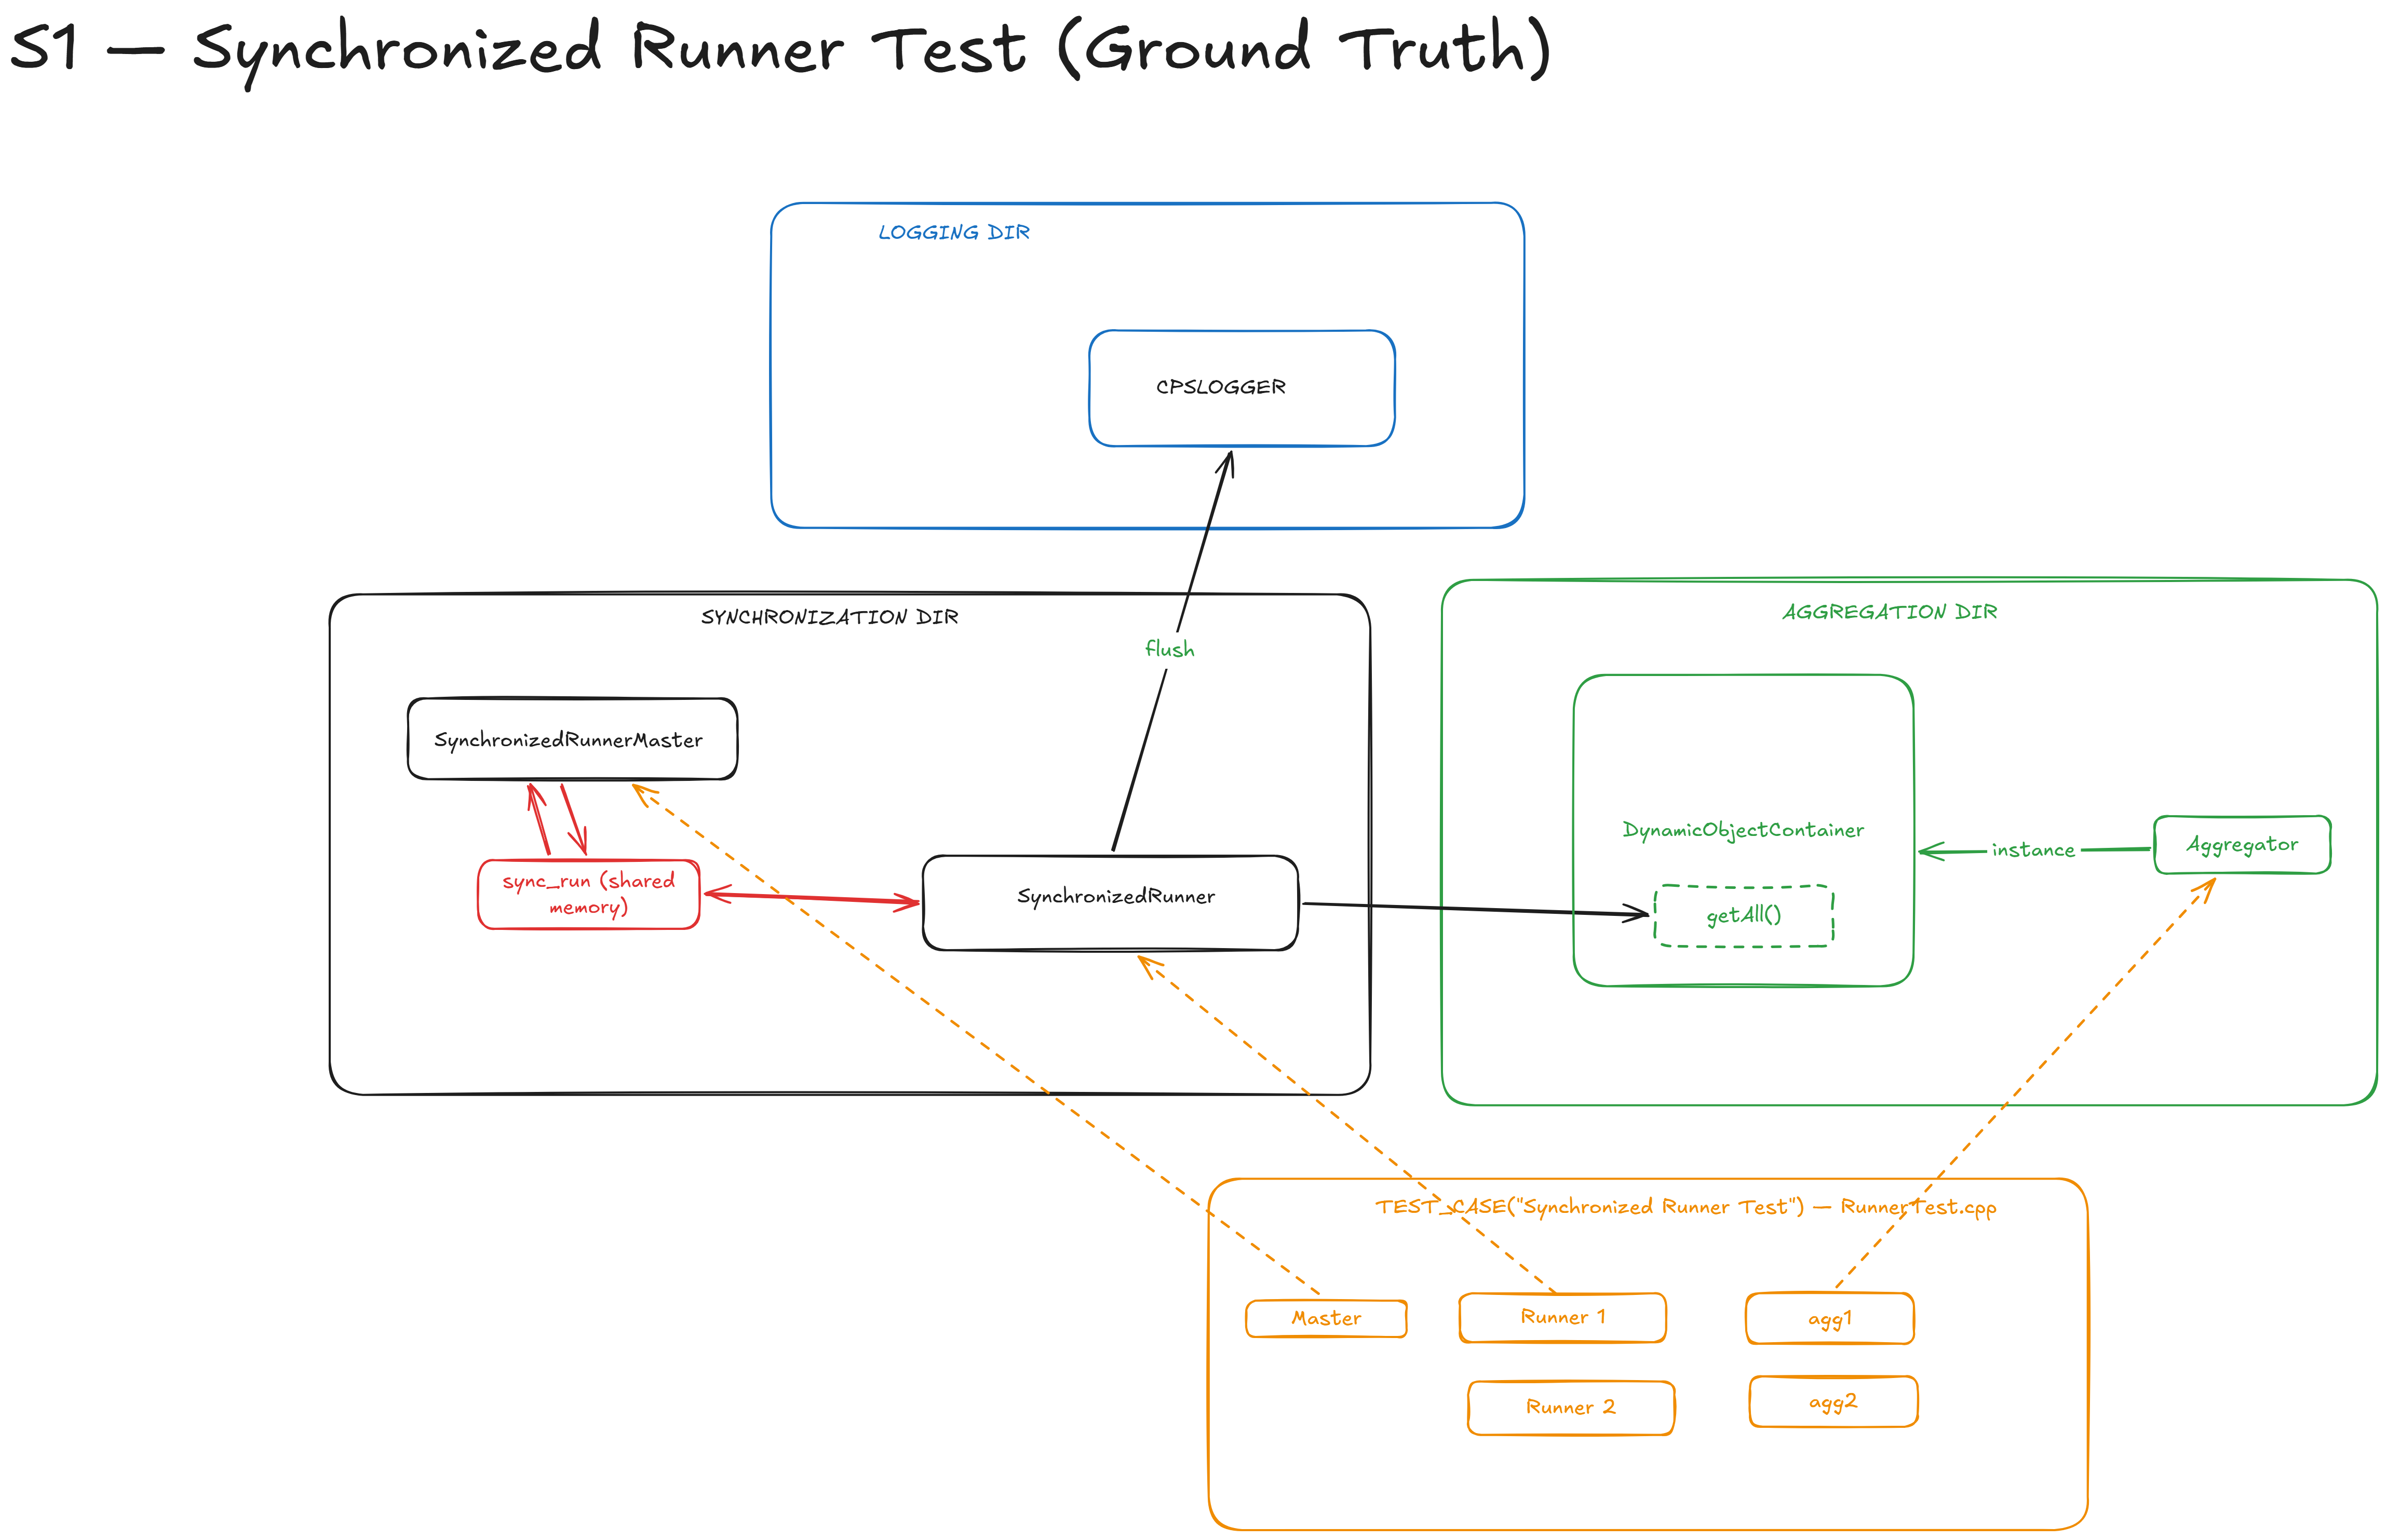
\includegraphics[width=\textwidth]{figures/s1-ground-truth.png}
\caption{Source annotation for S1: the Synchronization/Aggregation/Logging
  call chain exercised by \texttt{SynchronizedRunnerTest}'s happy path.}
\label{fig:s1-groundtruth}
\end{figure}

\subsection{S1: Aggregator Notification Chain, Structural}

\begin{minted}[fontsize=\footnotesize]{text}
package 'S1-Structural' {

    part def Synchronization {
        part synchronizedRunner : SynchronizedRunner;
    }

    part def Aggregation {
        part aggregator : Aggregator;
    }

    part def Logging {
        part cpsLogger : CPSLogger;
    }

    interface def IAggregator {
        in  feature request  : 'getAll';
        out feature response : 'ObjectList';
    }

    interface def ICPSLogger {
        in feature flush : 'flush';
    }

    connection : IAggregator
        connect Synchronization::synchronizedRunner to Aggregation::aggregator;
    connection : ICPSLogger
        connect Synchronization::synchronizedRunner to Logging::cpsLogger;
}
\end{minted}

\subsection{S1: Aggregator Notification Chain, Sequence}

\begin{minted}[fontsize=\footnotesize]{text}
package 'S1-Sequence' {

    part sync : Synchronization;
    part agg  : Aggregation;
    part log  : Logging;

    // SynchronizedRunnerTest: 2x getAll followed by 6x flush
    message m1 from sync.synchronizedRunner to agg.aggregator
        : 'Aggregator.getAll';
    message m2 from sync.synchronizedRunner to agg.aggregator
        : 'Aggregator.getAll';
    message m3 from sync.synchronizedRunner to log.cpsLogger
        : 'CPSLogger.flush';
    message m4 from sync.synchronizedRunner to log.cpsLogger
        : 'CPSLogger.flush';
    message m5 from sync.synchronizedRunner to log.cpsLogger
        : 'CPSLogger.flush';
    message m6 from sync.synchronizedRunner to log.cpsLogger
        : 'CPSLogger.flush';
    message m7 from sync.synchronizedRunner to log.cpsLogger
        : 'CPSLogger.flush';
    message m8 from sync.synchronizedRunner to log.cpsLogger
        : 'CPSLogger.flush';
}
\end{minted}

\begin{figure}[htb]
\centering
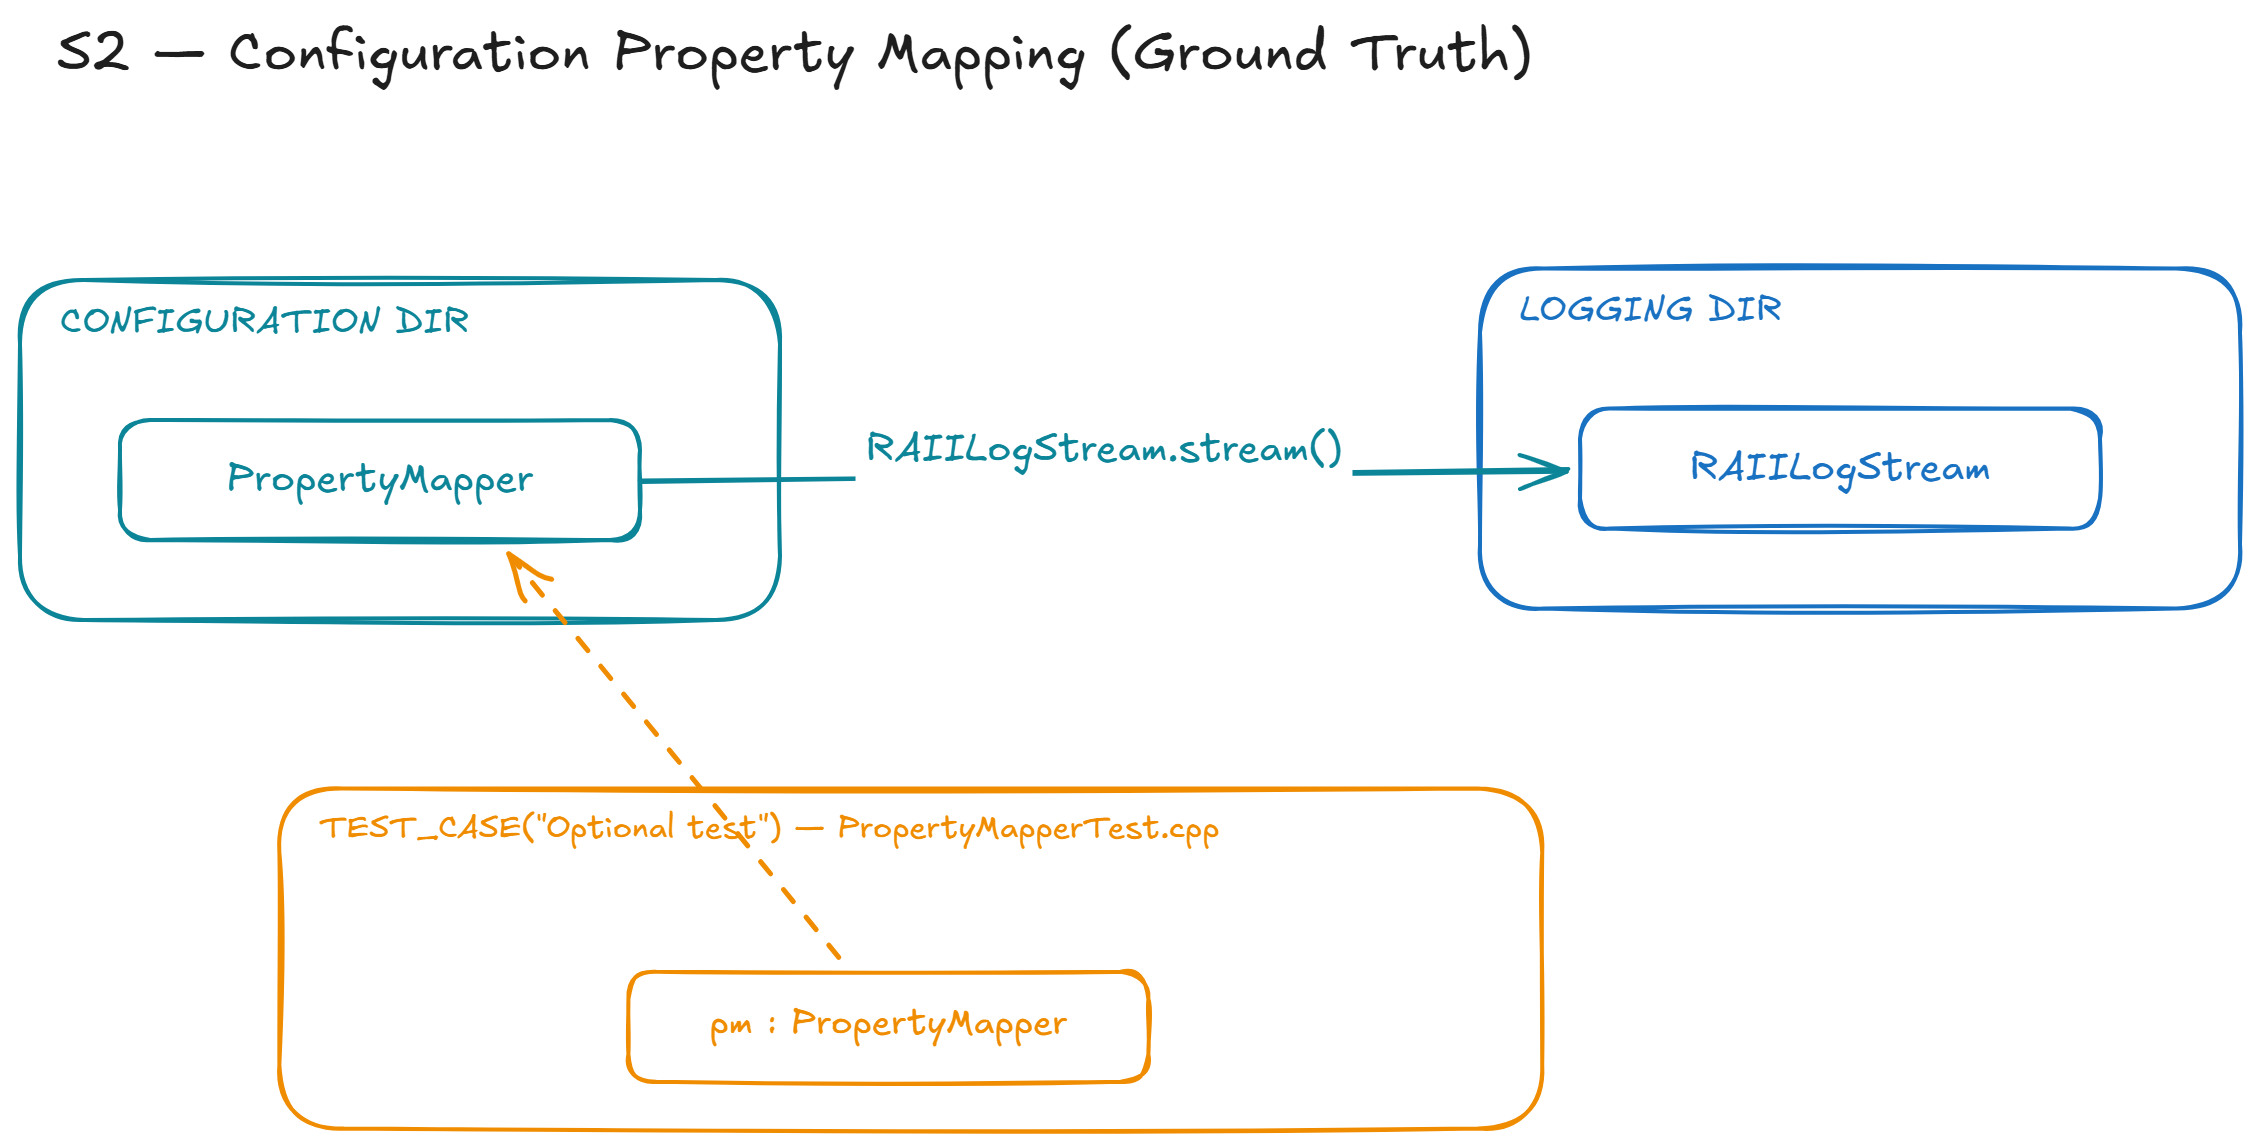
\includegraphics[width=\textwidth]{figures/s2-ground-truth.png}
\caption{S2 ground truth, drawn from direct source inspection: the
  Configuration-to-Logging linear property-mapping chain.}
\label{fig:s2-groundtruth}
\end{figure}

\subsection{S2: Configuration Property Mapping, Structural}

\begin{minted}[fontsize=\footnotesize]{text}
package 'S2-Structural' {

    part def Configuration {
        part propertyMapper : PropertyMapper;
    }

    part def Logging {
        part raiiLogStream : RAIILogStream;
    }

    interface def IRAIILogStream {
        in feature stream : 'stream';
    }

    connection : IRAIILogStream
        connect Configuration::propertyMapper to Logging::raiiLogStream;
}
\end{minted}

\subsection{S2: Configuration Property Mapping, Sequence}

\begin{minted}[fontsize=\footnotesize]{text}
package 'S2-Sequence' {

    part cfg : Configuration;
    part log : Logging;

    message m1 from cfg.propertyMapper to log.raiiLogStream
        : 'RAIILogStream.stream';   // PropertyMapper.add
    message m2 from cfg.propertyMapper to log.raiiLogStream
        : 'RAIILogStream.stream';   // PropertyMapper.add (overload)
    message m3 from cfg.propertyMapper to log.raiiLogStream
        : 'RAIILogStream.stream';   // PropertyMapper.addEigen
    message m4 from cfg.propertyMapper to log.raiiLogStream
        : 'RAIILogStream.stream';   // PropertyMapper.addEnum
    message m5 from cfg.propertyMapper to log.raiiLogStream
        : 'RAIILogStream.stream';   // PropertyMapper.addVector
    message m6 from cfg.propertyMapper to log.raiiLogStream
        : 'RAIILogStream.stream';   // PropertyMapper.getChild
    message m7 from cfg.propertyMapper to log.raiiLogStream
        : 'RAIILogStream.stream';   // PropertyMapper.mandatoryCheck
}
\end{minted}

\begin{figure}[htb]
\centering
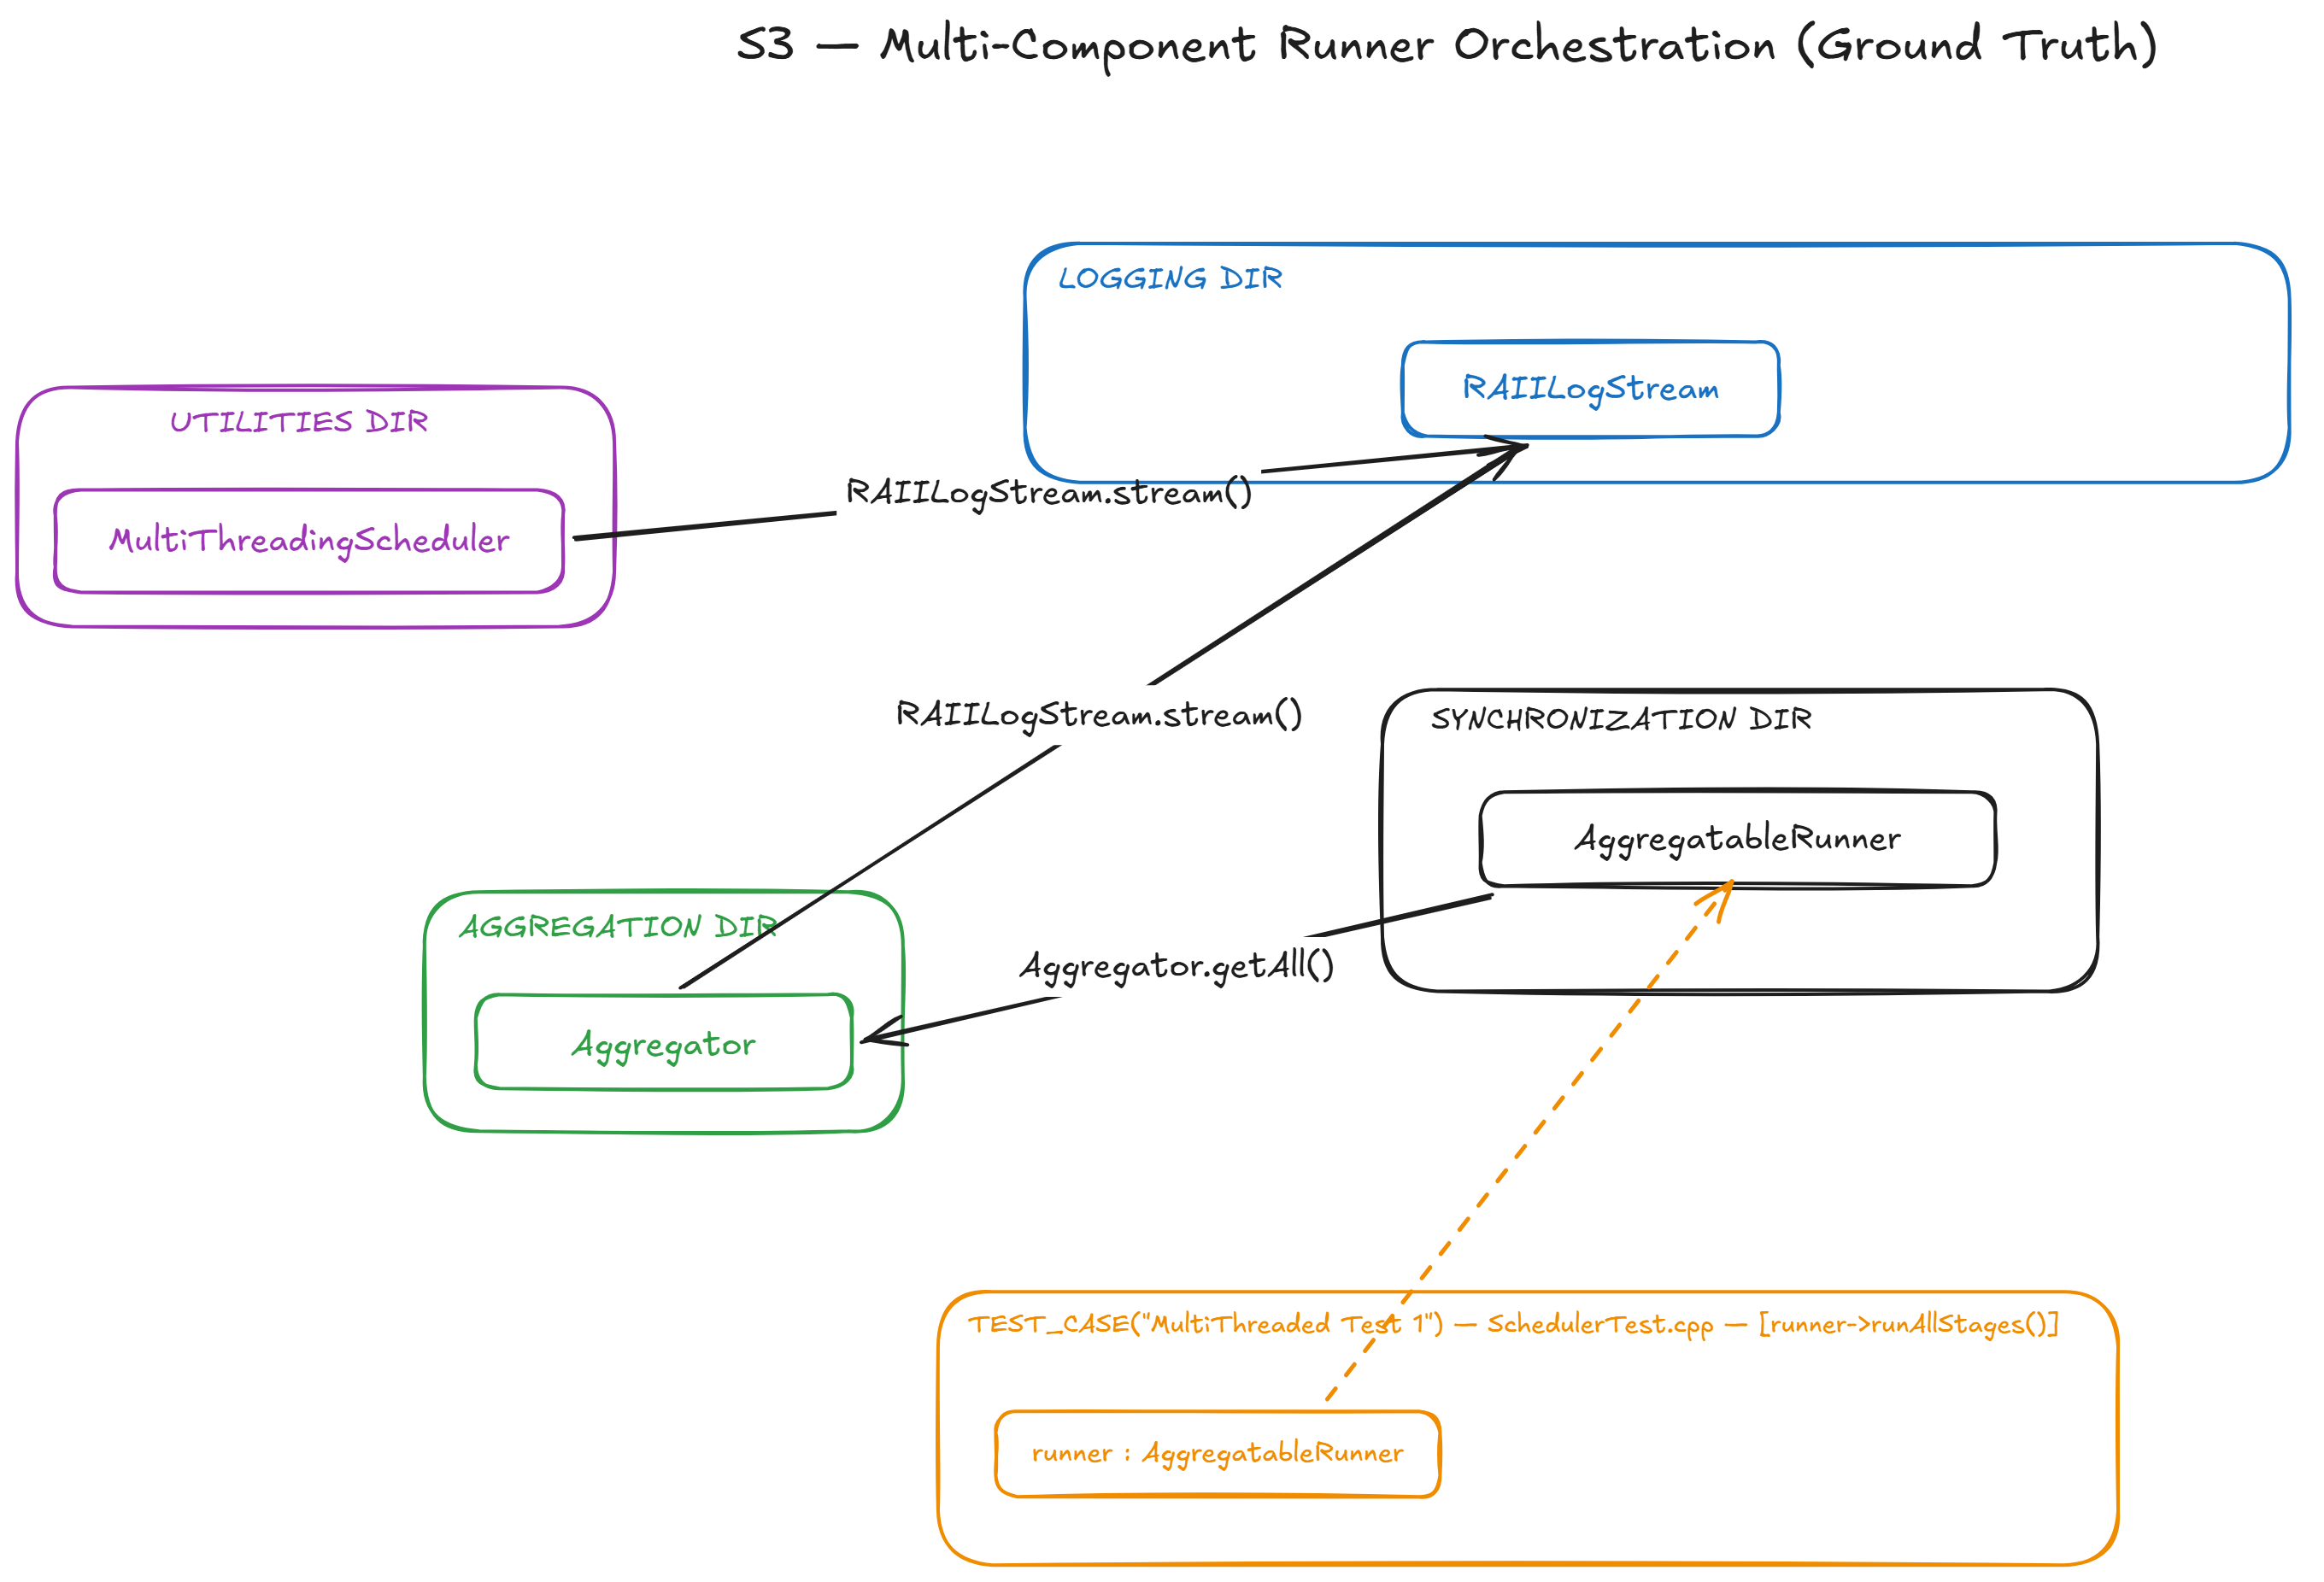
\includegraphics[width=\textwidth]{figures/s3-ground-truth.png}
\caption{S3 ground truth, drawn from direct source inspection: the
  multi-component fan-out from \texttt{AggregatableRunner} into
  Aggregation, Utilities and Logging (\cref{sec:scenarios}).}
\label{fig:s3-groundtruth}
\end{figure}

\subsection{S3: Multi-Component Runner Orchestration, Structural}

\begin{minted}[fontsize=\footnotesize]{text}
package 'S3-Structural' {

    part def Synchronization {
        part aggregatableRunner : AggregatableRunner;
    }

    part def Aggregation {
        part aggregator : Aggregator;
    }

    part def Utilities {
        part scheduler : MultiThreadingScheduler;
    }

    part def Logging {
        part raiiLogStream : RAIILogStream;
    }

    interface def IAggregator {
        in  feature request  : 'getAll';
        out feature response : 'ObjectList';
    }

    interface def IRAIILogStream {
        in feature stream : 'stream';
    }

    connection : IAggregator
        connect Synchronization::aggregatableRunner to Aggregation::aggregator;
    connection : IRAIILogStream
        connect Aggregation::aggregator to Logging::raiiLogStream;
    // Utilities::scheduler dispatches via a std::function-wrapped thread
    // with no resolvable static call site -- invisible to C2, recovered
    // only by the runtime trace (C3), the S3 shortfall discussed in
    // sec:h1-c4c2.
    connection : IRAIILogStream
        connect Utilities::scheduler to Logging::raiiLogStream;
}
\end{minted}

\subsection{S3: Multi-Component Runner Orchestration, Sequence}

\begin{minted}[fontsize=\footnotesize]{text}
package 'S3-Sequence' {

    part sync : Synchronization;
    part agg  : Aggregation;
    part util : Utilities;
    part log  : Logging;

    message m1 from agg.aggregator to log.raiiLogStream
        : 'RAIILogStream.stream';
    message m2 from sync.aggregatableRunner to agg.aggregator
        : 'Aggregator.getAll';
    message m3 from agg.aggregator to log.raiiLogStream
        : 'RAIILogStream.stream';
    message m4 from sync.aggregatableRunner to agg.aggregator
        : 'Aggregator.getAll';
    // Utilities::scheduler's worker thread logs 9 further times,
    // dynamic-only-visible (see structural connection above)
    message m5 from util.scheduler to log.raiiLogStream
        : 'RAIILogStream.stream';
    message m6 from util.scheduler to log.raiiLogStream
        : 'RAIILogStream.stream';
    message m7 from util.scheduler to log.raiiLogStream
        : 'RAIILogStream.stream';
    message m8 from util.scheduler to log.raiiLogStream
        : 'RAIILogStream.stream';
    message m9 from util.scheduler to log.raiiLogStream
        : 'RAIILogStream.stream';
    message m10 from util.scheduler to log.raiiLogStream
        : 'RAIILogStream.stream';
    message m11 from util.scheduler to log.raiiLogStream
        : 'RAIILogStream.stream';
    message m12 from util.scheduler to log.raiiLogStream
        : 'RAIILogStream.stream';
    message m13 from util.scheduler to log.raiiLogStream
        : 'RAIILogStream.stream';
}
\end{minted}

\begin{figure}[htb]
\centering
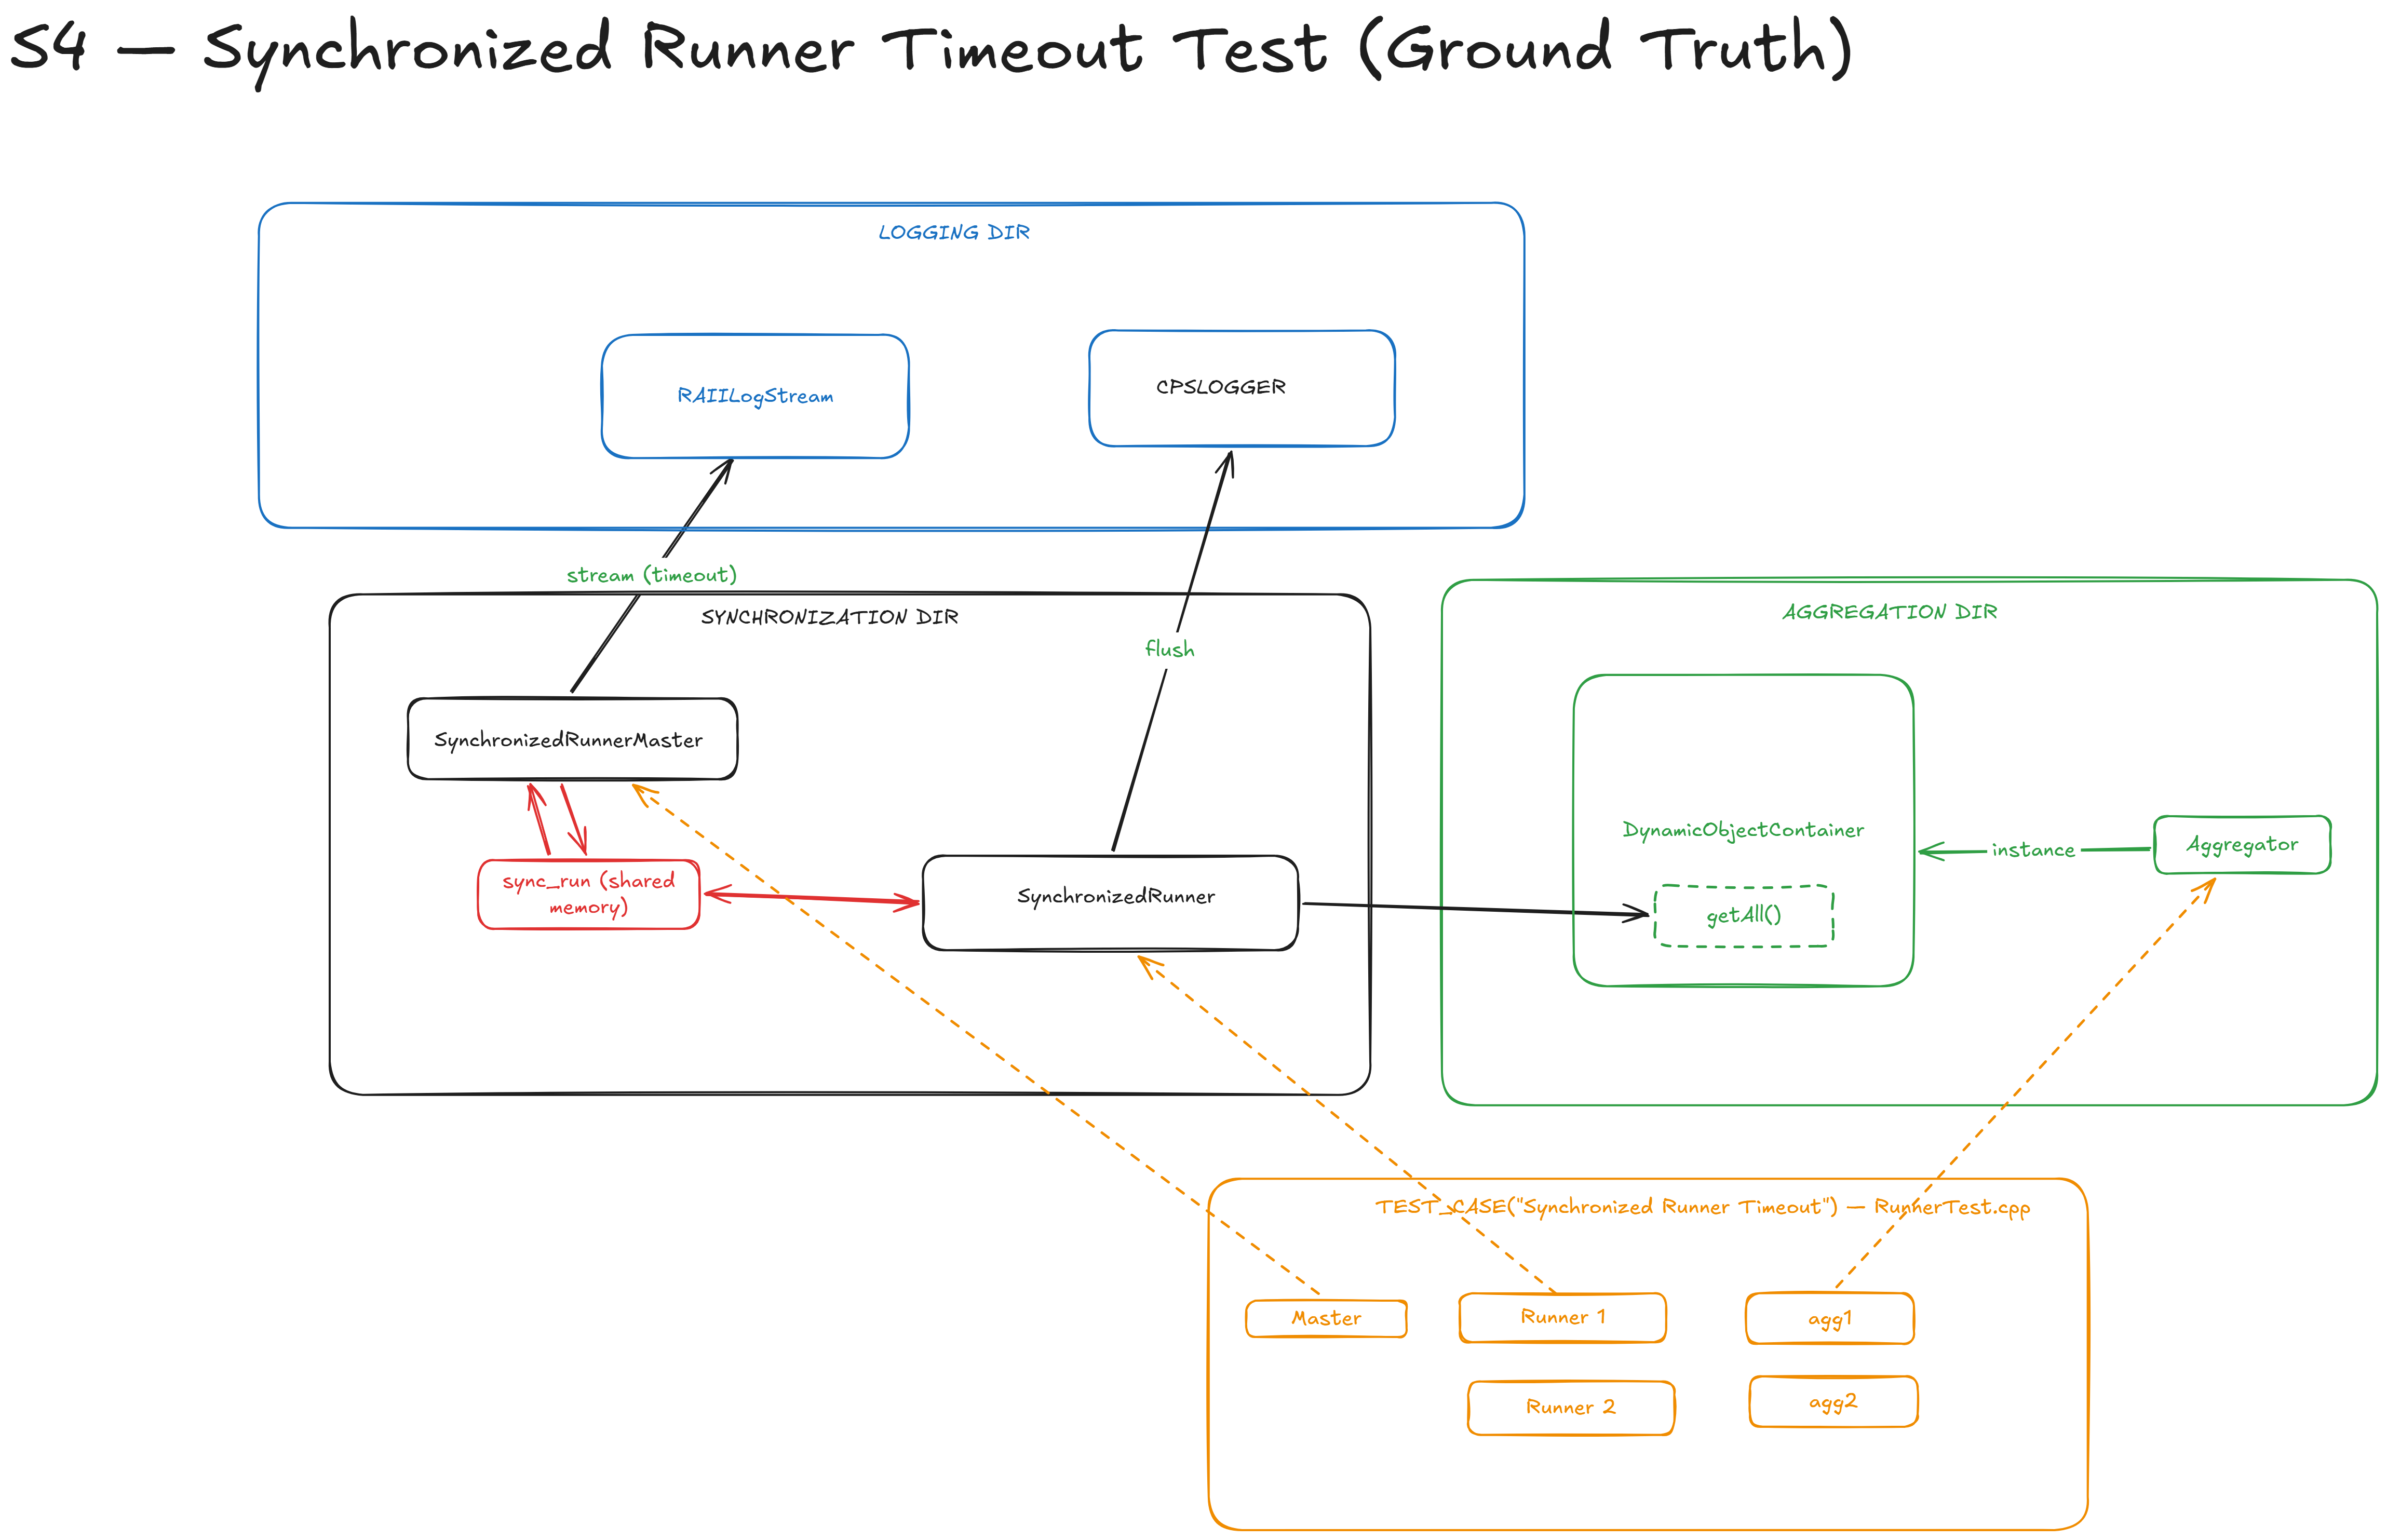
\includegraphics[width=\textwidth]{figures/s1b-ground-truth.png}
\caption{Source annotation for S1b: the same call chain as S1a, exercised
  instead by \texttt{SynchronizedRunnerTest}'s timeout branch, which
  additionally logs via \texttt{RAIILogStream.stream()}.}
\label{fig:s1b-groundtruth}
\end{figure}

\subsection{S1b: Aggregator Notification Chain, Timeout Path, Structural}

\begin{minted}[fontsize=\footnotesize]{text}
package 'S1b-Structural' {

    part def Synchronization {
        part synchronizedRunner : SynchronizedRunner;
    }

    part def Aggregation {
        part aggregator : Aggregator;
    }

    part def Logging {
        part cpsLogger     : CPSLogger;
        part raiiLogStream : RAIILogStream;
    }

    interface def IAggregator {
        in  feature request  : 'getAll';
        out feature response : 'ObjectList';
    }

    interface def ICPSLogger {
        in feature flush : 'flush';
    }

    interface def IRAIILogStream {
        in feature stream : 'stream';
    }

    connection : IAggregator
        connect Synchronization::synchronizedRunner to Aggregation::aggregator;
    connection : ICPSLogger
        connect Synchronization::synchronizedRunner to Logging::cpsLogger;
    connection : IRAIILogStream
        connect Synchronization::synchronizedRunner to Logging::raiiLogStream;
}
\end{minted}

\subsection{S1b: Aggregator Notification Chain, Timeout Path, Sequence}

\begin{minted}[fontsize=\footnotesize]{text}
package 'S1b-Sequence' {

    part sync : Synchronization;
    part agg  : Aggregation;
    part log  : Logging;

    // SynchronizedRunnerTest, timeout branch: 2x getAll, then flush,
    // the timeout log, and one further flush
    message m1 from sync.synchronizedRunner to agg.aggregator
        : 'Aggregator.getAll';
    message m2 from sync.synchronizedRunner to agg.aggregator
        : 'Aggregator.getAll';
    message m3 from sync.synchronizedRunner to log.cpsLogger
        : 'CPSLogger.flush';
    message m4 from sync.synchronizedRunner to log.raiiLogStream
        : 'RAIILogStream.stream';
    message m5 from sync.synchronizedRunner to log.cpsLogger
        : 'CPSLogger.flush';
}
\end{minted}


\section{Generated Pipeline Output}
\label{sec:appendix-generated}

Representative output from the deterministic pipeline (condition~C5,
guided instrumentation + reachability filter,
\cref{sec:h1-results}), shown as component-interaction
edge lists (\texttt{interactions.json}) extracted from the
scenario-scoped edge set.

\subsection{C5 (Guided+Reachability) Edge Lists by Scenario}

\begin{table}[h]
\centering
\caption{Generated component-interaction edges under condition~C5
  (guided instrumentation + reachability filter, F1~$=$~1.000 on all
  four scenarios, \cref{sec:h1-results}).}
\label{tab:c5-edges}
\begin{tabular}{llll}
\toprule
\textbf{Scenario} & \textbf{Source} & \textbf{Target} & \textbf{Interaction} \\
\midrule
S1a & Synchronization & Aggregation & getAll \\
S1a & Synchronization & Logging     & flush \\
\midrule
S1b & Synchronization & Aggregation & getAll \\
S1b & Synchronization & Logging     & flush \\
S1b & Synchronization & Logging     & stream \\
\midrule
S2 & Configuration   & Logging     & stream \\
\midrule
S3 & Synchronization & Aggregation & getAll \\
S3 & Aggregation     & Logging     & stream \\
S3 & Utilities       & Logging     & stream \\
\bottomrule
\end{tabular}
\end{table}

\subsection{Generated SysML~v2 Sequence Model (Excerpt)}

The pipeline also produces a \sysml sequence model with typed messages.
Below is the \emph{Aggregation} scenario, one of 14 auto-generated
scenarios in the complete 800-line output:

\begin{minted}[fontsize=\footnotesize]{text}
part def AggregationScenario :> InteractionScenario {

    part aggregator : Lifeline;
    part dynamicObjectContainer : Lifeline;
    part logger : Lifeline;
    part aggregatableObject : Lifeline;
    part objectHandleContainer : Lifeline;

    part m1 : SynchronousCall {
        ref from : Lifeline = aggregator;
        ref to   : Lifeline = dynamicObjectContainer;
        attribute :>> label = "1. add";
    }
    part m2 : SynchronousCall {
        ref from : Lifeline = aggregator;
        ref to   : Lifeline = dynamicObjectContainer;
        attribute :>> label = "2. notifyAggregationOnUpdate";
    }
    part m3 : SynchronousCall {
        ref from : Lifeline = aggregator;
        ref to   : Lifeline = dynamicObjectContainer;
        attribute :>> label = "3. clear";
    }
    part m4 : SynchronousCall {
        ref from : Lifeline = aggregator;
        ref to   : Lifeline = dynamicObjectContainer;
        attribute :>> label = "4. empty";
    }
    part m5 : SynchronousCall {
        ref from : Lifeline = aggregator;
        ref to   : Lifeline = dynamicObjectContainer;
        attribute :>> label = "5. size";
    }
    part m6 : SynchronousCall {
        ref from : Lifeline = aggregator;
        ref to   : Lifeline = logger;
        attribute :>> label = "6. stream";
    }
}
\end{minted}

\section{Generated Mermaid Diagrams}
\label{sec:appendix-mermaid}

The pipeline also produces Mermaid diagrams for module-level structural
views. The module-dependency diagram below, generated from the static
call graph in \neo, summarises cross-directory call edges:

\begin{minted}[fontsize=\footnotesize]{text}
flowchart TD
  subgraph SRC["src"]
    direction TB
    Aggregation["Aggregation (function defs: 17)"]
    Configuration["Configuration (function defs: 9)"]
    Framework["Framework (function defs: 9)"]
    Logging["Logging (function defs: 12)"]
    Synchronization["Synchronization (function defs: 14)"]
    Utilities["Utilities (function defs: 174)"]
  end

  Utilities -->|"calls (13)"| Logging
  Synchronization -->|"calls (3)"| Aggregation
  Synchronization -->|"calls (3)"| Logging
  Utilities -->|"calls (2)"| Configuration
  Synchronization -->|"calls (2)"| Utilities
  Aggregation -->|"calls (1)"| Utilities
  Logging -->|"calls (1)"| Utilities
\end{minted}

The runtime-tracing diagram below shows how \texttt{SignalHandler}
interacts with logging, IPC, and scheduler components, with static call
edges (solid) and runtime subscription edges (dashed):

\begin{minted}[fontsize=\footnotesize]{text}
flowchart TD
  subgraph SignalDir["src/Utilities/SignalHandler"]
    sh_exit["subscribeOnExit()"]
    sh_sigint["subscribeOnSigint()"]
    sh_handler["sigIntHandler()"]
  end

  subgraph LoggingAPI["include/cpsCore/Logging"]
    raii_stream["RAIILogStream.stream()"]
  end

  subgraph IPCDir["src/Utilities/IPC"]
    IPC_cpp["IPC.cpp (runtime subscriber)"]
  end

  subgraph SchedulerDir["src/Utilities/Scheduler"]
    Sched_cpp["MultiThreadingScheduler.cpp (runtime subscriber)"]
  end

  sh_exit --> raii_stream
  sh_sigint --> raii_stream
  IPC_cpp -.->|signal subscription| SignalDir
  Sched_cpp -.->|signal subscription| SignalDir
\end{minted}

\section{Rendered Diagram Figures}
\label{sec:appendix-rendered}

Rendered versions of the diagrams from the preceding sections. Source
\texttt{.mmd} files and both PNG and SVG outputs are in the
\texttt{figures/} directory of the repository.

\begin{figure}[htbp]
  \centering
  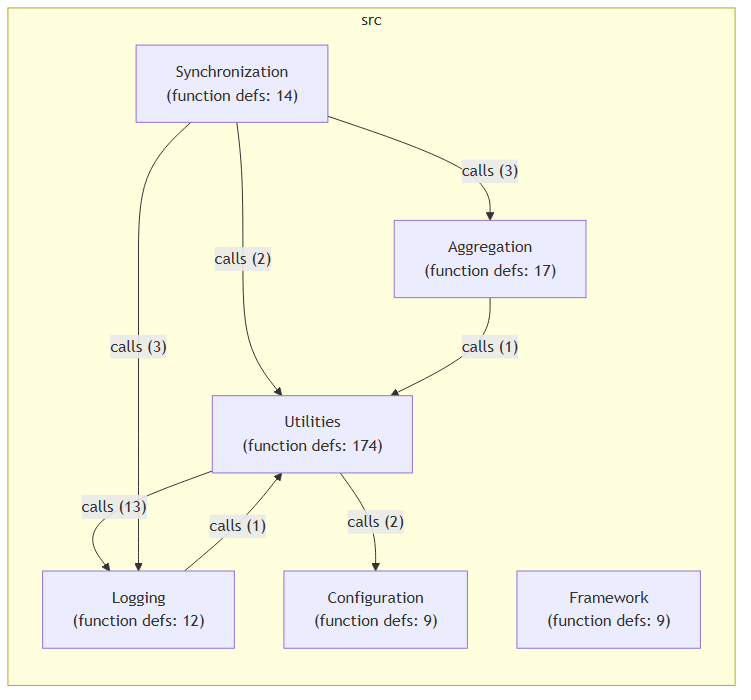
\includegraphics[width=0.85\textwidth]{figures/module-dependency.png}
  \caption{Module-level dependency structure of CPSCore (cross-directory call edges).}
  \label{fig:module-dep}
\end{figure}

\begin{figure}[htbp]
  \centering
  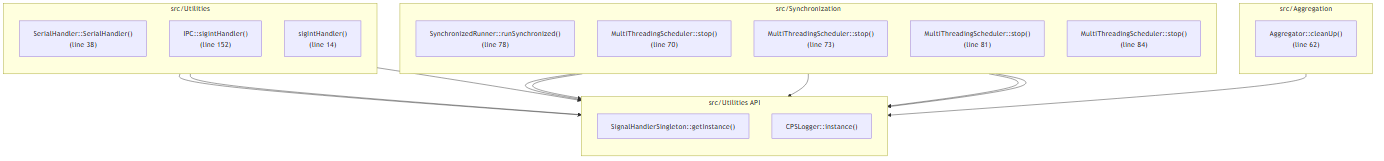
\includegraphics[width=0.9\textwidth]{figures/function-call-dependencies.png}
  \caption{Cross-module function-call dependencies to singleton APIs.}
  \label{fig:func-deps}
\end{figure}

\begin{figure}[htbp]
  \centering
  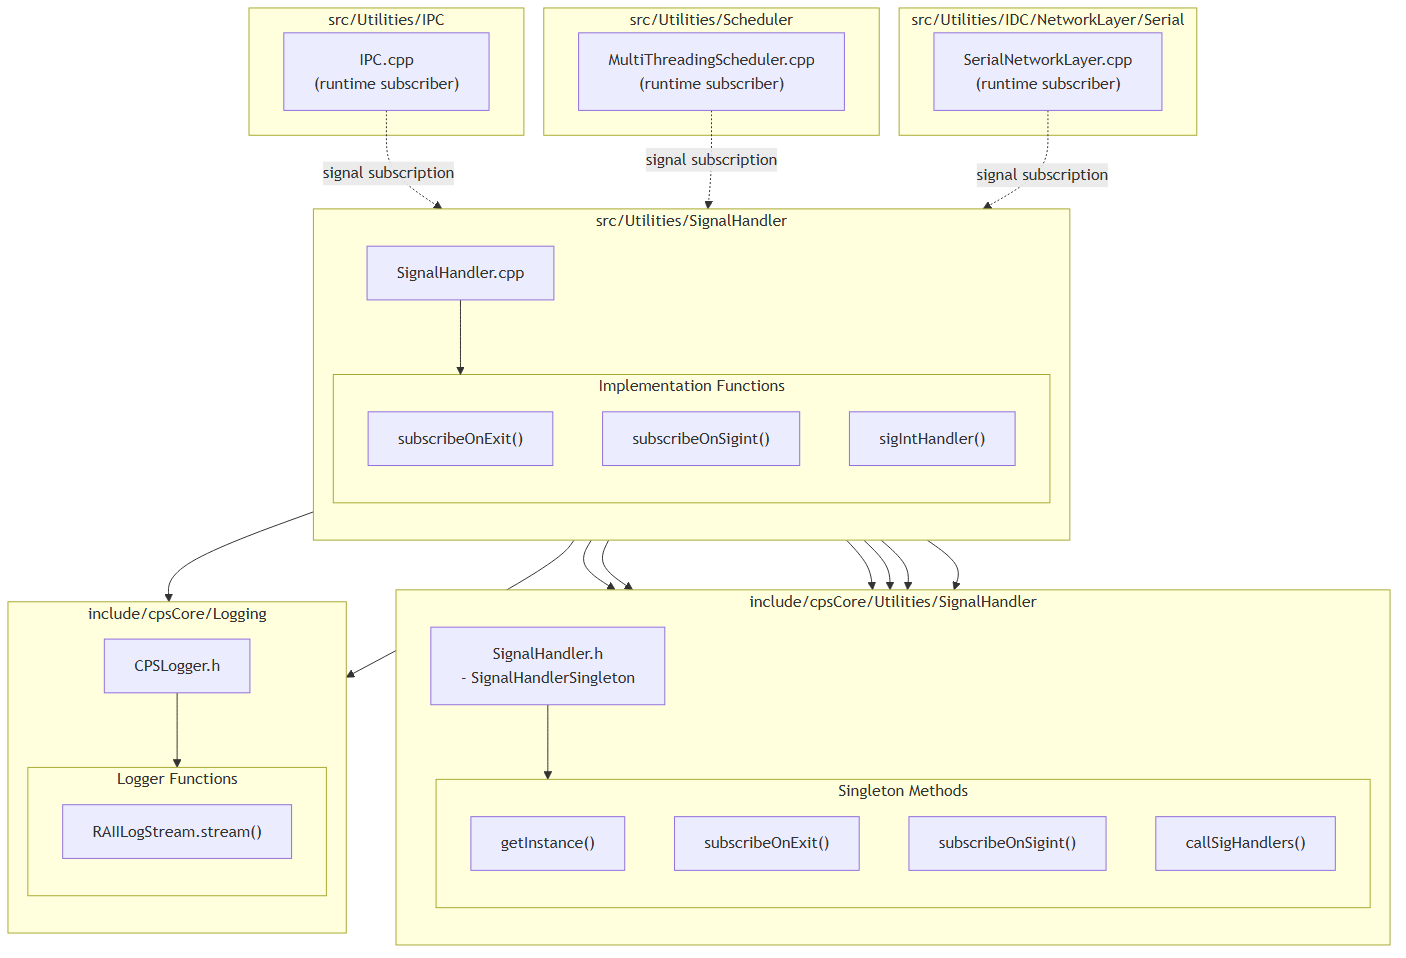
\includegraphics[width=0.85\textwidth]{figures/signal-runtime-tracing.png}
  \caption{SignalHandler subsystem: static call edges (solid) and runtime subscriptions (dashed).}
  \label{fig:signal-tracing}
\end{figure}

\subsection{Rendered Diagrams: S1a, S1b, S2, S3 (Illustrative)}
\label{sec:appendix-c5-rendered}

The figures below are rendered artefacts for all four scenarios: the
interconnection diagram (the assembled system with real port-to-port
\texttt{connect} statements, the same artefact discussed in
\cref{sec:sysml-generation}) and the sequence diagram
(\texttt{draw-sysml-sequence-model}). They are rendered from condition~C5
(guided instrumentation + reachability filter,
\cref{sec:evidence-synthesis}) and therefore match the edge lists in
\cref{tab:c5-edges} exactly. Compare against the ground-truth
diagrams in \cref{sec:appendix-groundtruth}.

\begin{figure}[htbp]
  \centering
  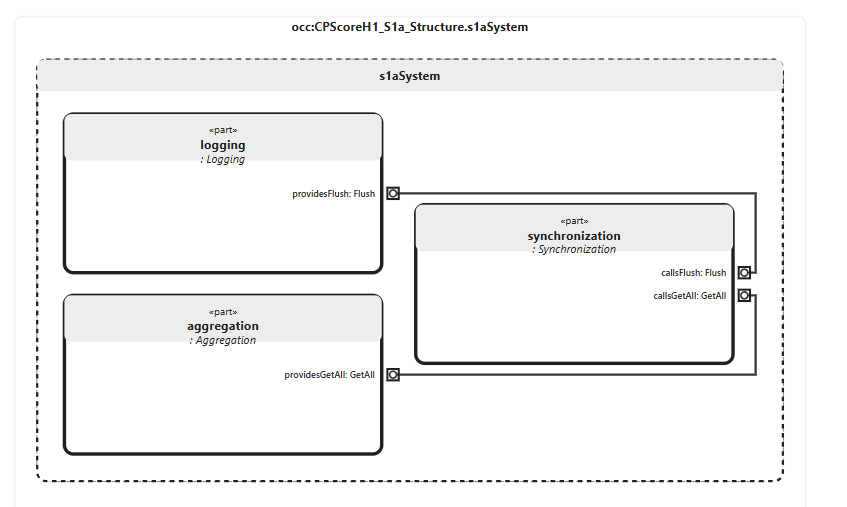
\includegraphics[width=0.75\textwidth]{figures/s1a-interconnection.png}
  \caption{S1 (Aggregator notification chain): interconnection diagram.}
  \label{fig:s1-interconnection}
\end{figure}

\begin{figure}[htbp]
  \centering
  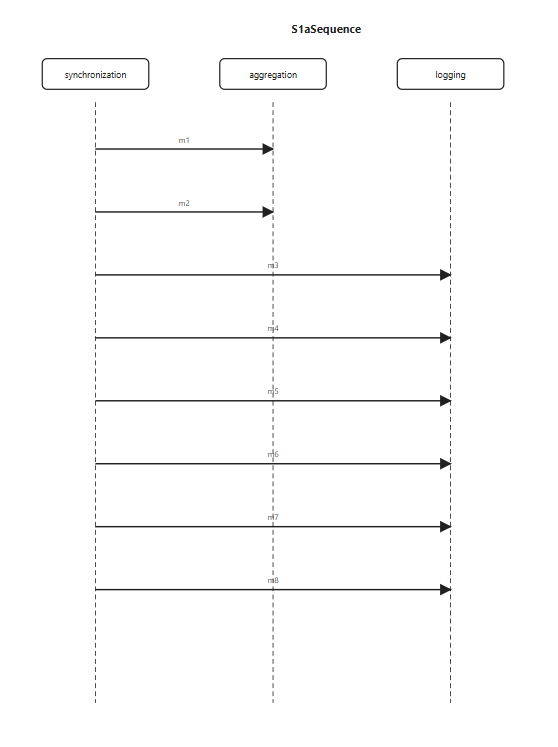
\includegraphics[width=0.6\textwidth]{figures/s1a-sequence.png}
  \caption{S1 sequence diagram: message interactions.}
  \label{fig:s1-seq}
\end{figure}

\begin{figure}[htbp]
  \centering
  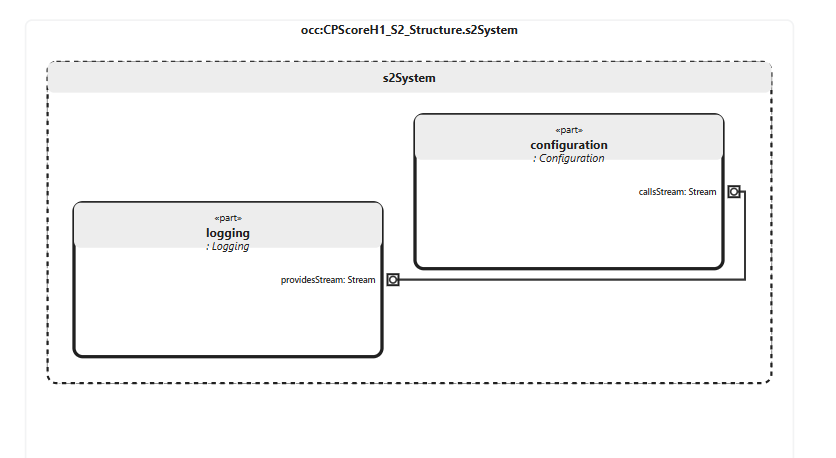
\includegraphics[width=0.75\textwidth]{figures/s2-interconnection.png}
  \caption{S2 (Configuration property mapping): interconnection diagram.}
  \label{fig:s2-interconnection}
\end{figure}

\begin{figure}[htbp]
  \centering
  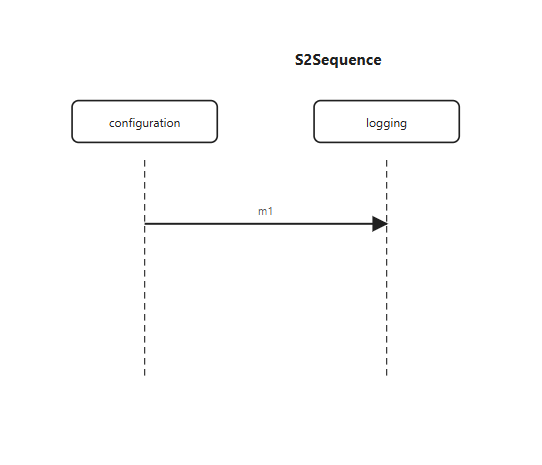
\includegraphics[width=0.6\textwidth]{figures/s2-sequence.png}
  \caption{S2 sequence diagram: Configuration property mapping.}
  \label{fig:s2-seq}
\end{figure}

\begin{figure}[htbp]
  \centering
  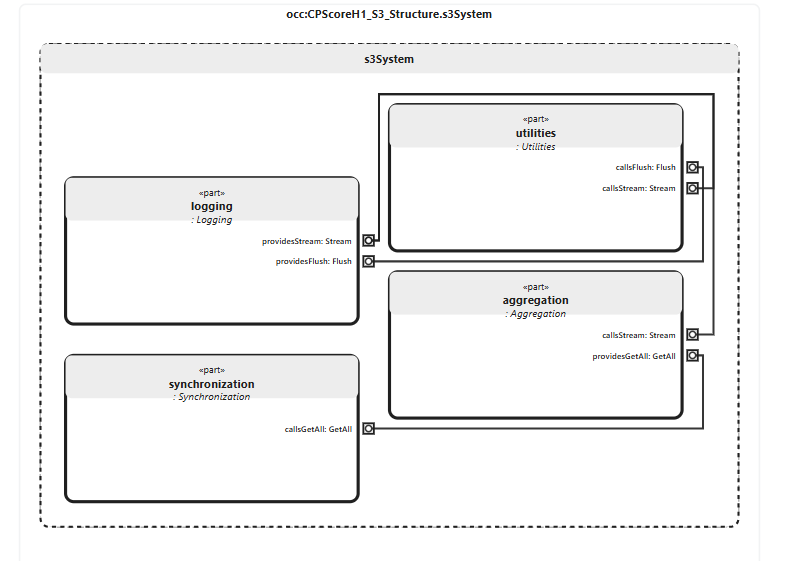
\includegraphics[width=0.75\textwidth]{figures/s3-interconnection.png}
  \caption{S3 (multi-component runner orchestration): interconnection diagram.}
  \label{fig:s3-interconnection}
\end{figure}

\begin{figure}[htbp]
  \centering
  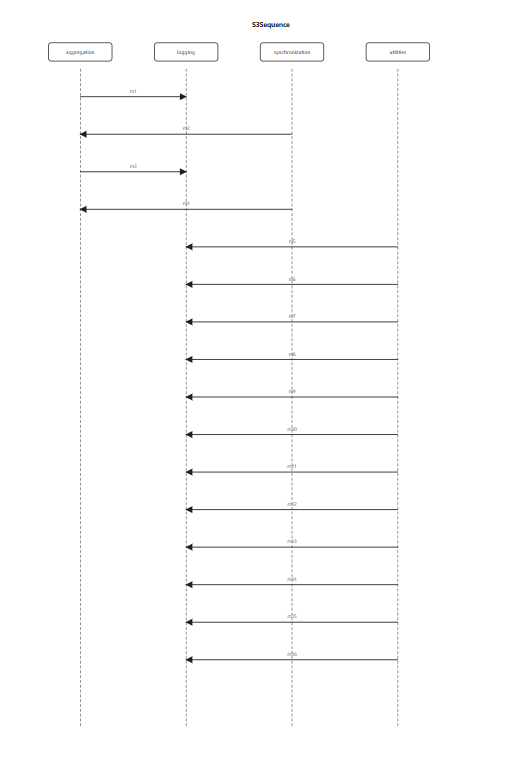
\includegraphics[width=0.6\textwidth]{figures/s3-sequence.png}
  \caption{S3 sequence diagram: multi-component runner orchestration.}
  \label{fig:s3-seq}
\end{figure}

\begin{figure}[htbp]
  \centering
  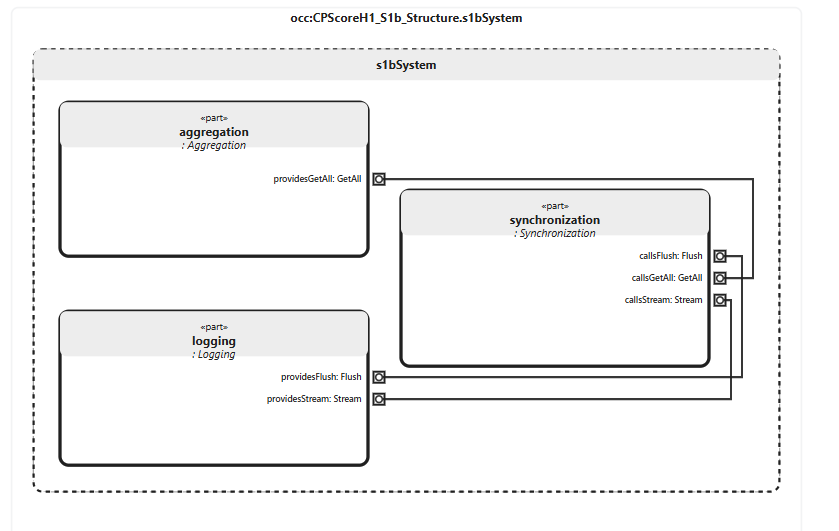
\includegraphics[width=0.75\textwidth]{figures/s1b-interconnection.png}
  \caption{S1b (Aggregator notification chain, timeout path): interconnection diagram.}
  \label{fig:s1b-interconnection}
\end{figure}

\begin{figure}[htbp]
  \centering
  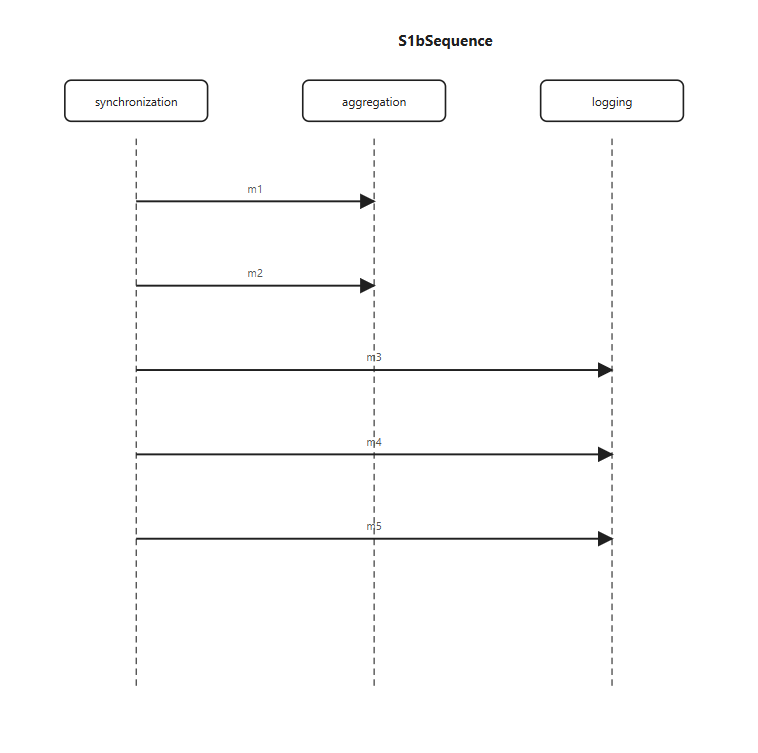
\includegraphics[width=0.6\textwidth]{figures/s1b-sequence.png}
  \caption{S1b sequence diagram: Aggregator notification chain, timeout path.}
  \label{fig:s1b-seq}
\end{figure}

\section{H2 Qualitative Arm: Per-Rater Decomposition}
\label{sec:appendix-h2-perrater}

This appendix records the per-rater decomposition and free-text analysis
behind the blinded expert rating study summarised in
\cref{sec:h2-qual}. The aggregate results (\cref{tab:h2-qual-results})
are given in the main text; the detail below supports the claim that
the accuracy/readability effect is unanimous in direction, and that the
only genuine split is usefulness on S2.

One rater, R4, consistently rated the two conditions closer together
than the other five: R4 accounts for two of the six accuracy ties (S2,
S3), one of the six usefulness ties (S1), and the dataset's only
reversal, rating full instrumentation's usefulness above guided's on S2
(4 vs.\ 3). No rater ever rated full instrumentation higher on
accuracy or readability on any scenario, so that effect is unanimous in
direction (never reversed, though twice tied); usefulness is unanimous
on S1 and S3 but genuinely mixed on S2.

The free-text comments explain why. On S1 and S3, five of six raters
independently described the guided diagram as retaining only the
components named in the scenario context and starting at the correct
point in the sequence, while calling the full-instrumentation diagram
more complete but cluttered with additional \texttt{stream} events not
obviously relevant without prior codebase knowledge. One rater (R1),
while still preferring the guided diagram overall, flagged a residual
\texttt{instance} call retained in guided S1 as ``also superfluous'',
a reminder that H2's noise$=0$ result (\cref{sec:h2-results}) is scoped
to the reference set used for scoring, not to what a domain expert reading
the diagram cold considers extraneous; the two need not coincide.

S2 shows the same pattern in reverse: the guided diagram collapses seven
repeated \texttt{Configuration}$\to$\texttt{Logging} property-read calls
into a single edge, and five of six raters
rated it more accurate and more readable for matching the two components
named in the scenario. Usefulness is where the panel genuinely splits.
Three raters (R1--R3) tied it, each independently citing the same
reason: collapsing the reads loses a \emph{count} they considered
relevant to debugging, even though it played no part in their accuracy
or readability judgement. R4 rated full instrumentation \emph{more}
useful on S2, for a distinct reason: with the guided diagram alone ``it
is not clear what triggers a logging event.'' Only R5 and R6 rated
guided as more useful outright. Usefulness on S2 is therefore a genuine
three-way split (tied, reversed, and in favour of guided) rather than
the clean 2-rater tie originally reported from the smaller panel.

Several raters converged independently on the same suggestions for
handling high-volume \texttt{stream} events: R3 and R6 suggested a
toggle/filter to distinguish them rather than always including or
omitting them; R2 suggested recording the specific property value
emitted by each \texttt{stream} call, so the collapsed S2 edge stays
useful for debugging without losing its readability advantage; and R3
additionally proposed a two-stage workflow: full instrumentation to see
where an interaction sits in the broader flow, then guided
instrumentation to reason about the scenario itself. This reframes full
instrumentation as a complementary, coarser-grained view rather than a
failed alternative.

\section{SysML v2 Generated Diagrams}
\label{sec:appendix-sysmlv2}

The following figures show the SysML v2 diagrams generated for the
CPSCore case study: structural (component connectivity) and sequence
(interaction flow) diagrams for the 14 bulk, whole-codebase scenarios
(\cref{sec:sysml-impl}), generated directly from the unscoped static
sequence dependency table rather than from any scenario-scoped H1
condition.

\subsection{Structural Diagrams}

\begin{figure}[htbp]
  \centering
  
\includegraphics[width=\textwidth]{figures/sysmlv2 diagrams/structure.png}
  \caption{Complete CPSCore component model: all part definitions and interface connections.}
  \label{fig:sysml-structure}
\end{figure}

\begin{figure}[htbp]
  \centering
  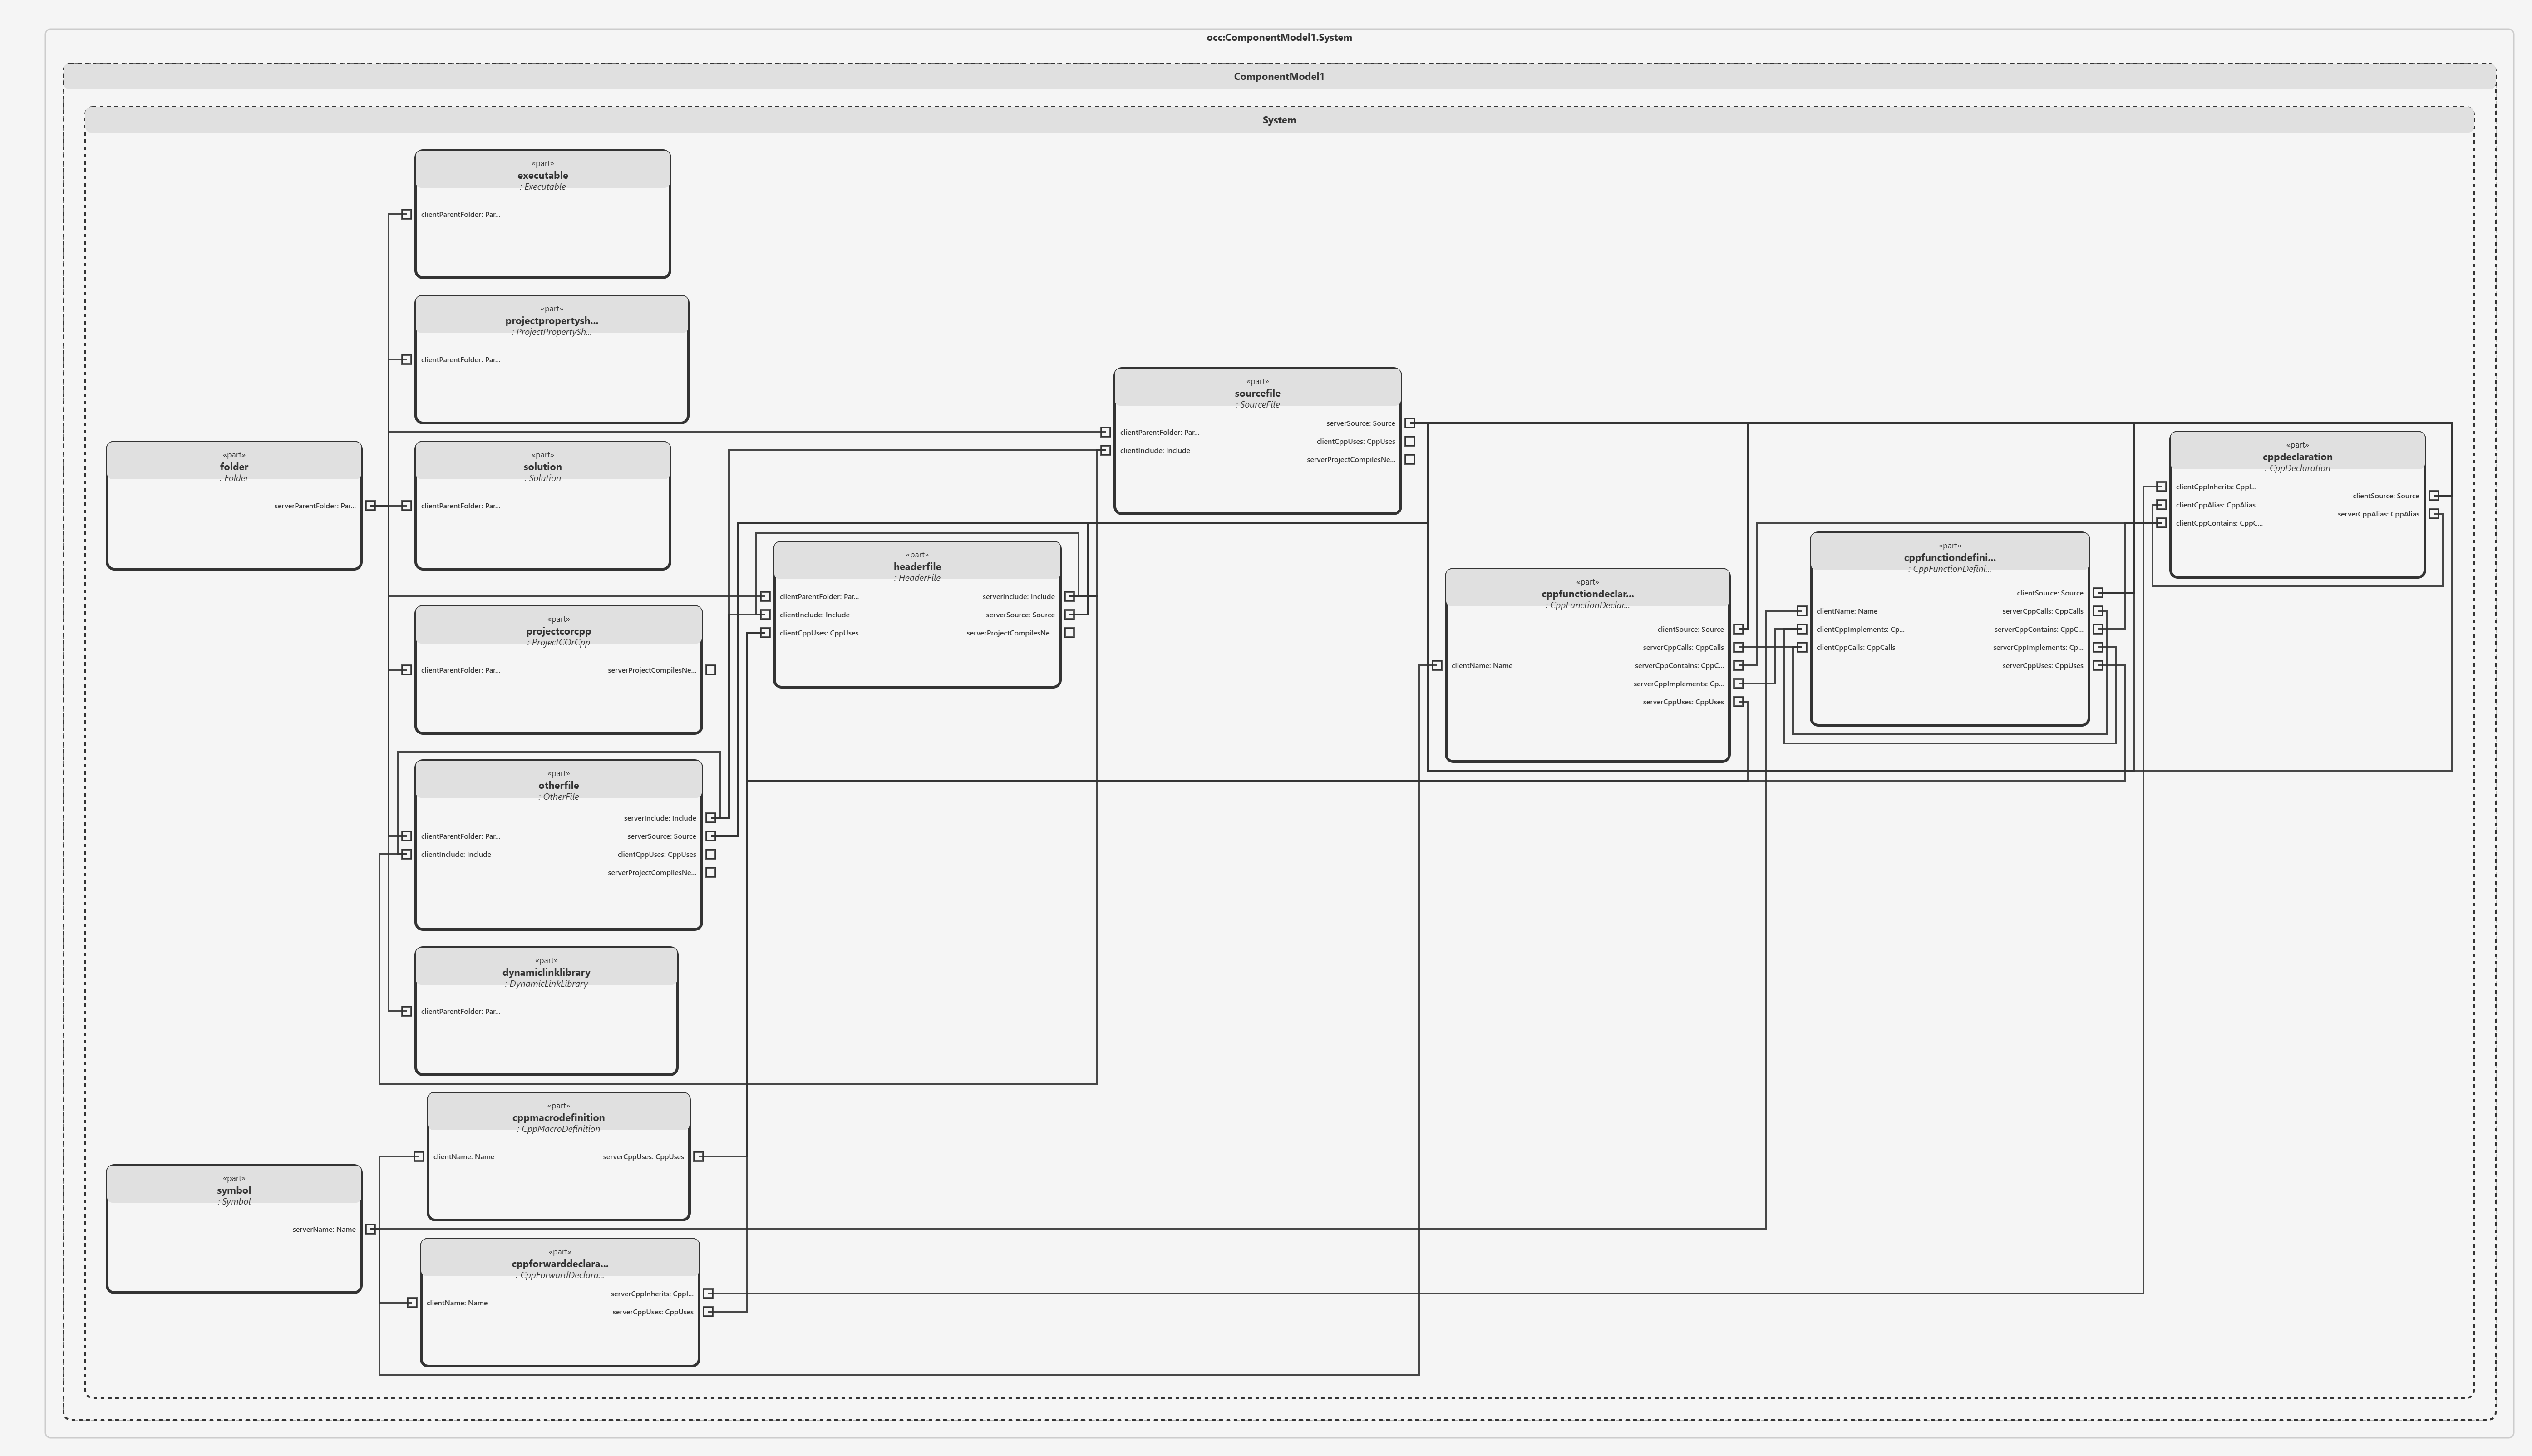
\includegraphics[width=\textwidth]{figures/sysmlv2 diagrams/connections.png}
  \caption{Node-type hierarchy and property graph schema relationships (13 node labels).}
  \label{fig:sysml-connections}
\end{figure}

\subsection{Sequence Diagrams}

\begin{figure}[htbp]
  \centering
  \begin{subfigure}[t]{0.48\textwidth}
    \centering
    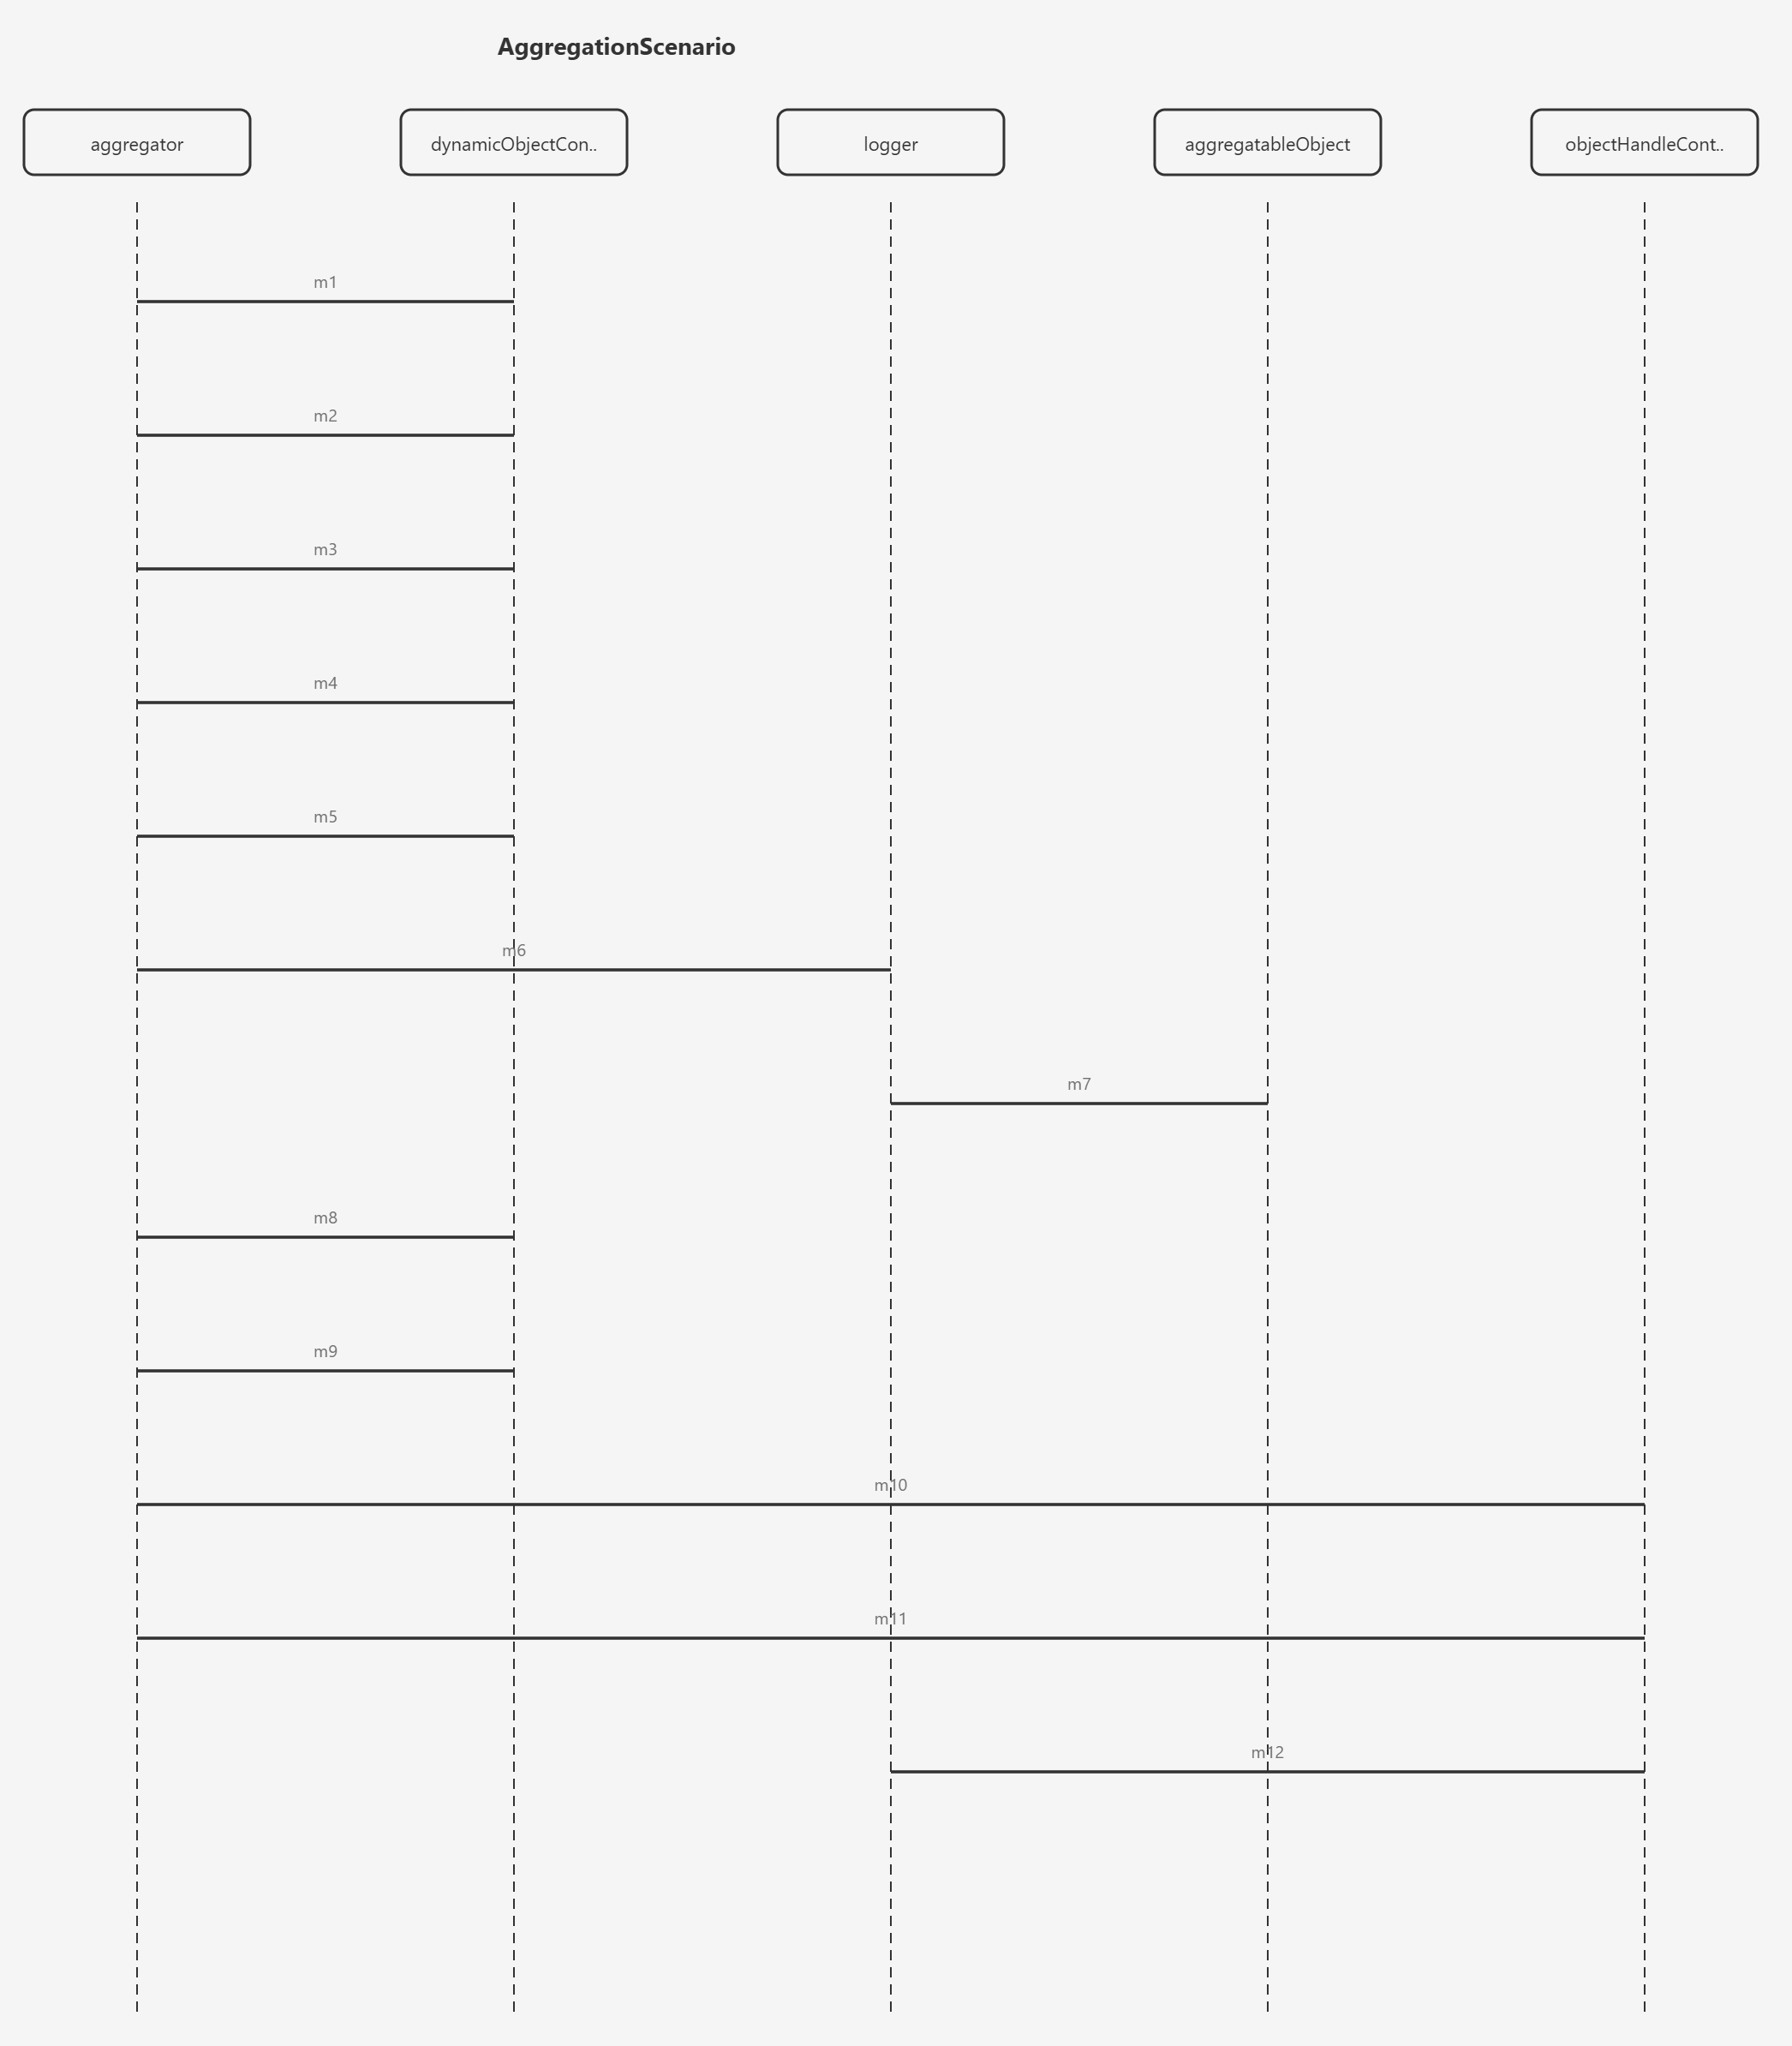
\includegraphics[width=\linewidth]{figures/sysmlv2 diagrams/aggregationFlow.png}
    \caption{Aggregation scenario: component wiring and lifecycle interactions
      (Aggregator, DynamicObjectContainer, Logger, AggregatableObject).}
    \label{fig:sysml-aggregation}
  \end{subfigure}
  \hfill
  \begin{subfigure}[t]{0.48\textwidth}
    \centering
    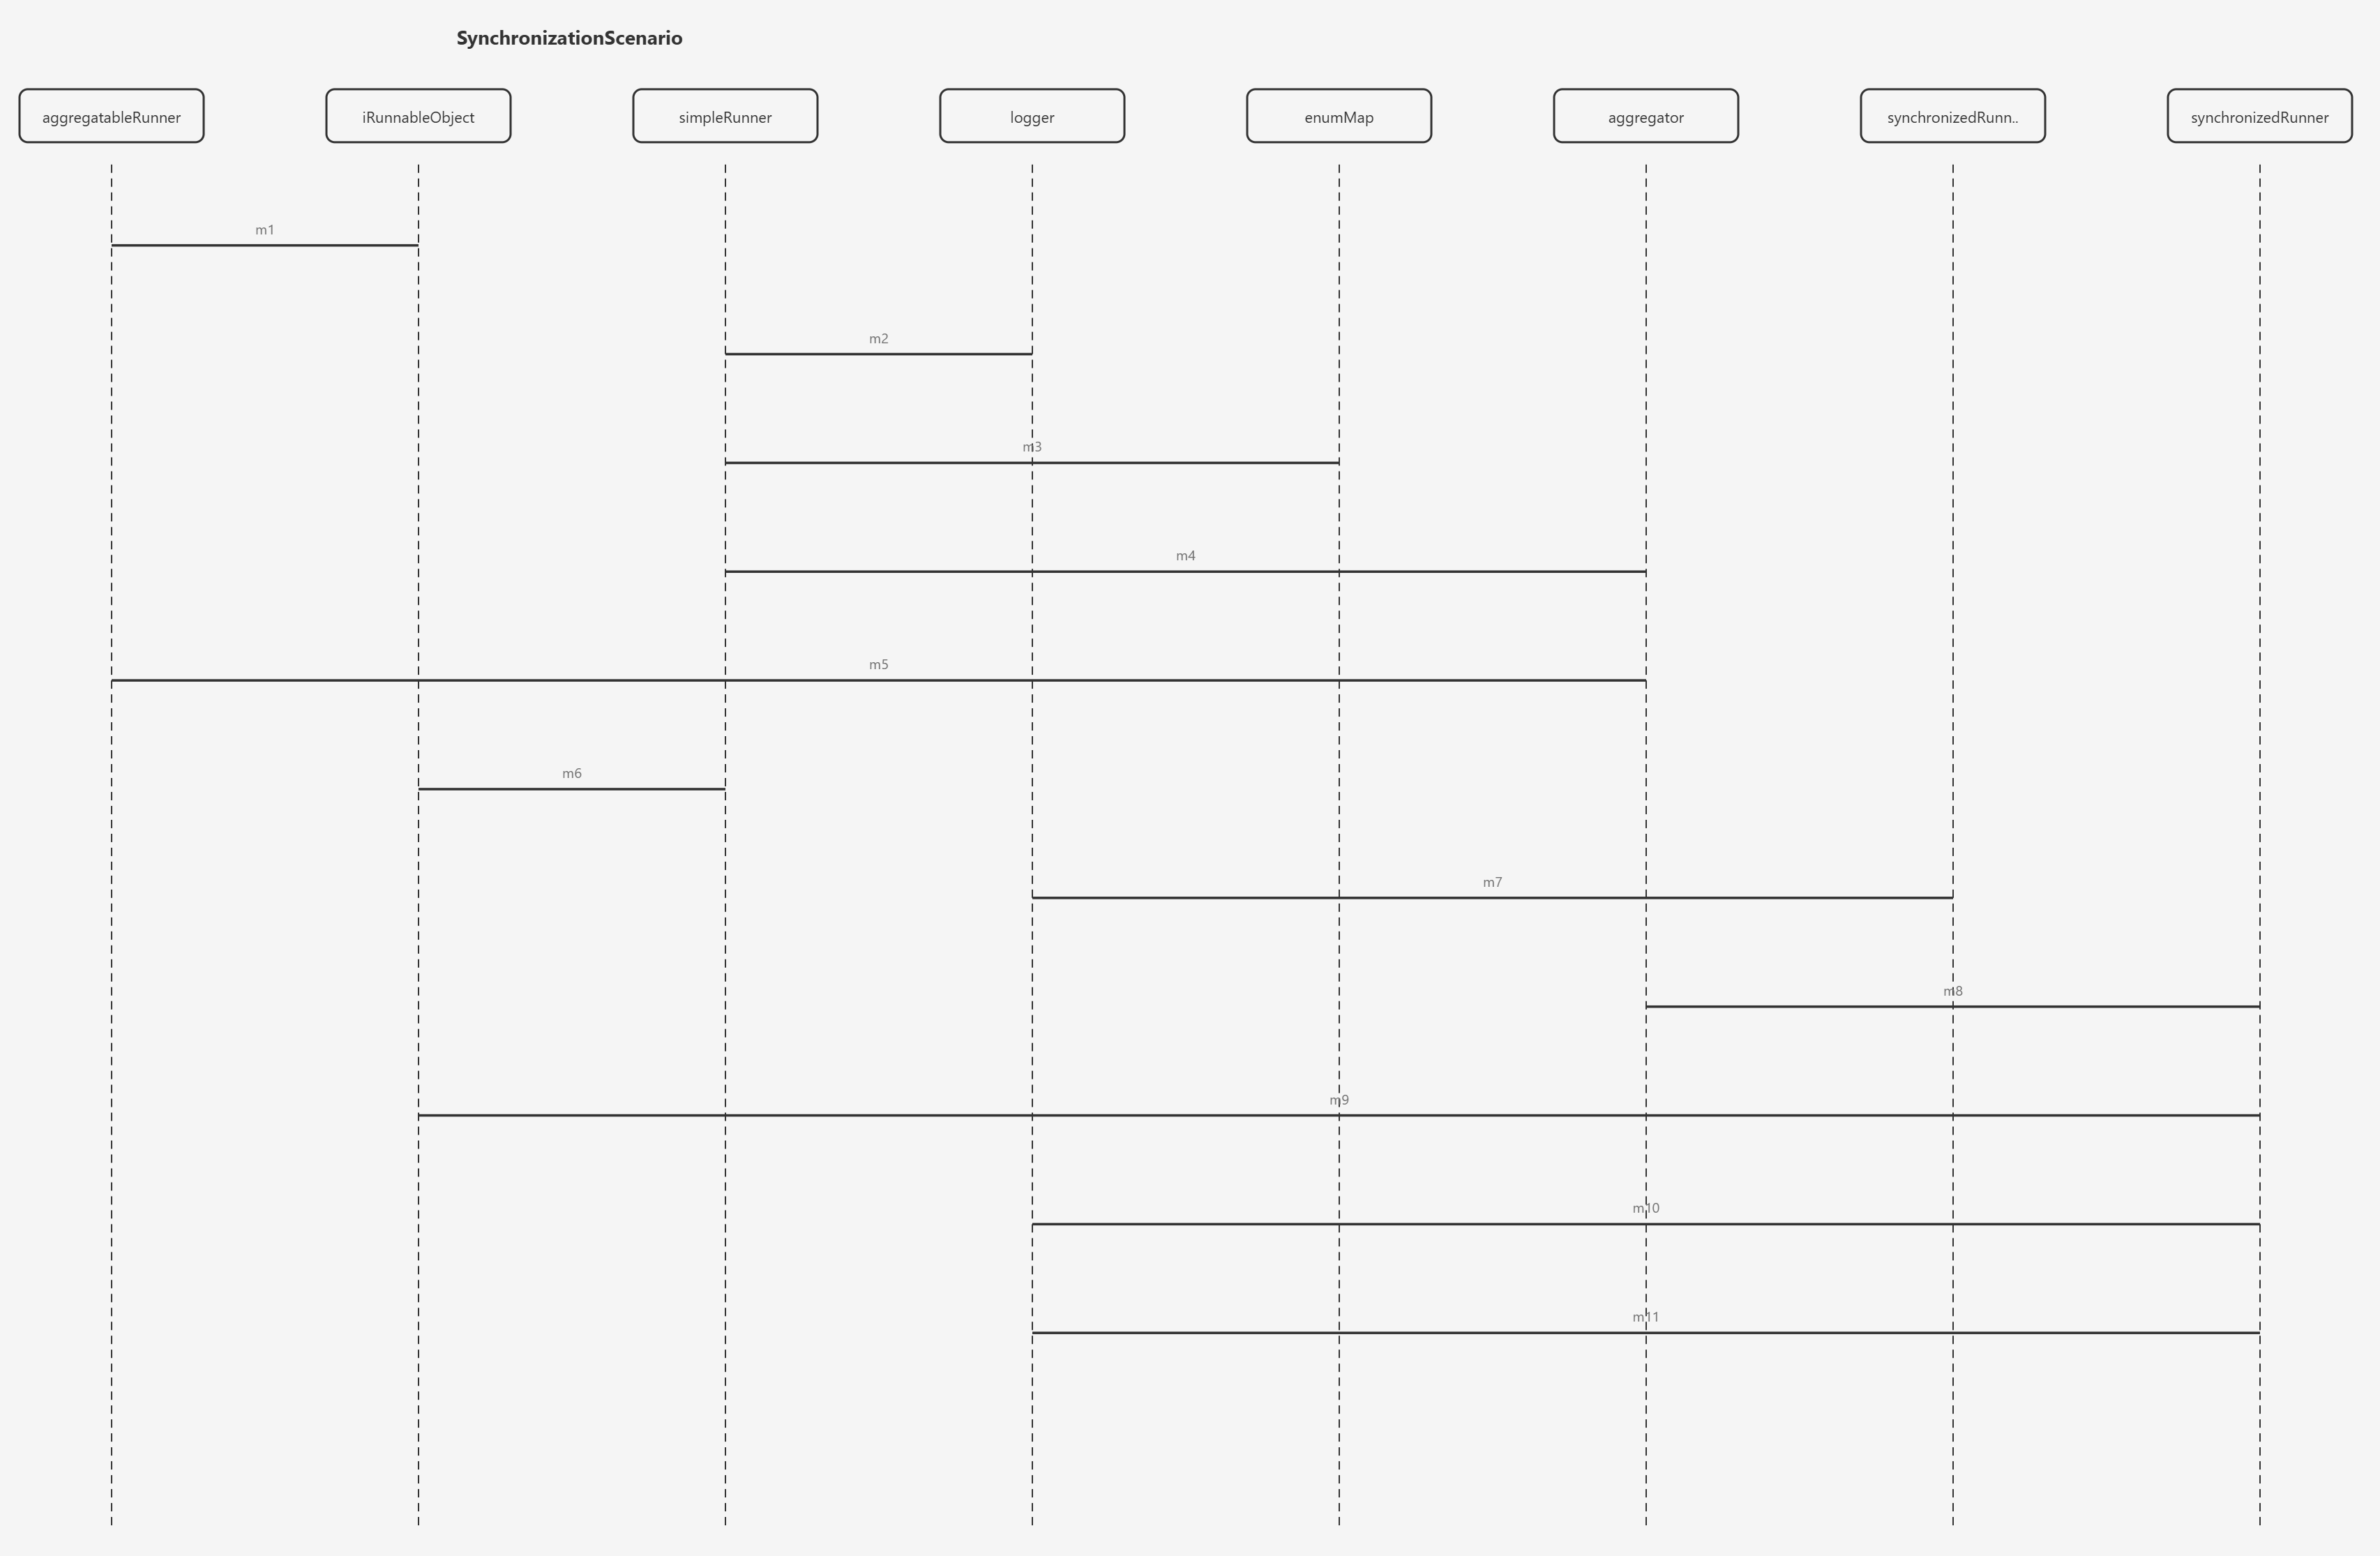
\includegraphics[width=\linewidth]{figures/sysmlv2 diagrams/synchronizationFlow.png}
    \caption{Synchronization scenario: run-stage scheduling interactions
      (AggregatableRunner, IRunnableObject, SimpleRunner, Logger, EnumMap,
      Aggregator, SynchronizedRunnerMaster, SynchronizedRunner).}
    \label{fig:sysml-synchronization}
  \end{subfigure}
  \caption{SysML v2 sequence diagrams: Aggregation (left) and Synchronization (right).}
\end{figure}

\begin{figure}[H]
  \centering
  \begin{subfigure}[t]{0.48\textwidth}
    \centering
    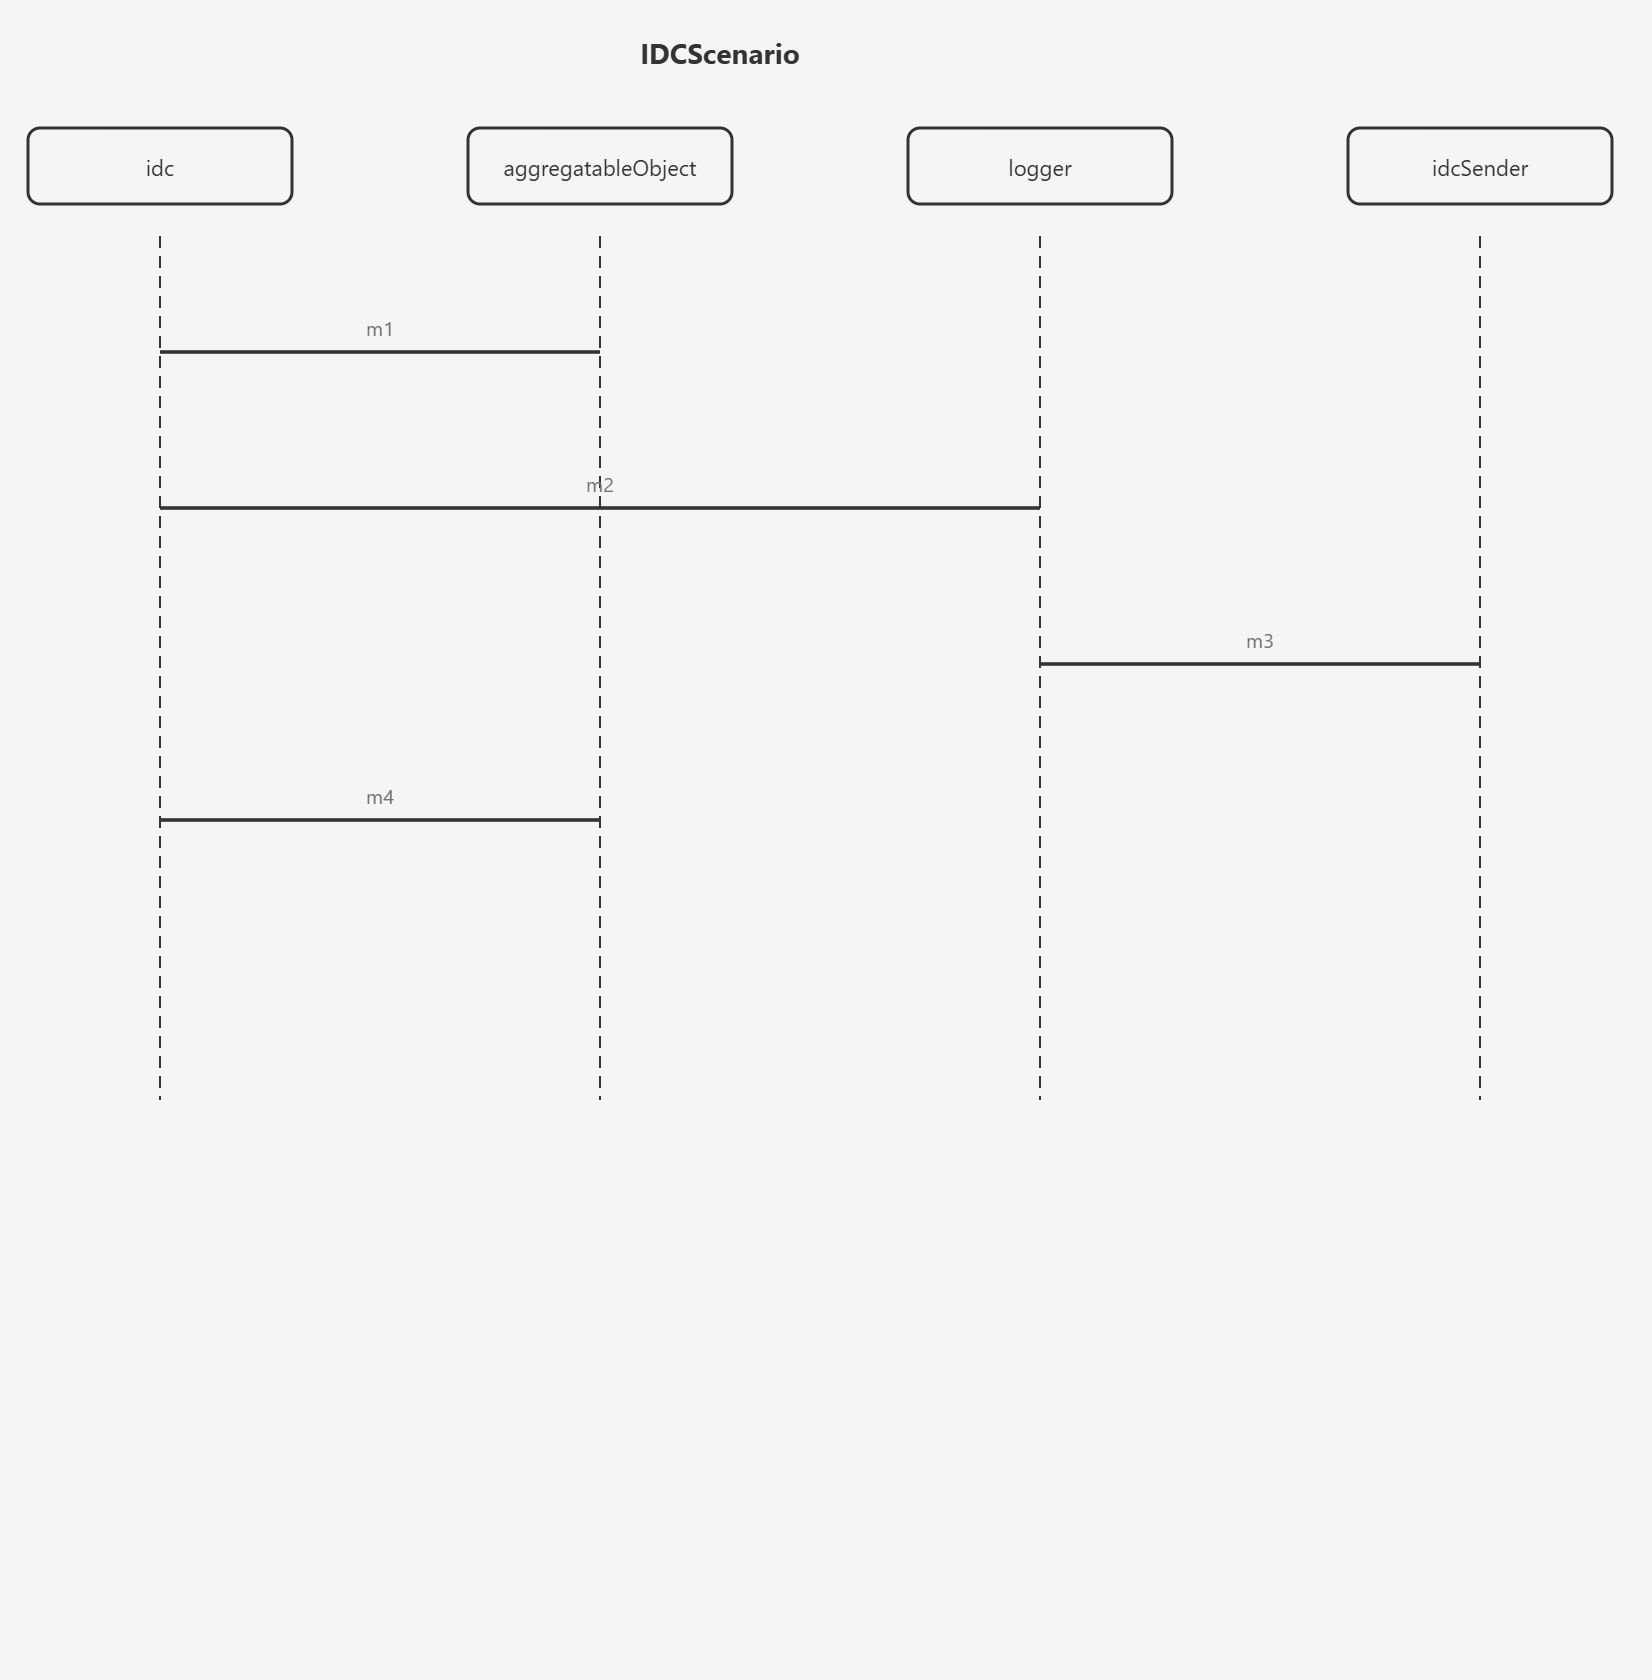
\includegraphics[width=\linewidth]{figures/sysmlv2 diagrams/idcFlow.png}
    \caption{IDC scenario: inter-component communication through the IDC
      abstraction layer (IDC, AggregatableObject, Logger, IDCSender).}
    \label{fig:sysml-idc}
  \end{subfigure}
  \hfill
  \begin{subfigure}[t]{0.48\textwidth}
    \centering
    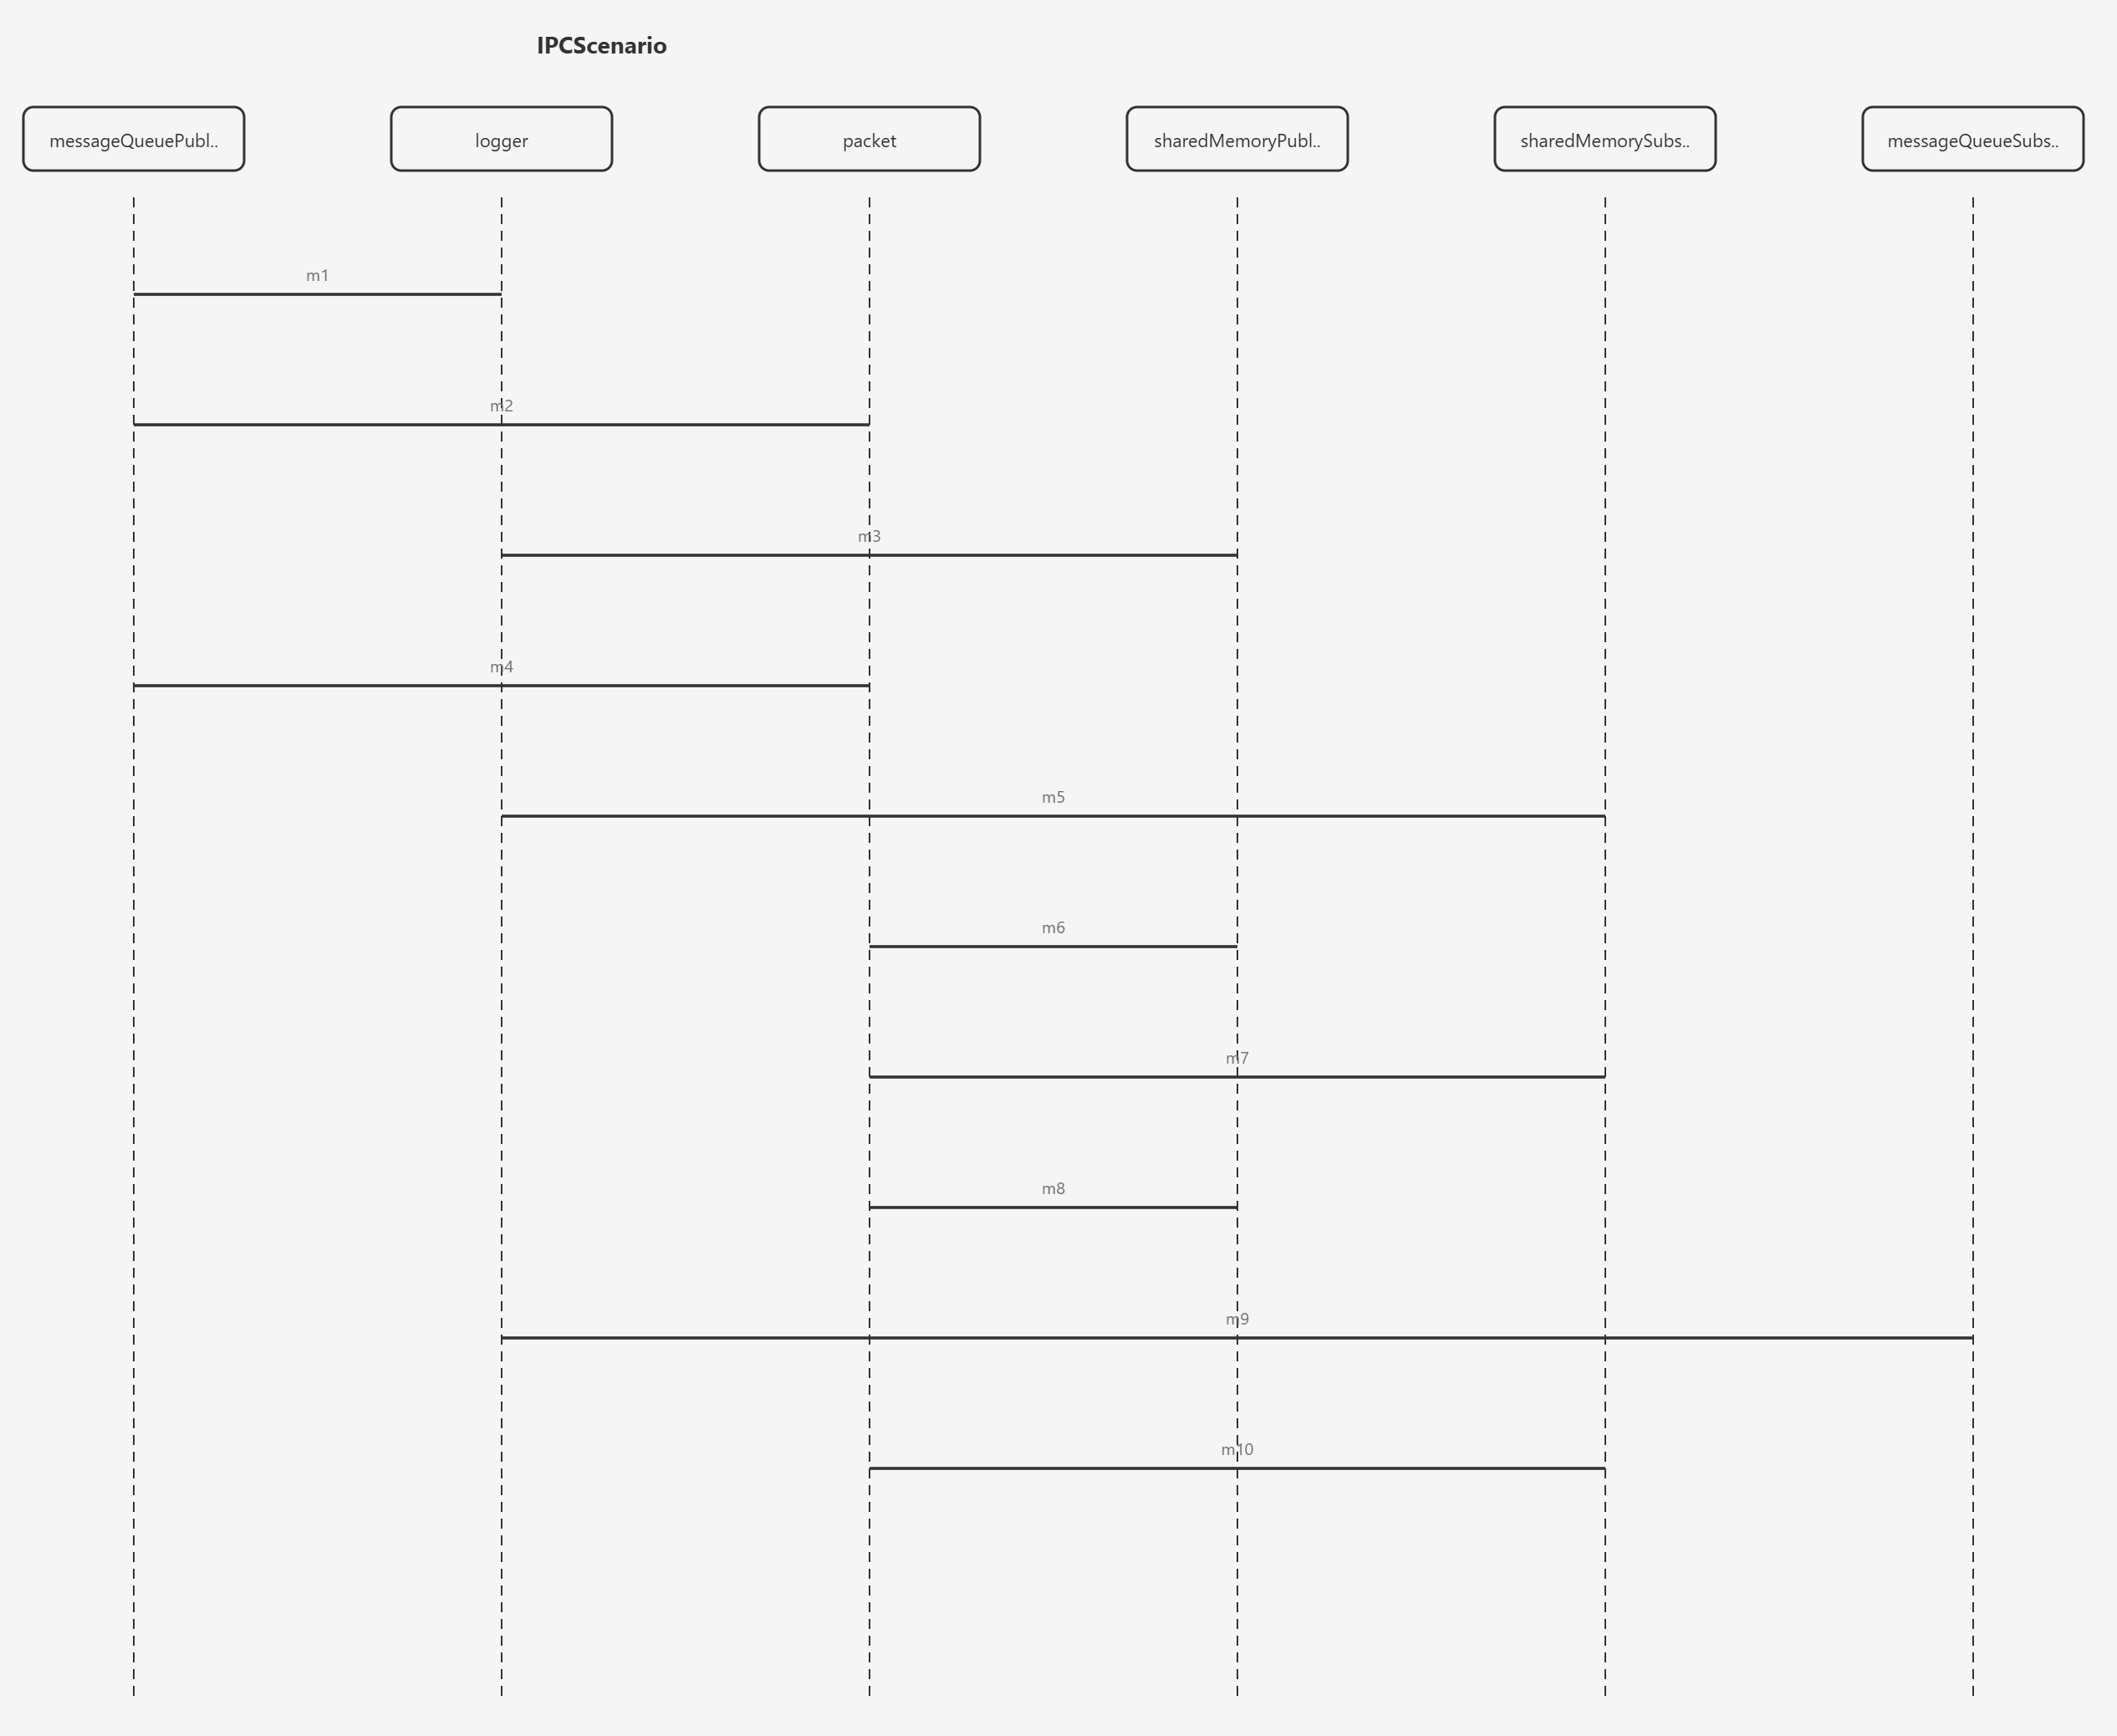
\includegraphics[width=\linewidth]{figures/sysmlv2 diagrams/ipcFlow.png}
    \caption{IPC scenario: message queue and shared memory publisher/subscriber
      interactions (MessageQueuePublisher, Logger, Packet, SharedMemoryPublisher,
      SharedMemorySubscriber, MessageQueueSubscriber).}
    \label{fig:sysml-ipc}
  \end{subfigure}
  \caption{SysML v2 sequence diagrams: IDC (left) and IPC (right).}
\end{figure}

\begin{figure}[htbp]
  \centering
  \begin{subfigure}[t]{0.48\textwidth}
    \centering
    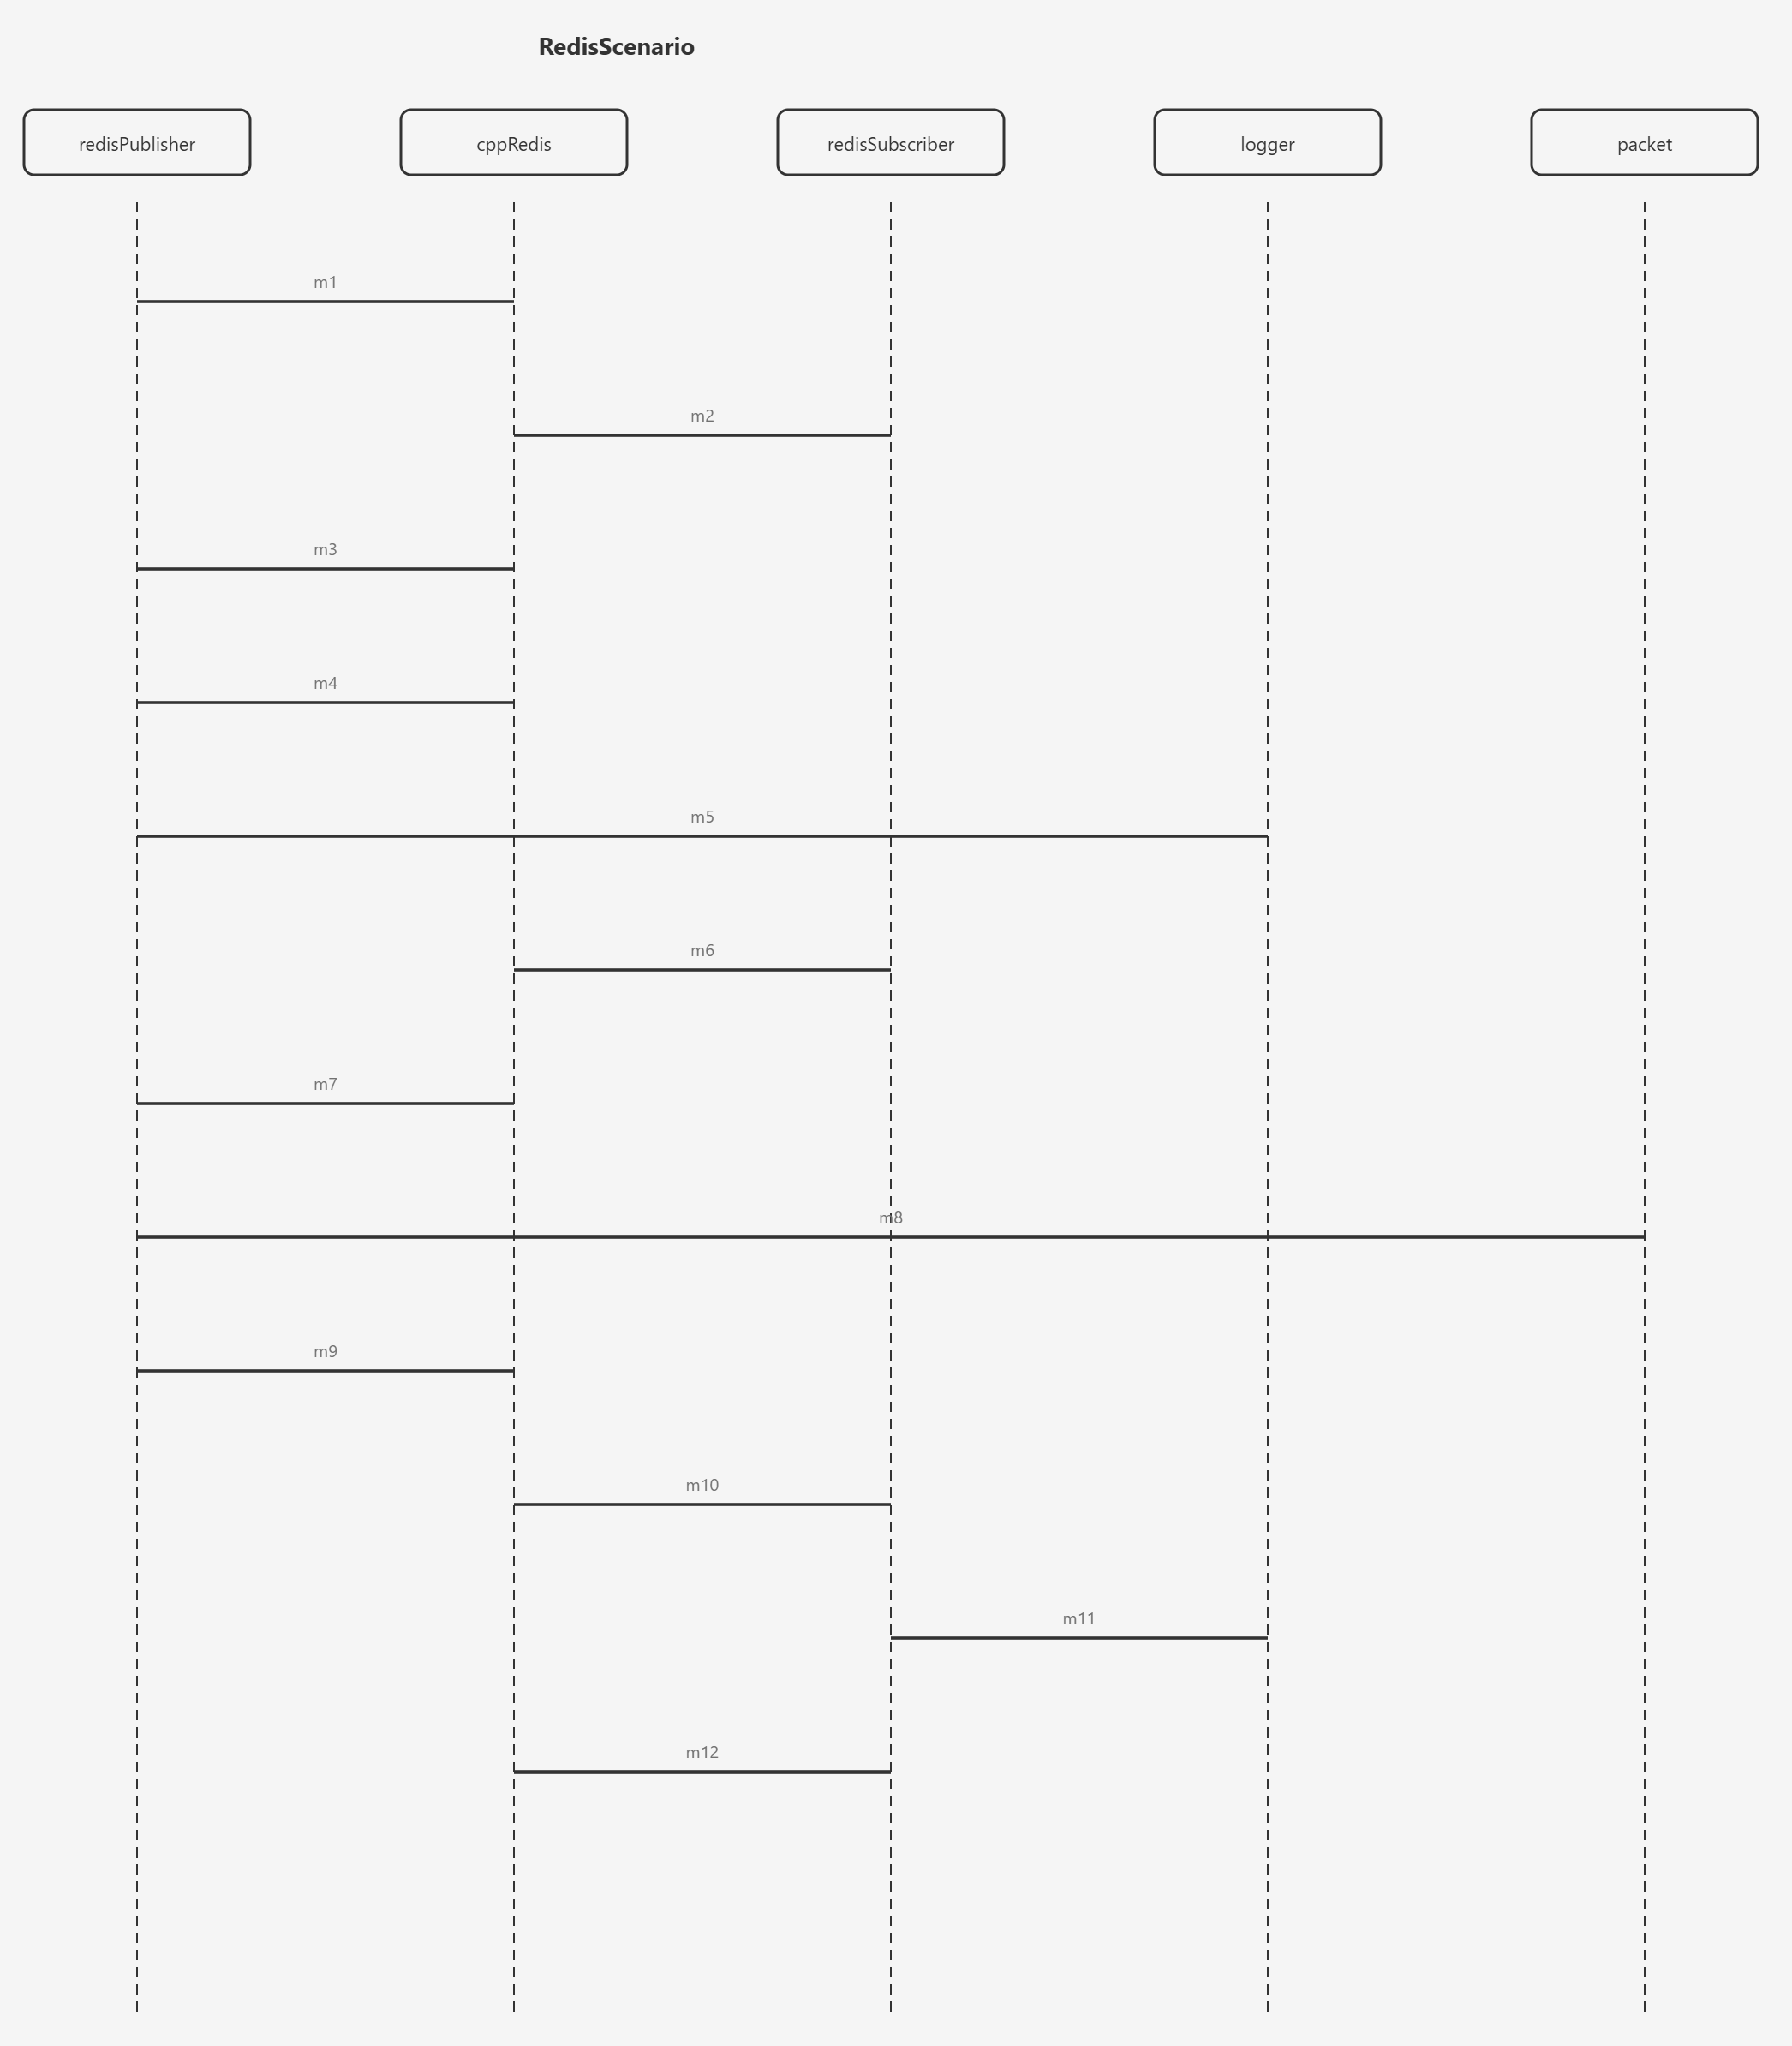
\includegraphics[width=\linewidth]{figures/sysmlv2 diagrams/redisFlow.png}
    \caption{Redis scenario: Redis-based publish-subscribe communication path
      (RedisPublisher, CppRedis, RedisSubscriber, Logger, Packet).}
    \label{fig:sysml-redis}
  \end{subfigure}
  \hfill
  \begin{subfigure}[t]{0.48\textwidth}
    \centering
    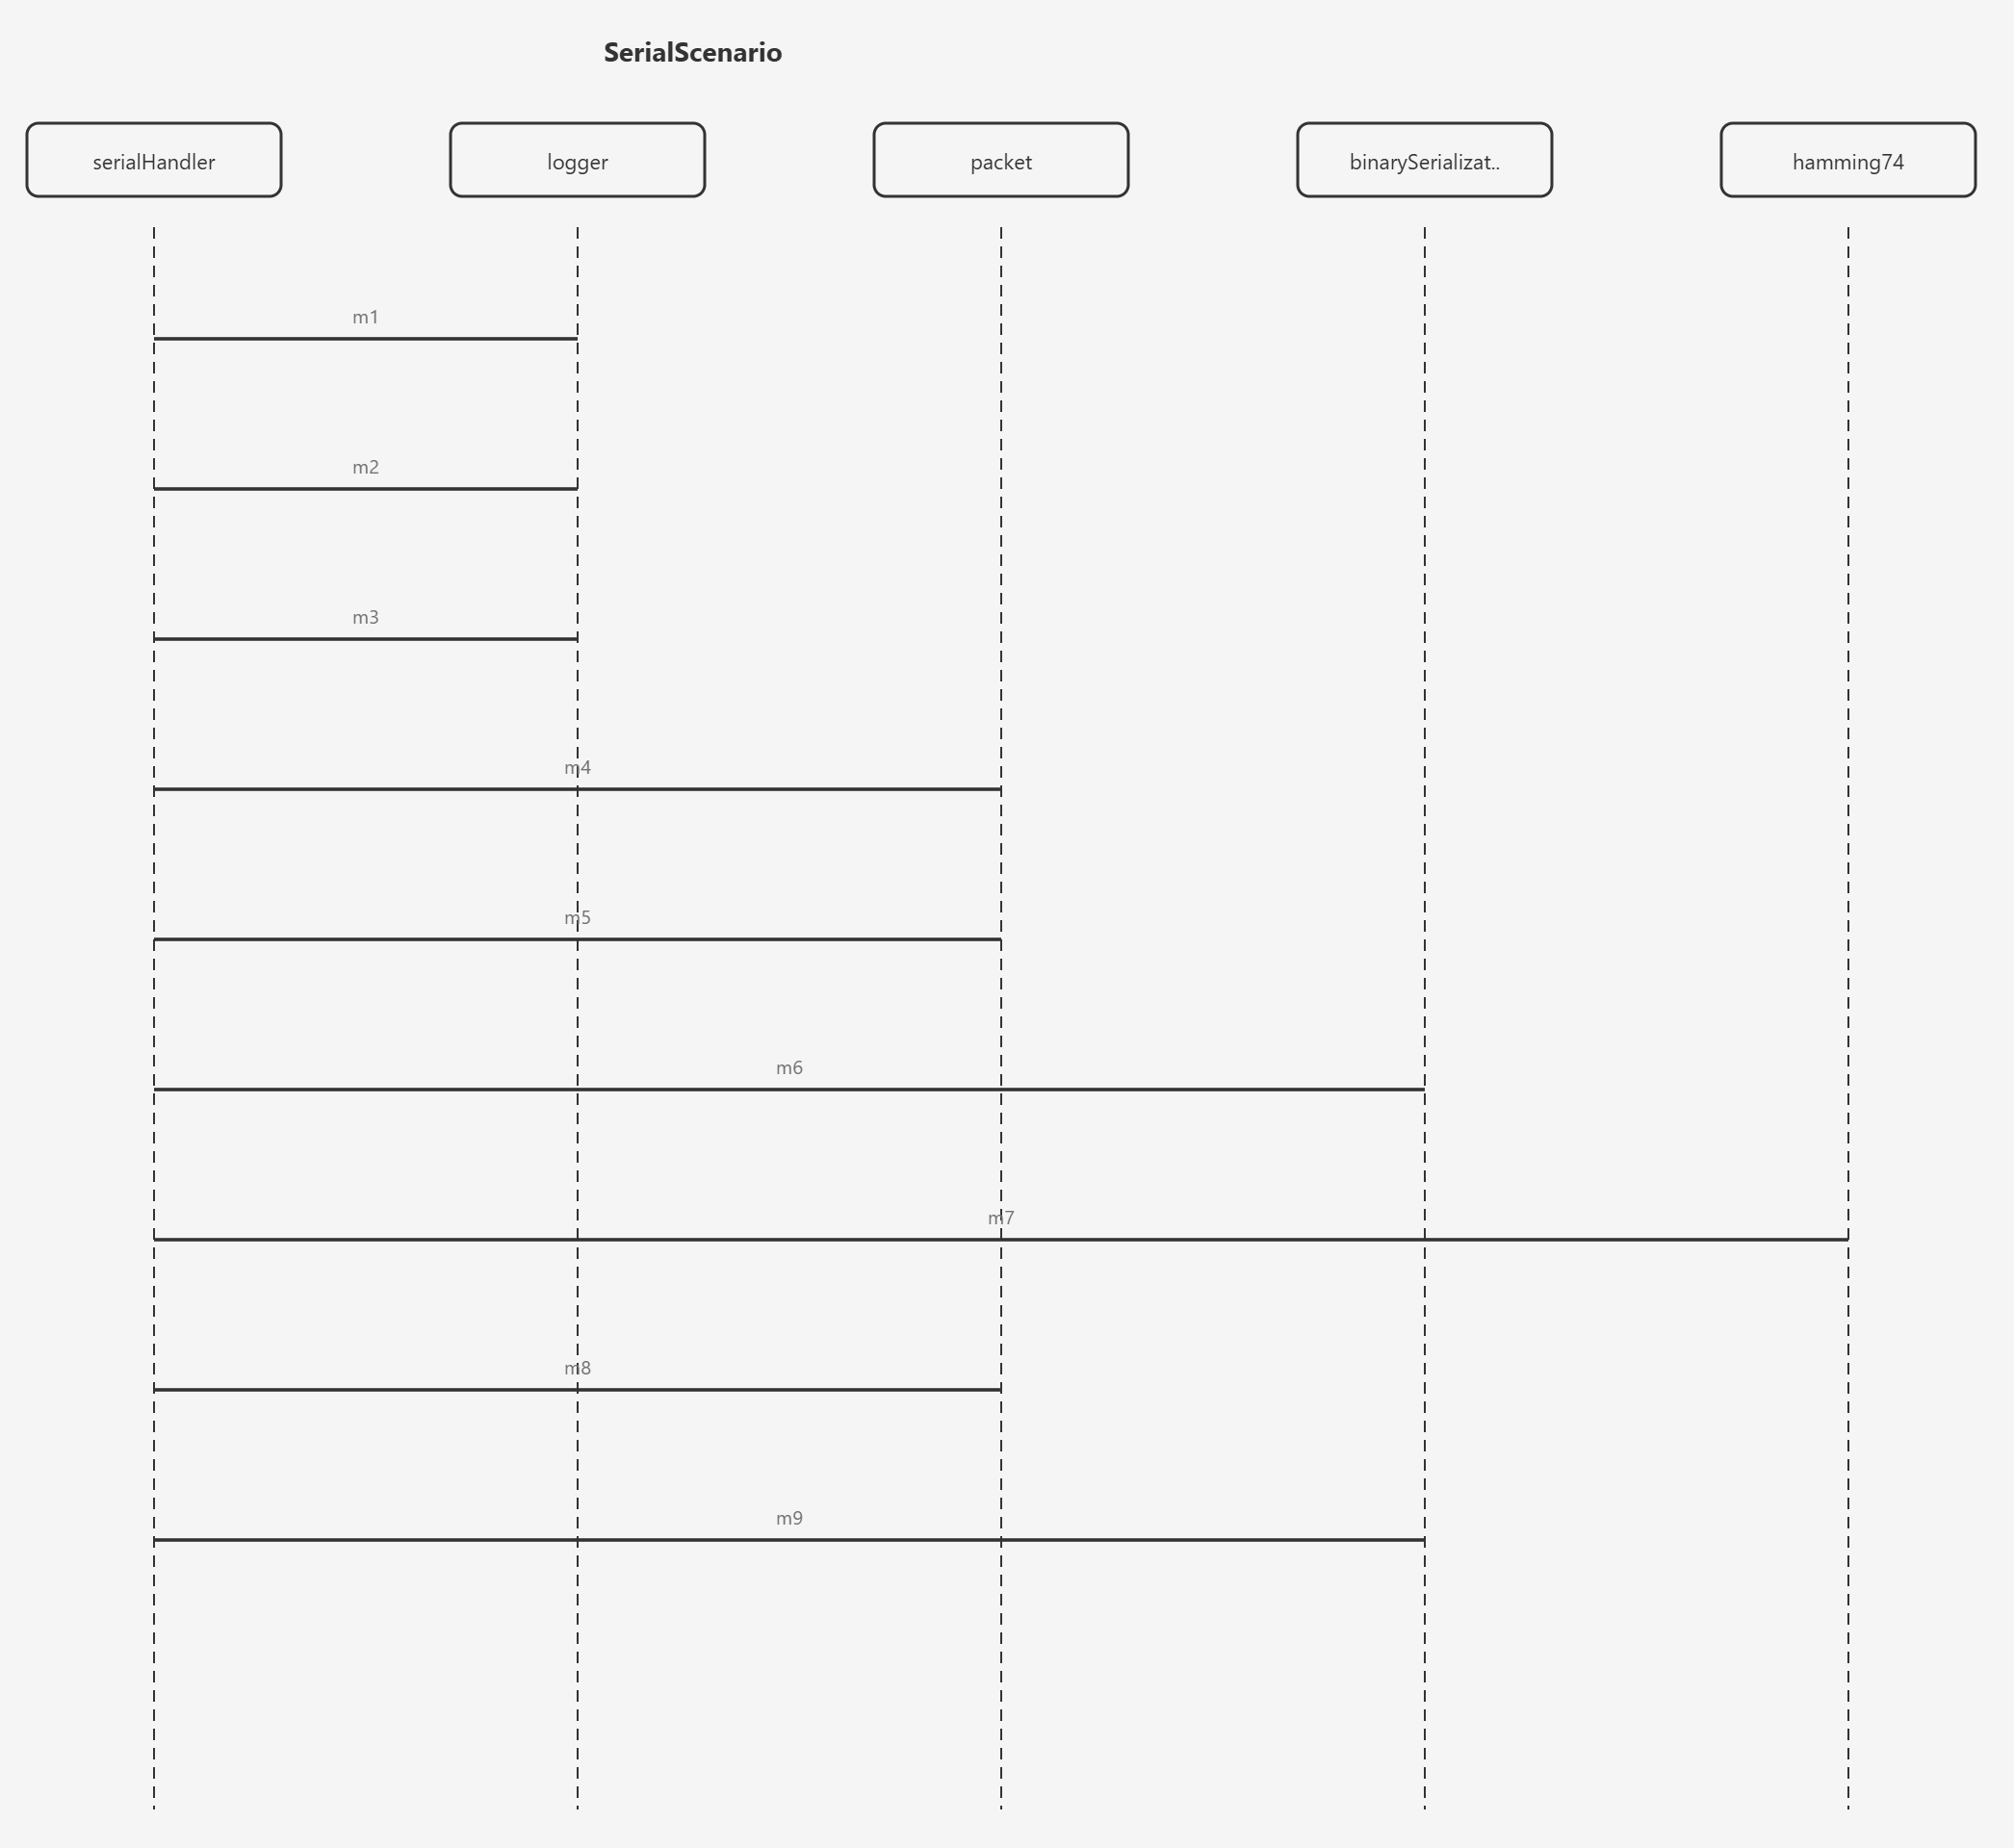
\includegraphics[width=\linewidth]{figures/sysmlv2 diagrams/serialFlow.png}
    \caption{Serial scenario: data serialisation interactions (SerialHandler,
      Logger, Packet, BinarySerialization, Hamming74).}
    \label{fig:sysml-serial}
  \end{subfigure}
  \caption{SysML v2 sequence diagrams: Redis (left) and Serial (right).}
\end{figure}

\begin{figure}[H]
  \centering
  \begin{subfigure}[t]{0.48\textwidth}
    \centering
    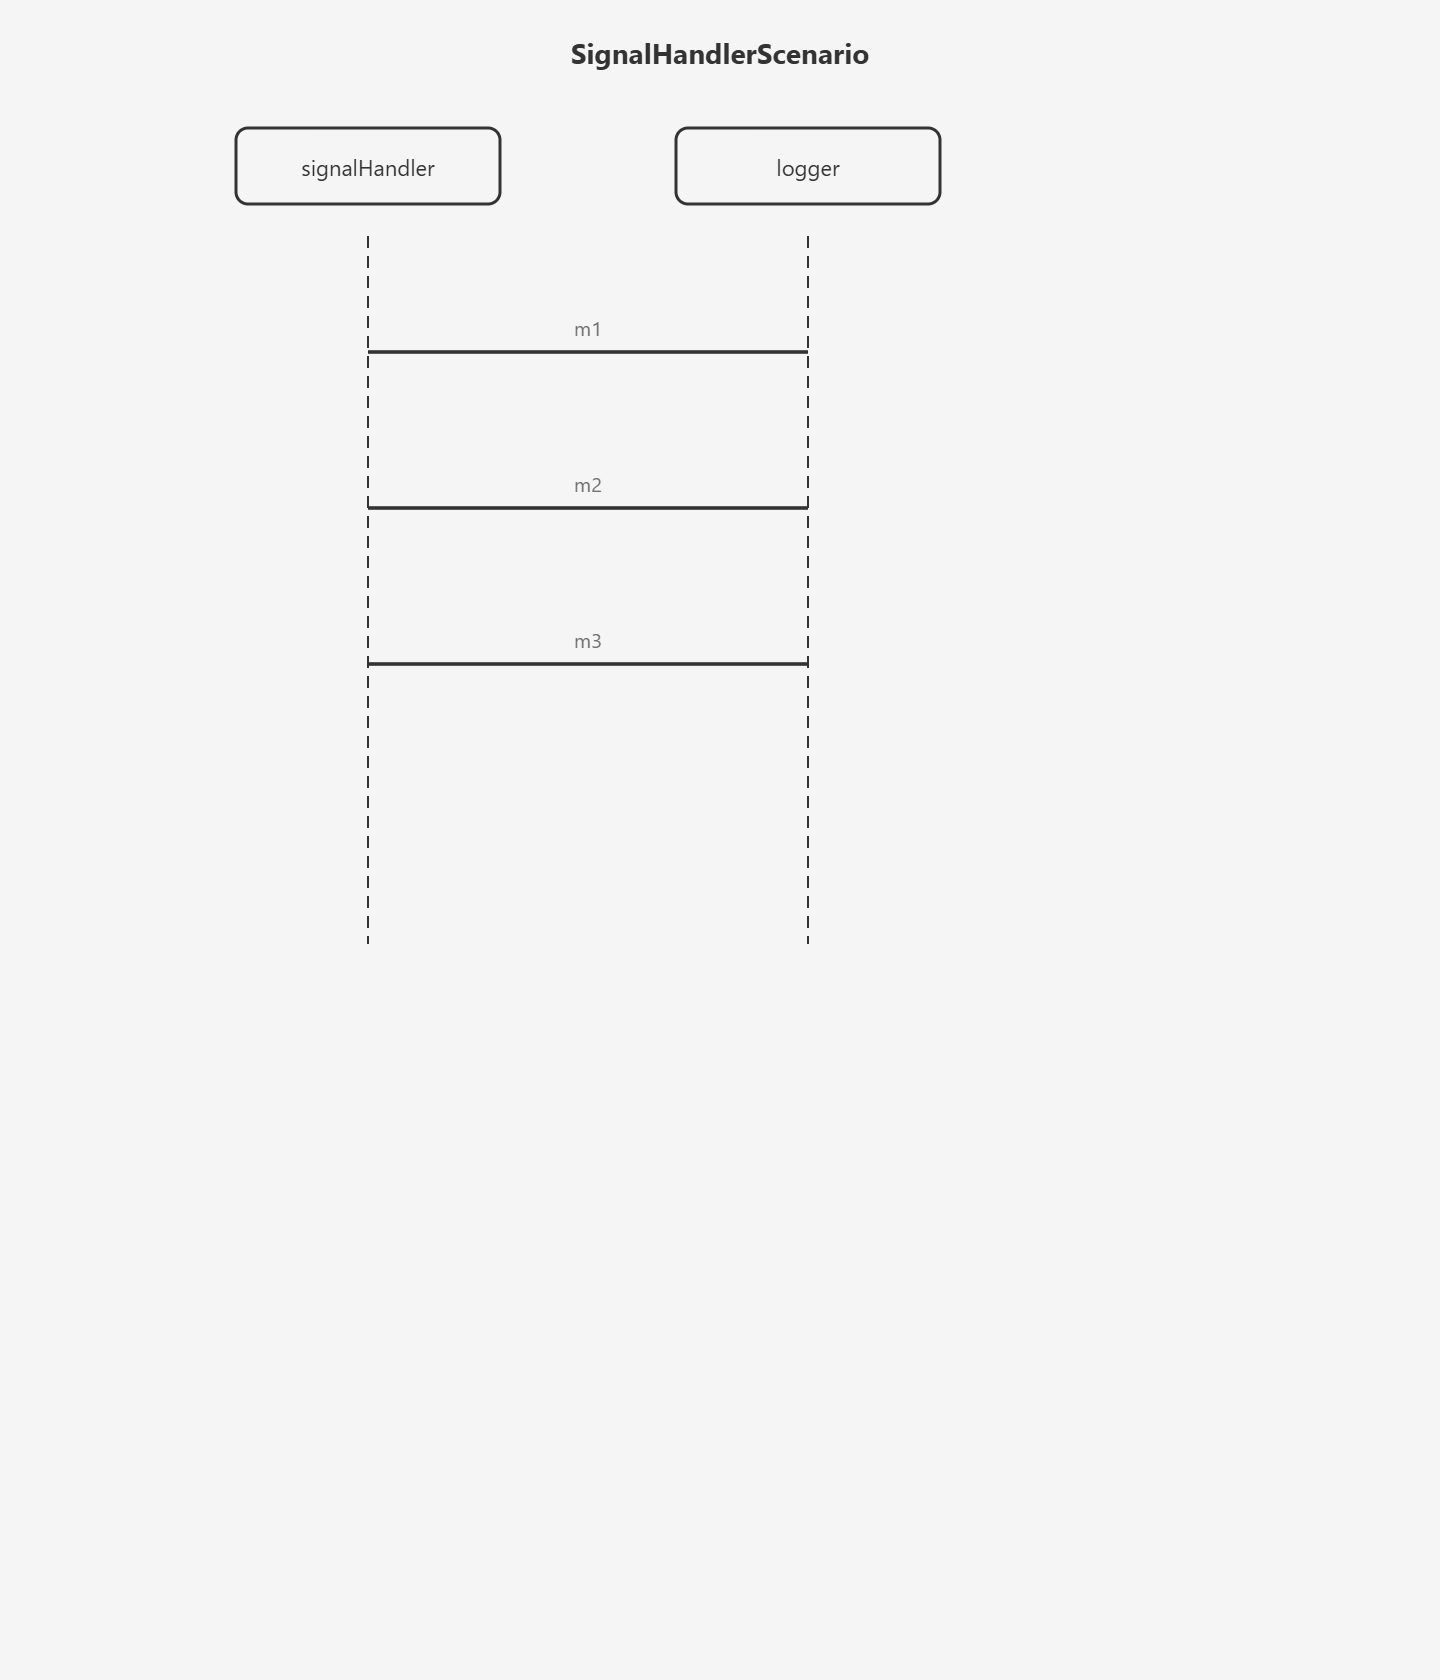
\includegraphics[width=\linewidth]{figures/sysmlv2 diagrams/signalHandlerFlow.png}
    \caption{Signal handler scenario: signal handling to logging interaction
      path (SignalHandler, Logger).}
    \label{fig:sysml-signalhandler}
  \end{subfigure}
  \hfill
  \begin{subfigure}[t]{0.48\textwidth}
    \centering
    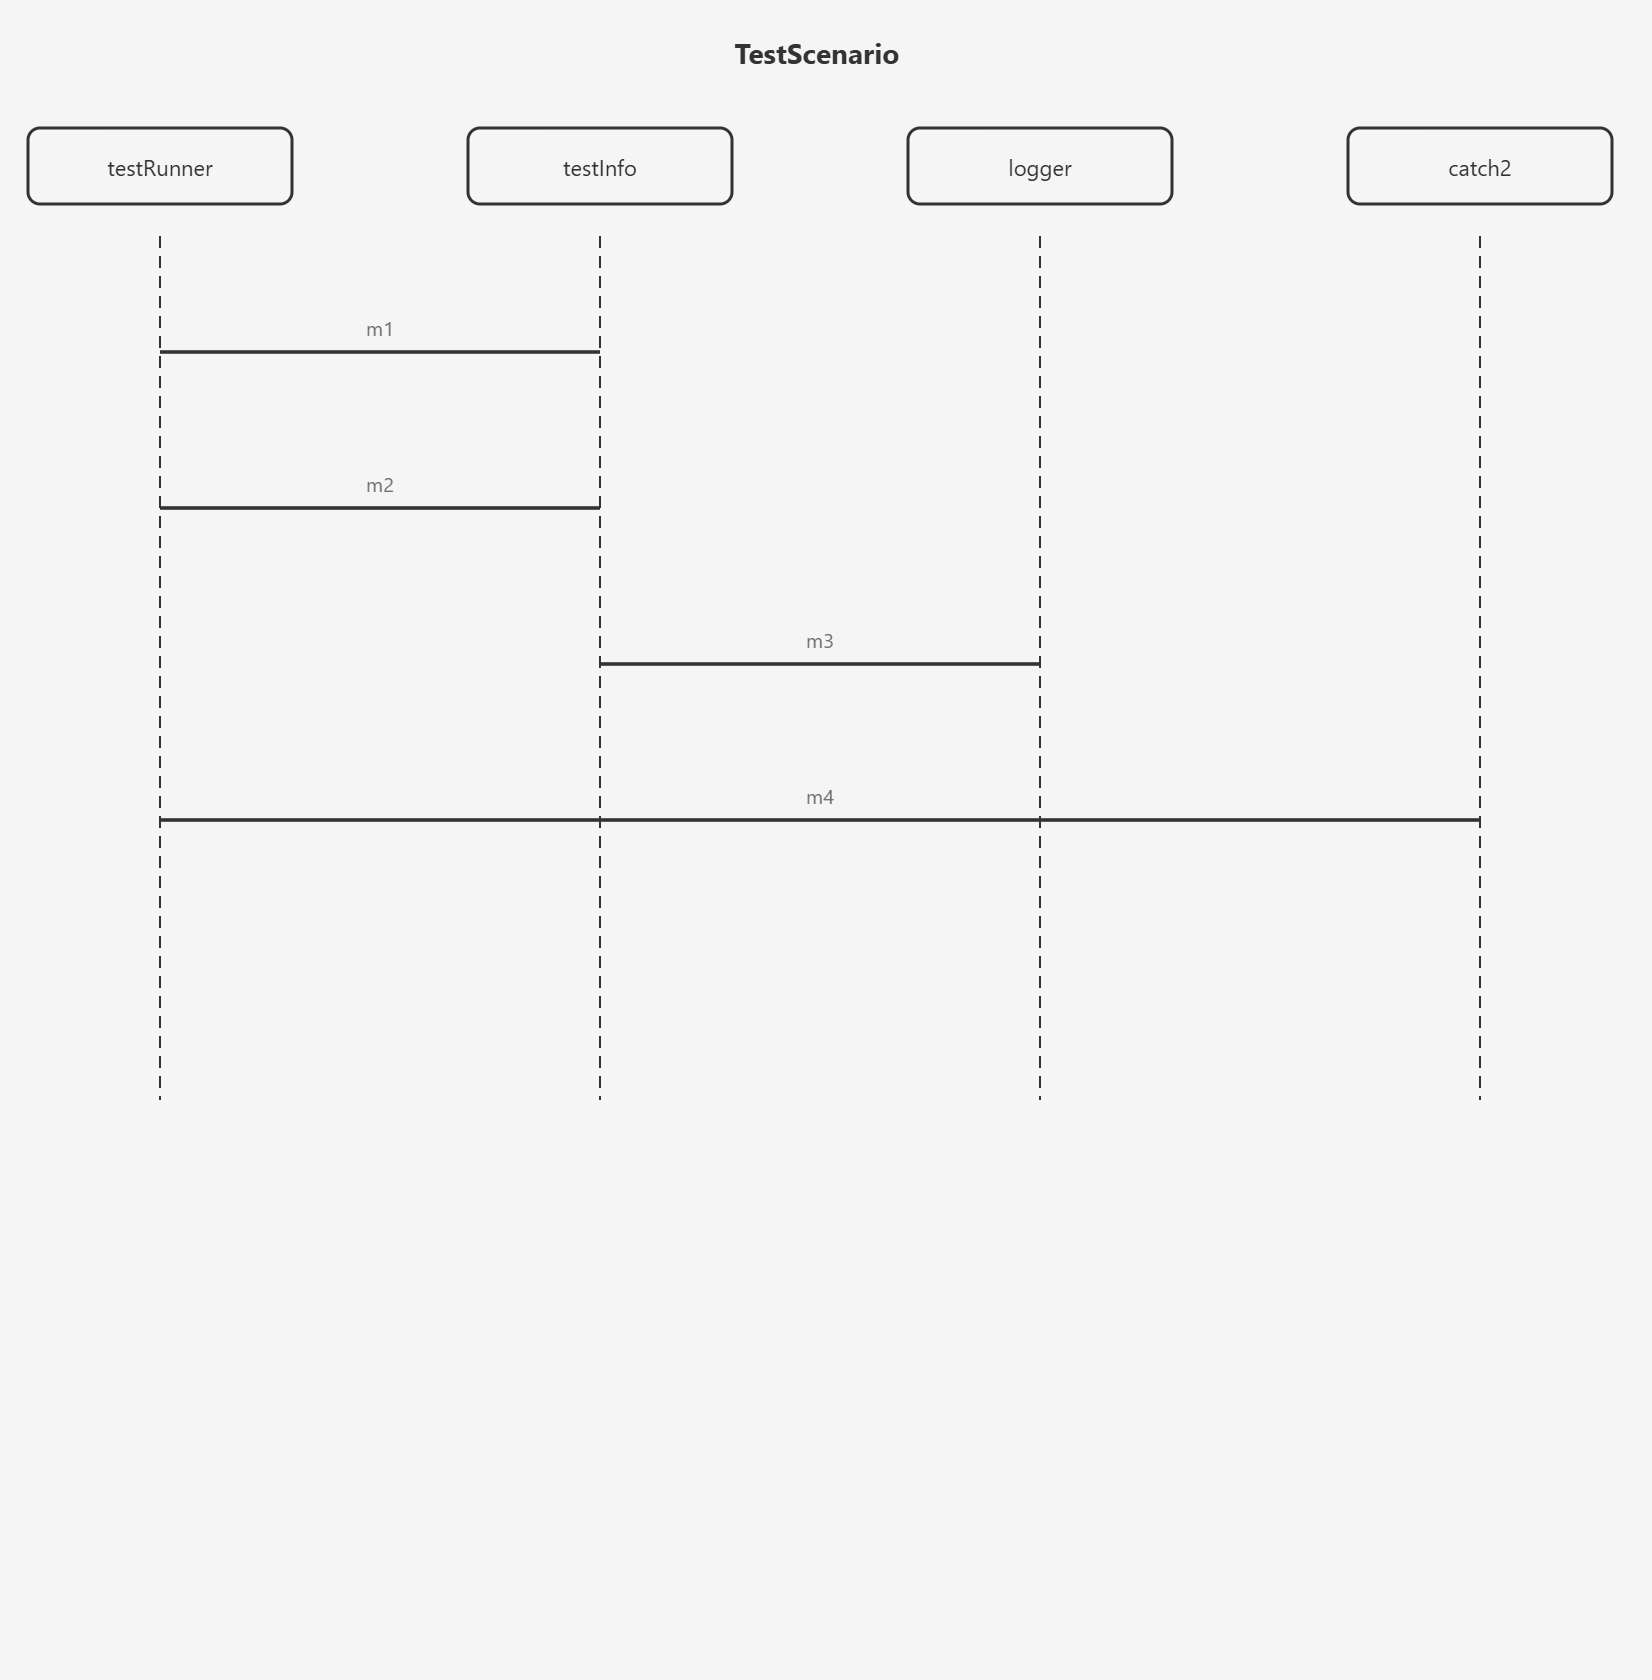
\includegraphics[width=\linewidth]{figures/sysmlv2 diagrams/testFlow.png}
    \caption{Test scenario: test runner and test info interactions
      (TestRunner, TestInfo, Logger, Catch2).}
    \label{fig:sysml-test}
  \end{subfigure}
  \caption{SysML v2 sequence diagrams: Signal handler (left) and Test (right).}
\end{figure}

\begin{figure}[htbp]
  \centering
  \begin{subfigure}[t]{0.48\textwidth}
    \centering
    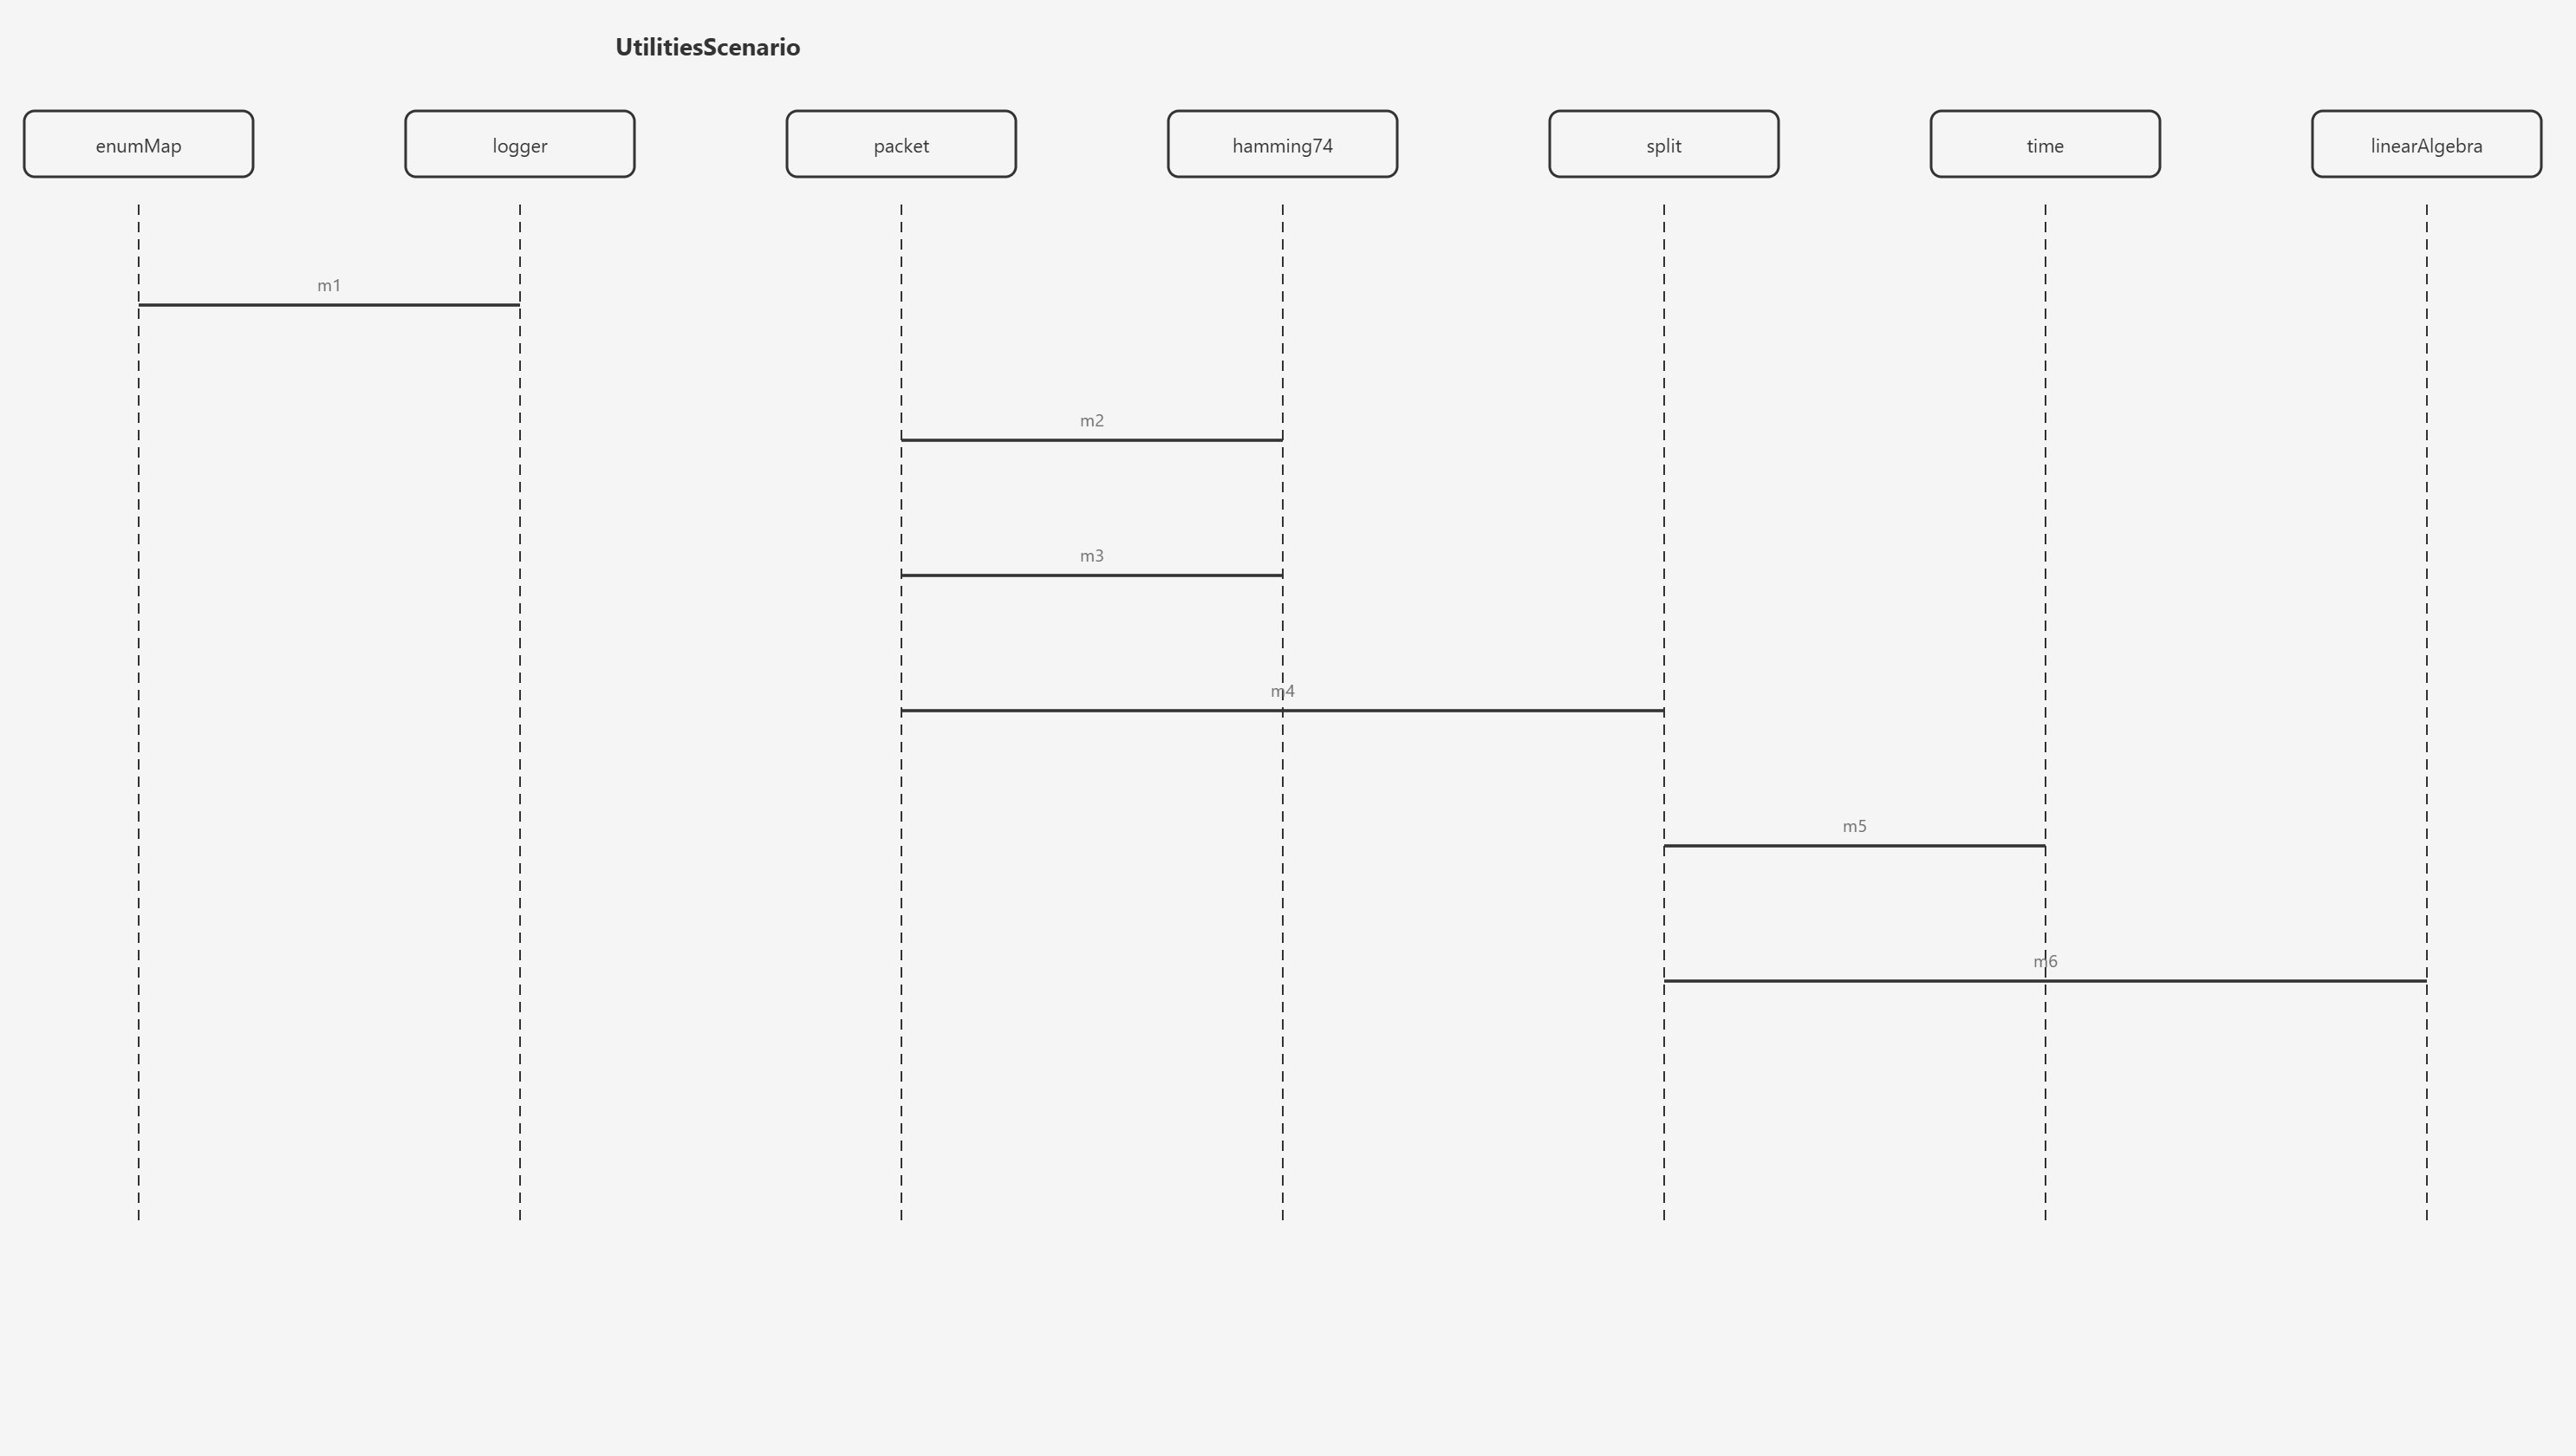
\includegraphics[width=\linewidth]{figures/sysmlv2 diagrams/utilitiesFlow.png}
    \caption{Utilities scenario: cross-utility interactions (EnumMap, Logger,
      Packet, Hamming74, Split, Time, LinearAlgebra).}
    \label{fig:sysml-utilities}
  \end{subfigure}
  \hfill
  \begin{subfigure}[t]{0.48\textwidth}
    \centering
    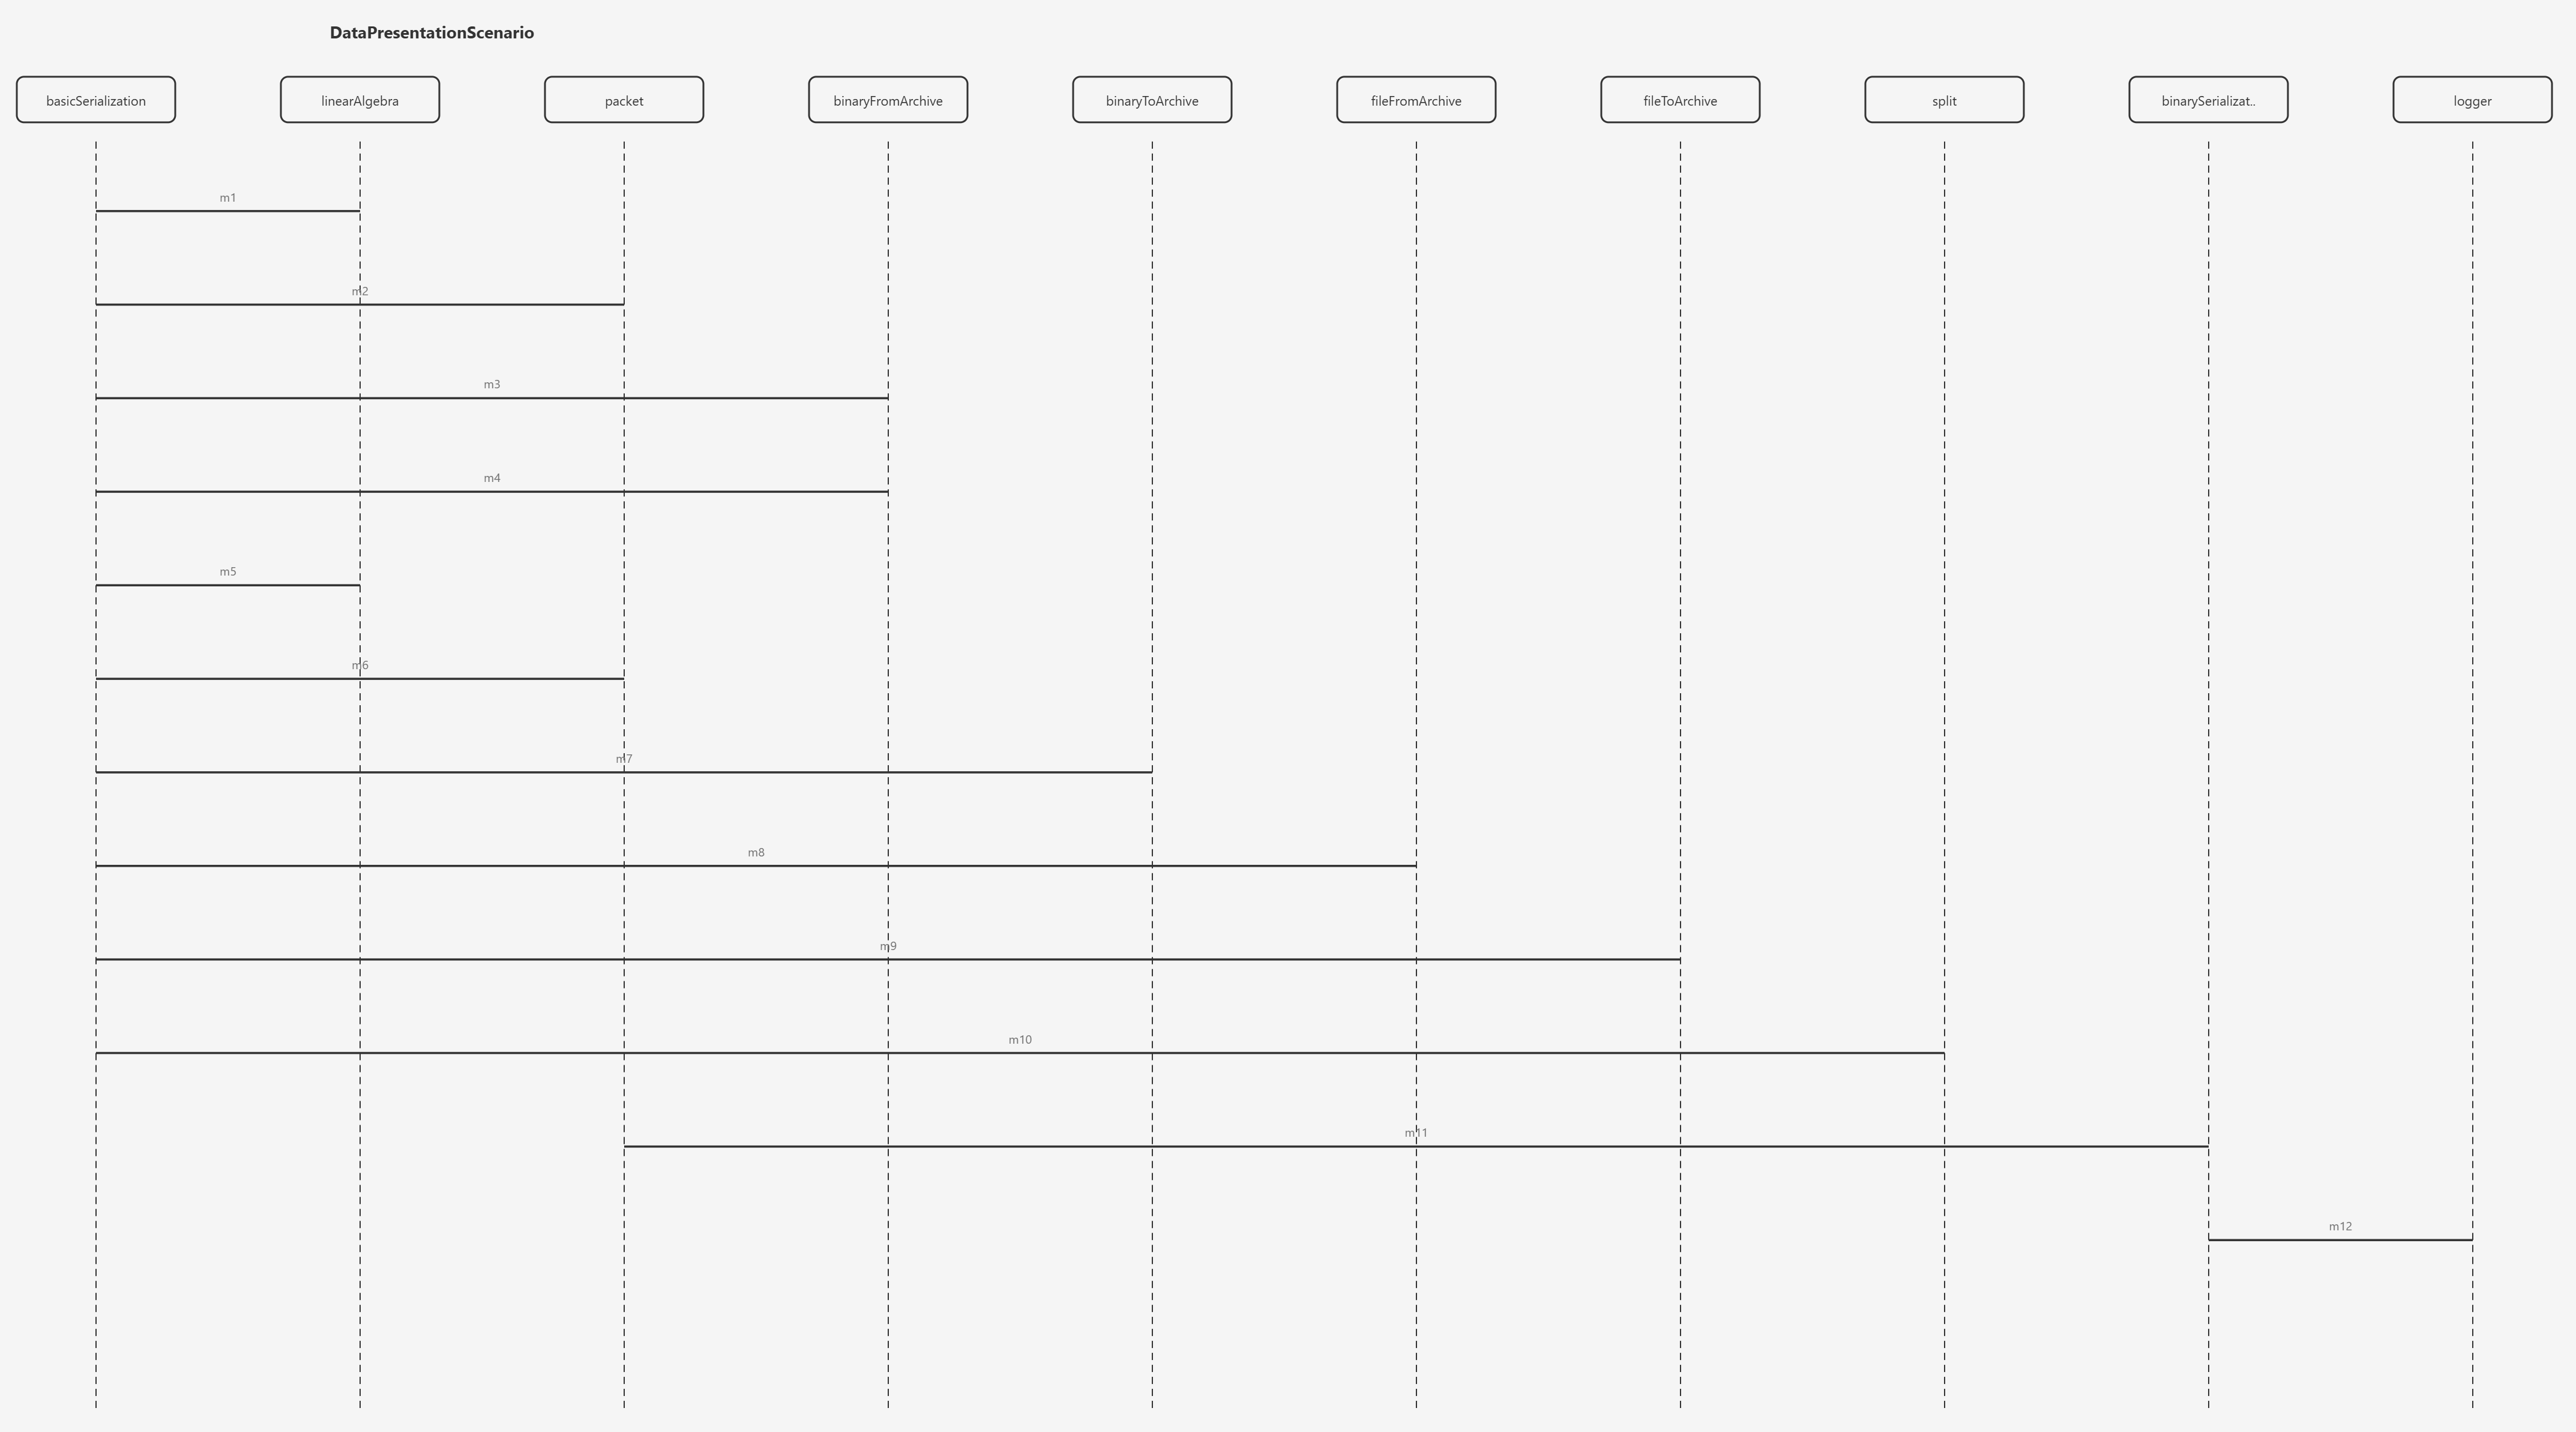
\includegraphics[width=\linewidth]{figures/sysmlv2 diagrams/dataPresentationFlow.png}
    \caption{Data presentation scenario: Hamming74 encoding/decoding and
      packet-level interactions.}
    \label{fig:sysml-datapresentation}
  \end{subfigure}
  \caption{SysML v2 sequence diagrams: Utilities (left) and Data presentation (right).}
\end{figure}

\begin{figure}[H]
  \centering
  \begin{subfigure}[t]{0.48\textwidth}
    \centering
    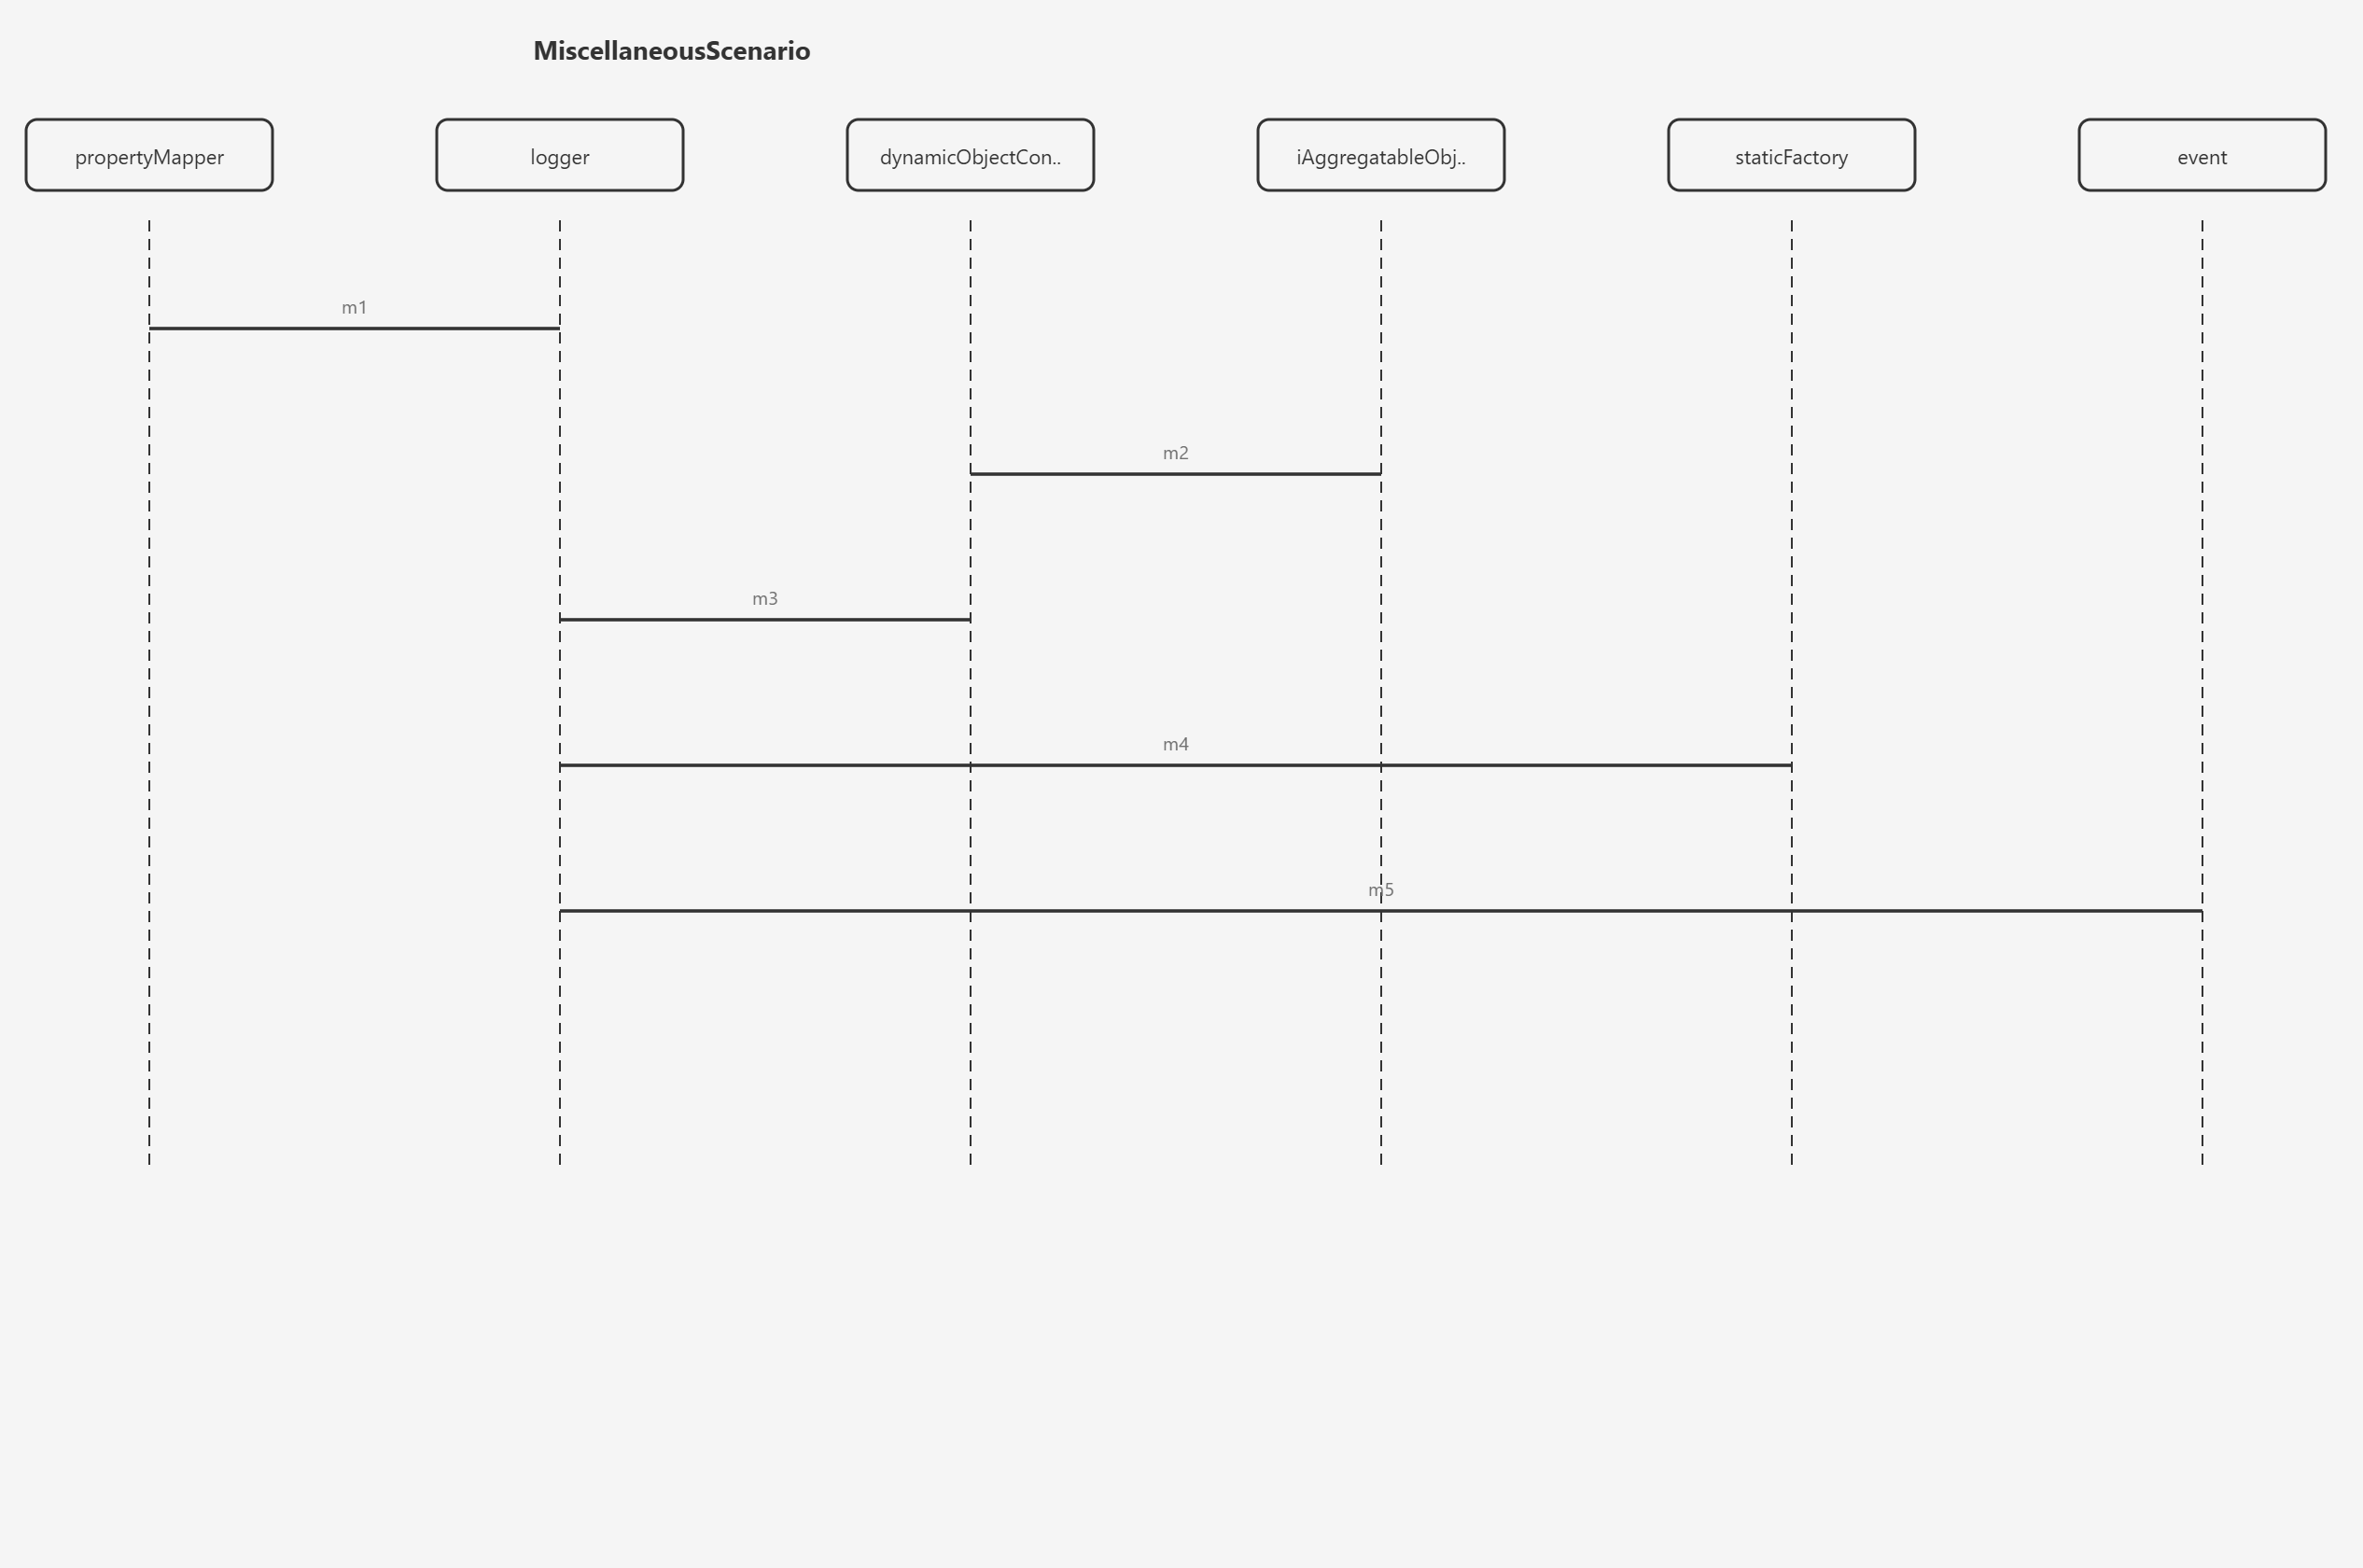
\includegraphics[width=\linewidth]{figures/sysmlv2 diagrams/miscellaneousFlow.png}
    \caption{Miscellaneous scenario: PropertyMapper, Logger,
      DynamicObjectContainer, IAggregatableObject, StaticFactory, and Event
      interactions.}
    \label{fig:sysml-misc}
  \end{subfigure}
  \hfill
  \begin{subfigure}[t]{0.48\textwidth}
    \centering
    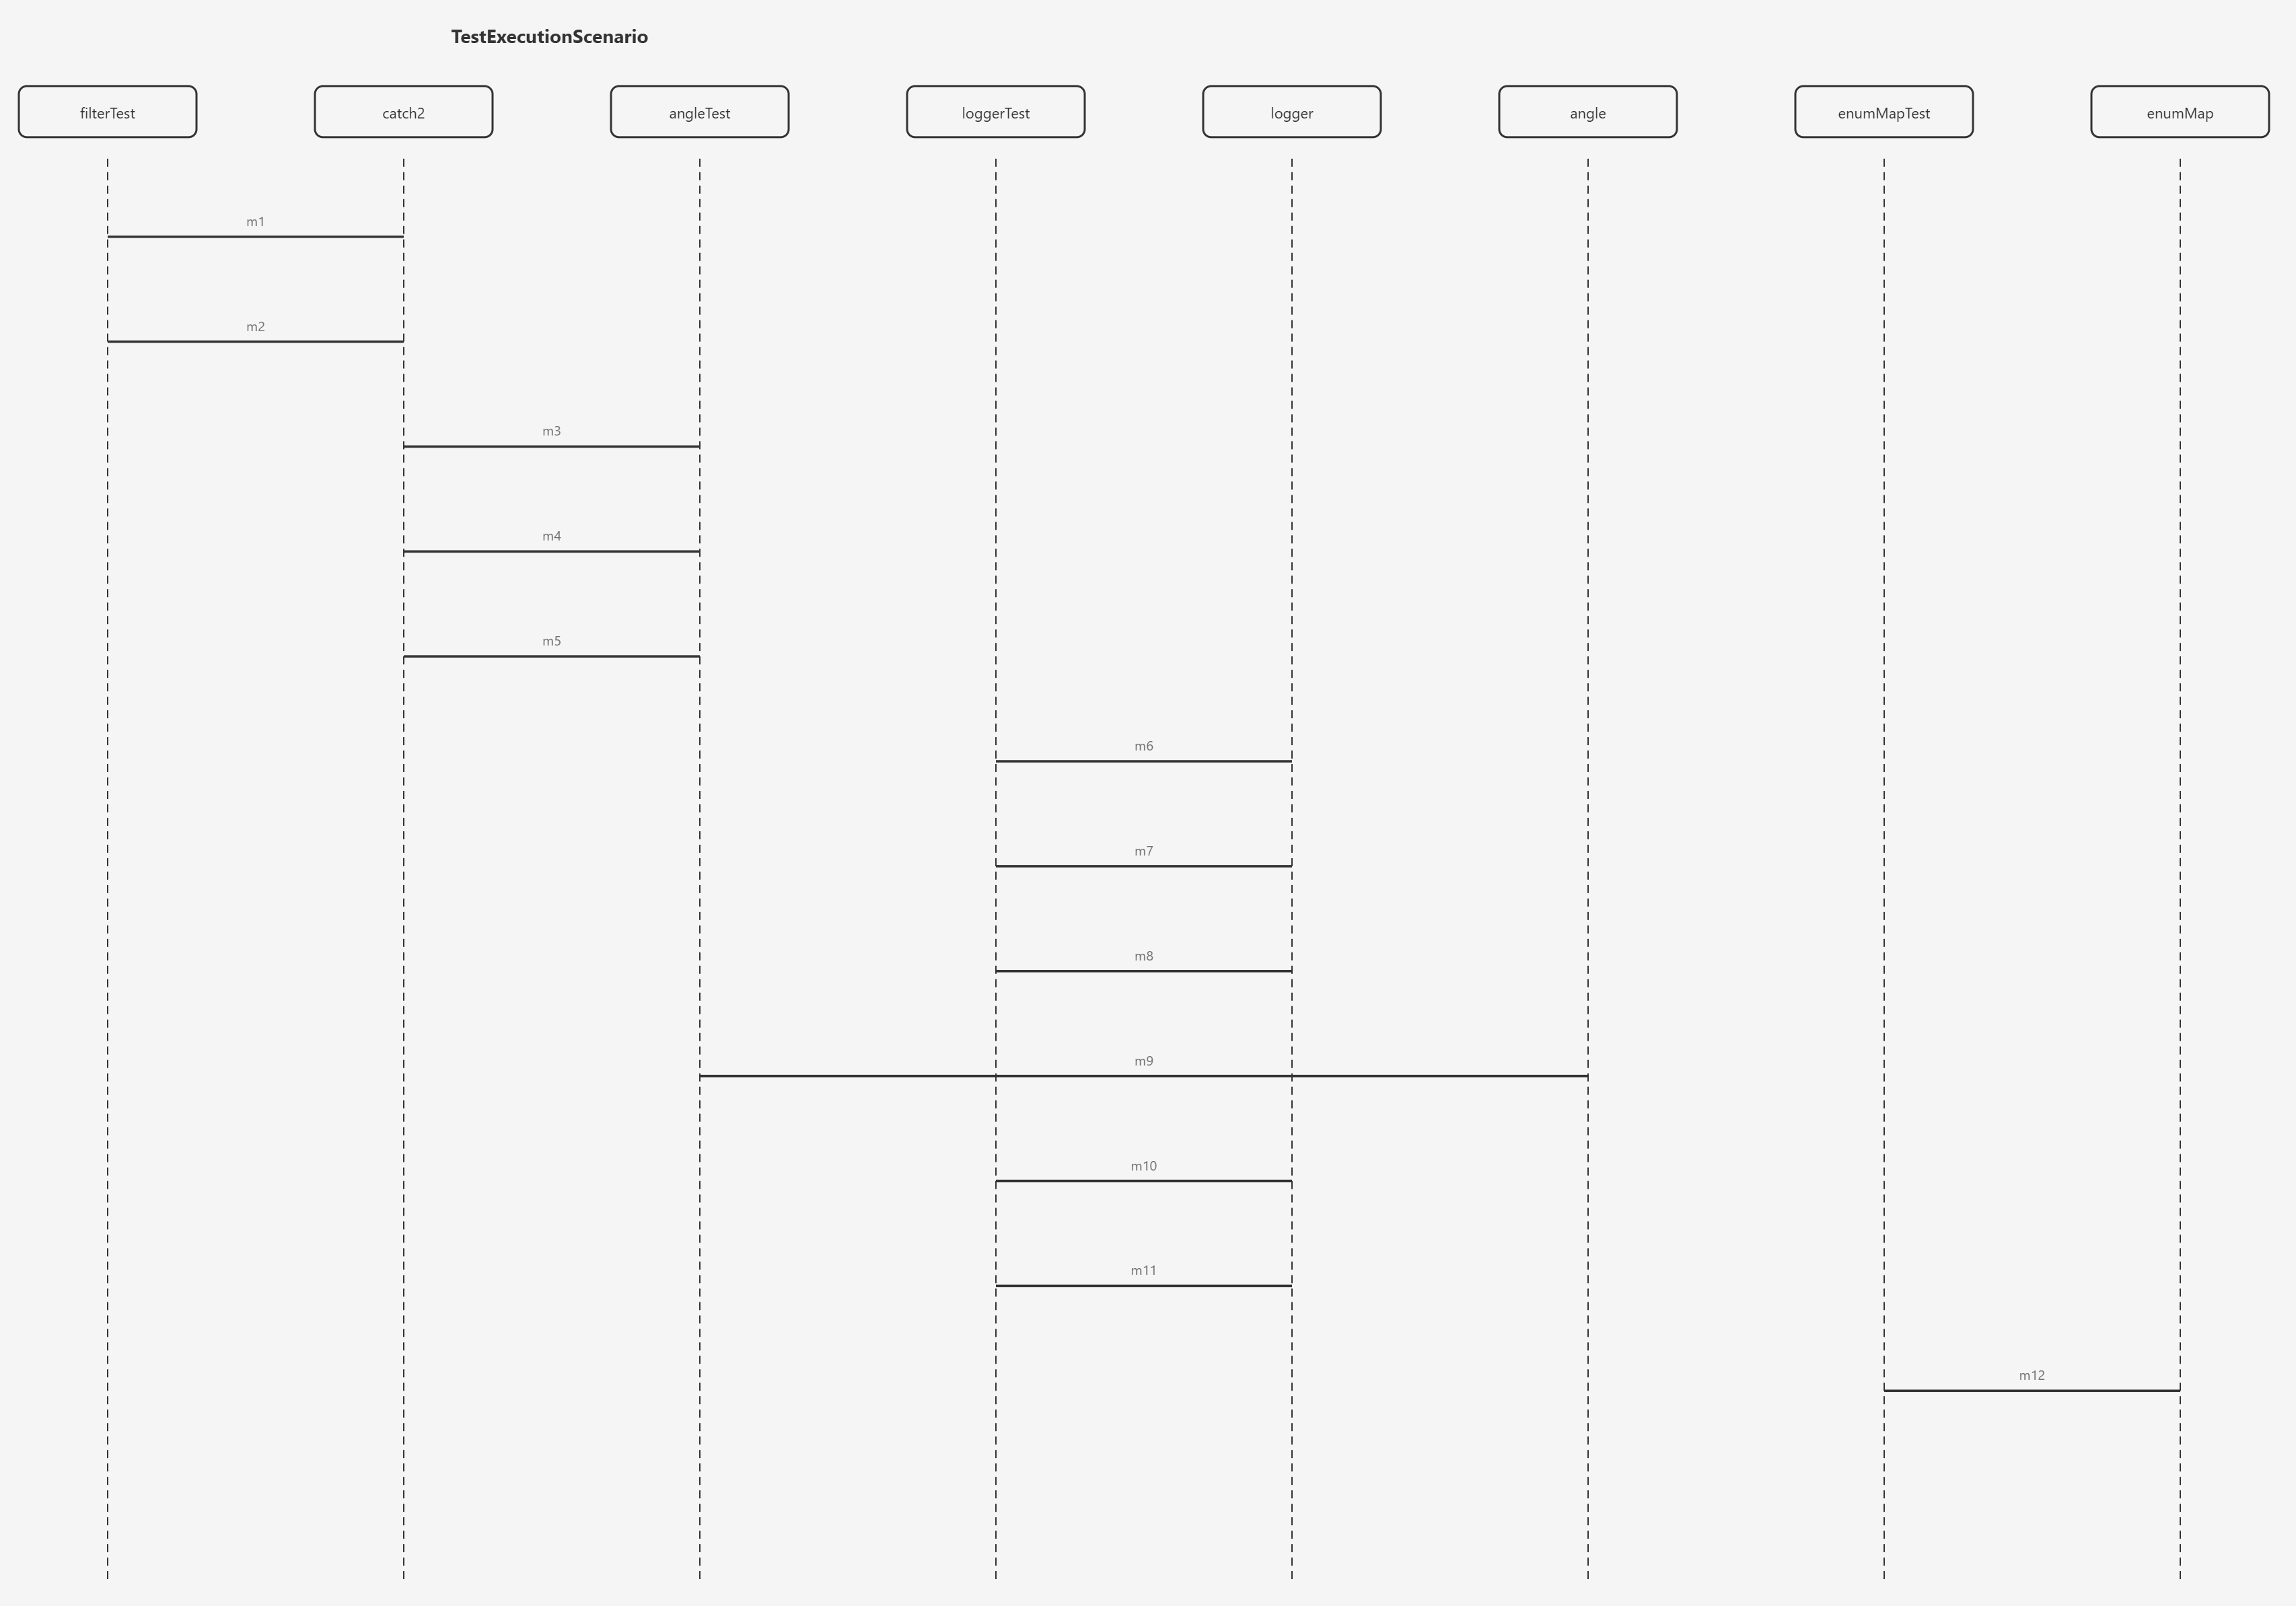
\includegraphics[width=\linewidth]{figures/sysmlv2 diagrams/testExecutionFlow.png}
    \caption{Test execution scenario: test framework interactions (FilterTest,
      Catch2, AngleTest, LoggerTest, Logger, Angle, EnumMapTest, EnumMap).}
    \label{fig:sysml-testexecution}
  \end{subfigure}
  \caption{SysML v2 sequence diagrams: Miscellaneous (left) and Test execution (right).}
\end{figure}
